\documentclass[10pt]{article}

%%%%%%%%%%%%%%%%%%%%%%%%%%%%%%%%%%%%%%%%%%%%%
% Package Inclusion and Document Formatting %
%%%%%%%%%%%%%%%%%%%%%%%%%%%%%%%%%%%%%%%%%%%%%
\usepackage
{geometry,amsmath,amsthm,mathrsfs,amssymb,graphicx,bm,hyperref,url,pdfsync,
fancyhdr}
\pagestyle{fancy}
\numberwithin{equation}{section}
%%%%%%%%%%%%%%%%%%%
% Custom Commands %
%%%%%%%%%%%%%%%%%%%
\newcommand{\n}{\noindent}
\newcommand{\norm}[1]{\left\lvert#1\right\rvert}
\newcommand{\avg}[1]{\left\langle#1\right\rangle}
\newcommand{\figref}[1]{Figure \ref{#1}}
%%%%%%%%%%%%%%%%%%%%%%%%%%
% Title Page Information %
%%%%%%%%%%%%%%%%%%%%%%%%%%

\title{Notes for PHYS 232: Stellar Structure}
\author{Bill Wolf}
\date{\today}

\begin{document}

\vfill\maketitle\vfill \newpage

\tableofcontents \newpage

%%%%%%%%%%%%%%%%%%%%%%
% January 9, 2012 %
%%%%%%%%%%%%%%%%%%%%%%

\section{Introduction}
	\emph{Monday, January 9, 2012}
	\subsection{The HR Diagram} 
	Most stars shine predominantly in the optical range of the 
electromagnetic spectrum. As a result, we get most of our information about 
stars by observing their optical output.  It makes sense, then, that we 
might organize stars by there color, which is indicative of their surface 
temperature. When plotting a population of stars' luminosities against 
their surface temperature, we note a strong correlation between the two. As 
it turns out, the controlling parameter for these quantities is the mass of 
the star, at least while the star is on the \textbf{Main Sequence} (stars 
burning hydrogen to helium). The correlation between the mass of a main-
sequence star and its luminosity is incredibly strong (see HR diagram 
examples).
	\begin{figure}
		\centering
		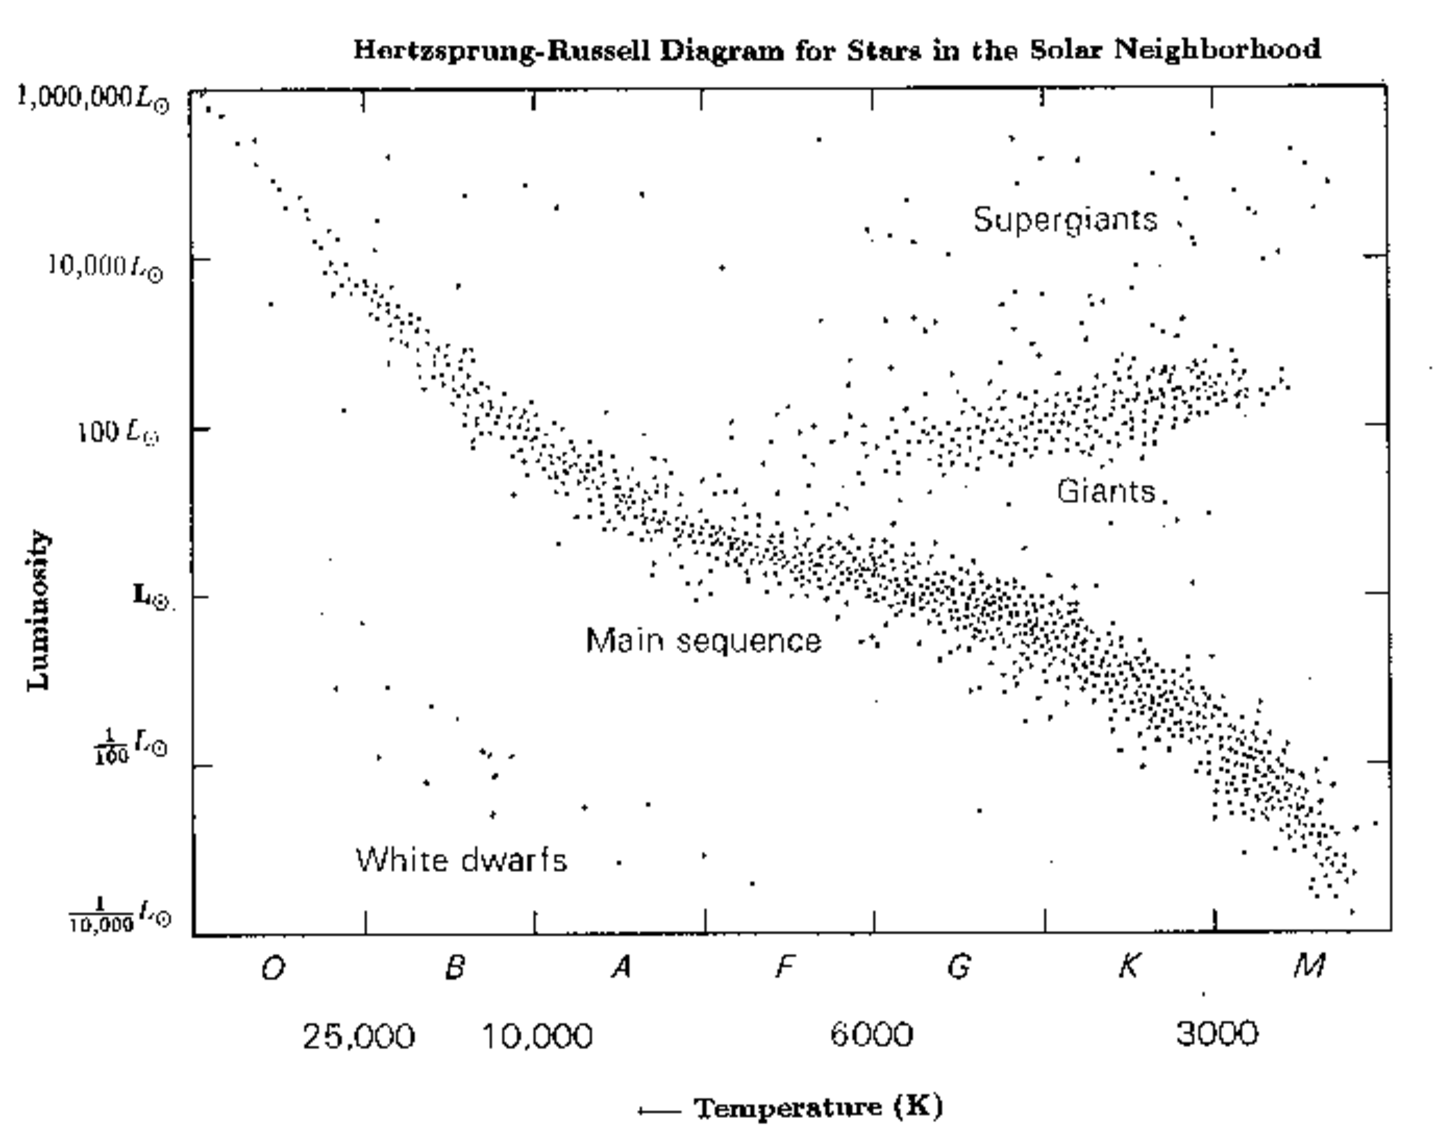
\includegraphics[width=6in]{hr_local.pdf}
		\caption{An HR diagram for stars in the local neighborhood 
(shamelessly stolen from Google Images)}
		\label{HR.1f}
	\end{figure}
	\subsection{Conditions for a Star on the HR Diagram}
	We are interested in knowing what defines the regime where a star can 
reside in a particular $L,\,T_{\mathrm{eff}}=[L/(4\pi\sigma_{\mathrm{SB}}
R^2)]^{1/4}$. Why, for example, is there a dynamical range in the 
luminosity spanning over six orders of magnitude, while only a range of a 
factor of about 5 in the effective temperature? To gain some perspective, 
we might observe the number of stars as a function of brightness. We 
organize these stars by their \textbf{spectral type} (a rough measure of 
how big the star is) and find their approximate \textbf{mass density} (the 
amount of mass contained in these stars per unit volume):
	\begin{center} 
	\begin{tabular}{l l}
		Spectral Type & $\rho\ (M_\odot/\mathrm{pc^3})$\\
		\hline
		O-B & 0.4\\
		A-F & 4\\
		G-M & 40\\
		WD's & 20
	\end{tabular}
	\end{center}
	Here we've used the standard labels for different spectral types, O, B, 
A, F, G, K, M, L, T, which are roughly in decreasing order of size and 
temperature (the reasoning for this scale is historical rather than 
logical, and the ordering is often remembered by the mnemonic, ``Oh Be A 
Fine Gal/Guy, Kiss Me! Less Talk!''). We see that the big, bright stars 
form an exceedingly small portion of the amount of stellar mass in our 
galaxy. We will find that this is because large stars exhaust their fuel 
much more quickly than smaller stars, and thus live and die much faster. 
We'll now observe another type of classification of stars used in our 
neighborhood, the Milky Way Galaxy.
		
	\subsubsection{Population I Stars}
	From Earth, the center of the galaxy is approximately 8.5 kpc away. 
Meanwhile, the disk is only about 100 pc wide.  We've observed that stars 
in the thin disk (commonly known as \textbf{Population I Stars}) are 
orbiting at the orbital velocity with only a small amount of axial and 
radial motion. They are essentially dynamically cold and in nearly circular 
orbits. This is indeed where most of the \textbf{interstellar medium} (ISM) 
resides, causing much of the star formation in the galaxy. This region is 
also very metal rich. That is, compared to other parts of the universe, 
there is a much higher concentration of elements heavier than helium 
present. We will denote the mass fraction of these ``metals'' with the 
letter $Z$, and in this region, we have $Z\sim 1-2\,\%$. These metals come 
from a previous generation of stars, who died in the past, giving off the 
metals we now have.	
	
	\subsubsection{Population II Stars}
	 \textbf{Population II Stars} reside mostly in the spheroid in the 
center of the galaxy. These are older stars in regions where star formation 
is largely shut down. Typically they are metal poor, with metallicities as 
low as $Z=10^{-4}Z_\odot$. Kinematically, they are often on radial orbits 
(rather than their more azimuthal population I counterparts in the disk). 
We typically say that the globular clusters are part of this population. 
Sometimes these stars are seen passing through the disk at velocities 
comparable to the orbital velocities, and are easily identified due to 
their high velocities and unique spectra (due to the low metallicities).

%%%%%

\section{A Simple Hydrostatic Atmosphere}
	 \subsection{Scale Height and Column Depth}
	 Before tackling the physics of stars, we first consider a simple toy 
model-- the isothermal, plane parallel atmosphere. This model is somewhat 
applicable to the thin stellar atmosphere near the surface of a star, where 
curvature can be neglected and the acceleration due to gravity is nearly 
uniform.\\
	 
	 \n Consider an atmosphere where the local acceleration due to gravity, 
$\mathbf{g}$ is constant in value and direction. The atmosphere is composed 
of an isothermal ideal gas with temperature $T$. We wish to find the 
distribution of particles in this atmosphere.\\
	 
	 \n In a strictly statistical sense, we would expect the energy 
distribution to be comparable to $e^{-E/kT}$ (recall that the atmosphere is 
isothermal, so the average kinetic energy is uniform throughout). In our 
case, the energy of particles is linear in height, so we expect this 
probability to be proportional to $e^{-mgh/kT}$.\\
	 
	 \n We will let $m_B\approx m_p$ be the baryon mass, $\mu$ be the mean 
molecular mass (measured in AMU), and $\rho$ is the density in $\mathrm{g
\,cm^{-3}}$. We suppose that the gas is in hydrostatic balance, so we have
	 \begin{equation}
	 	\label{ippa.1} \frac{dP}{dz}=-\rho g
	 \end{equation}
	 Combining this with the ideal gas law,
	 \begin{equation}
	 	\label{ippa.2} P=nkT
	 \end{equation}
	We find that
	\begin{equation}
		\label{ippa.3} kT\frac{dn}{dz}=-m_p\mu ng
	\end{equation}
	which in turn gives us
	\begin{equation}
		\label{ippa.4} \frac{d\ln n}{dz}=-\frac{m_p\mu g}{kT}
	\end{equation}
	Solving this differential equation gives the expected result
	\begin{equation}
		\label{ippa.5} n(z)=n(0)\exp\left(-\frac{m_p\mu gz}{kT}\right)=n
(0)\exp\left(-\frac{z}{h}\right)
	\end{equation}
	where we have defined the \textbf{scale height} $h\equiv kT/(\mu m_pg)
$, which is the e-folding distance in number density. As it turns out, the 
scale height for earth's atmosphere is approximately 10 km. This model is 
really only valid in cases where $h\ll R$, (where $R$ is the size of the 
object), so we now investigate the ratio of these two quantities:
	\begin{equation}
		\label{ippa.6} \frac{h}{R}=\frac{kT}{\mu m_p\frac{GM}{R^2}R}=\frac
{1}{\mu}\frac{kT/m_p}{GM/R}\sim \frac{v_{\mathrm{th}}^2}{v_{\mathrm{esc}}
^2}\ll 1
	\end{equation}
	So if this approximation is valid, the thermal velocities of particles 
are typically much smaller than the escape velocity of the central body, so 
a star could retain its own atmosphere (thankfully, Earth does the same to 
its atmosphere!) For stars, we will find that $kT_c/m_p\sim GM/R$. Then, 
\eqref{ippa.6} tells us that
	\begin{equation}
		\label{ippa.7} \frac{h}{R}\sim \frac{T_{\mathrm{eff}}}{T_c}.
	\end{equation}
	This tells us that stars are quite sharp-edged (their scale heights are 
very small compared to their radii). We can also deduce a physical meaning 
for the scale height as being how far a particle needs to fall to gain an 
energy comparable to $kT$.\\
	
	\n From the ideal gas law, we can easily see that the pressure will 
also fall off exponentially in this isothermal atmosphere. However, let's 
explore the pressure a bit more. First, we return to the ideal gas law,
	\begin{equation}
		\label{ippa.8} P=\frac{\rho}{\mu m_p}kT=nkT
	\end{equation}
	and the condition for hydrostatic equilibrium,
	\begin{equation}
		\label{ippa.9} dP=-\rho g\,dz.
	\end{equation}
	We now integrate \eqref{ippa.9} from $z=z$ to $z\to \infty$:
	\begin{align}
		\label{ippa.10} P(\infty)-P(z)&=-\int_z^\infty \rho(z') g\,dz'\\
		\label{ippa.11} P(z) &= g\int_z^\infty \rho(z')\,dz
	\end{align}
	Note that it is okay to take the integral to infinity so long as we are 
dealing with a constant $\mathbf{g}$. This result suggests the definition 
of the \textbf{column density}:
	\begin{equation}
		\label{ippa.12} y(z)\equiv \int_z^\infty \rho(z)\,dz
	\end{equation}
	On the surface of the earth, the column density is approximately 
$y=1000\,\mathrm{g\,cm^{-2}}$. Think of it as the amount of mass sitting 
above you per unit area at a given altitude. The column density is an 
important number (for us) to determine the details of heat transport. For 
now though, we can write the pressure in this isothermal atmosphere in a 
compact form: $P(z)=gy(z)$.
	\subsection{Mean Molecular Weights}
	We'll now make a useful definition for calculating pressures and other 
useful quantities. For an ideal gas, the total pressure of a mixed gas is 
simply
	\begin{equation}
		\label{mmw.1} P=\sum_{i=1}^N n_ikT
	\end{equation}
	where $n_i$ are just the number densities for each ion. The number 
density is computed via
	\begin{equation}
		\label{mmw.2} n_i=\frac{X_i\rho}{A_im_p}.
	\end{equation}
	where $X_i$ is the mass fraction of the $i^{\mathrm{th}}$ ion with mass 
number $A_i$ and $\rho$ is the overall mass density. Then the ion pressure 
is given by (assuming total ionization)
	\begin{equation}
		\label{mmw.3} P_{\mathrm{ion}}=kT\sum\frac{X_i\rho}{A_im_p}=\frac
{kT\rho}{m_p}\sum\frac{X_i}{A_i}=\frac{kT\rho}{\mu_{\mathrm{ion}}m_p}.
	\end{equation}
	Where we have defined the \textbf{mean molecular weight} of the ions to 
be
	\begin{equation}
		\label{mmw.3a} \mu_{\mathrm{ion}}=\left[\sum\frac{X_i}{A_i}\right]^
{-1}
	\end{equation}
	For the electrons, we have (assuming total ionization)
	\begin{equation}
		\label{mmw.4} P_e=n_ekT=kT\left(\sum Z_in_i\right)=\frac{kT\rho}
{m_p}\sum\frac{Z_iX_i}{A_i}.
	\end{equation}
	(here $Z_i$ is the atomic number, not the metallicity). Then the total 
pressure is just the sum of these two,
	\begin{equation}
		\label{mmw.5} P=P_{\mathrm{ion}}+P_e=\frac{\rho kT}{m_p}\left(\frac
{1}{\mu_e}+\frac{1}{\mu_i}\right)
	\end{equation}
	So we define the overall mean molecular weight via
	\begin{equation}
		\frac{1}{\mu}\equiv \frac{1}{\mu_e}+\frac{1}{\mu_i}
	\end{equation}
	One might think of this as the average weight of a particle that 
supplies pressure within a gas. Later, we'll see that this quantity, and 
its evolution, plays a large and critical role in the the nature of stellar 
evolution. Since fusion tends to decrease the pressure support, the star 
must continuously readjust its structure so as to hold itself up.\\
	
%%%%%%%%%%%%%%%%%%%%%%
%  January 11, 2012  %
%%%%%%%%%%%%%%%%%%%%%%
	\n \textit{Wednesday, January 11, 2012}
	\subsection{Electric Fields in Stars}
	Imagine a pure, ionized hydrogen atmosphere which is, on the large 
scale, electrically neutral. We wish to find the scale height in a plasma 
of ionized hydrogen. In this plasma, we have $n_p=n_e$ due to electric 
neutrality. Then the overall pressure in this hydrogen plasma is
	\begin{equation}
		\label{efs.2} P=2n_pkT
	\end{equation}
	Using hydrostatic equilibrium, we get
	\begin{equation}
		\label{efs.3} 2kT\frac{dn_p}{dz}=-m_pn_pg
	\end{equation}
	which in turn gives us the differential equation
	\begin{equation}
		\label{efs.4} \frac{d\ln n_p}{dz}=-\frac{m_pg}{2kT}
	\end{equation}
	Which gives us a scale height of
	\begin{equation}
		\label{efs.5} h=\frac{2kT}{m_pg}
	\end{equation}
	We need to look at both plasmas separately while incorporating the 
electric field created between the protons and electrons. For electrons, we 
have
	\begin{equation}
		\label{efs.6} \frac{1}{n_e}\frac{dP_e}{dz}=-m_eg-eE.
	\end{equation}
	Likewise for the protons,
	\begin{equation}
		\label{efs.7} \frac{1}{n_p}\frac{dP_p}{dz}=-m_pg+eE
	\end{equation}
	where we've assumed that the electric field points up (the protons are 
heavier and would thus sink below the electrons). Now adding \eqref{efs.6} 
and \eqref{efs.7}, we recover hydrostatic balance. However, subtracting the 
two equations will get us the electric field:
	\begin{equation}
		\label{efs.8} 0=-m_eg+m_pg-2eE,
	\end{equation}
	giving the result,
	\begin{equation}
		\label{efs.9} eE=\frac{1}{2}\left(m_p-m_e\right)g \quad \textrm{or}
\quad e\mathbf{E}\approx -\frac{m_p\mathbf{g}}{2}.
	\end{equation}
	So this field does not directly affect hydrostatic balance, but it does 
dramatically impact the relative difficulty of (?UNREADABLE TEXT IN LECTURE 
NOTES?) in a white dwarf.
\section{Self-Gravitating Objects}
	So far we have only considered systems where the acceleration due to 
gravity is constant. In any self-gravitating object, this is obviously not 
true. We will, however, continue to assume that such objects do not rotate. 
Additionally, we will be ignoring mass loss. Essentially all we must write 
down are equations of mass conservation, momentum conservation, and energy 
conservation. We'll start with momentum conservation.
	\subsection{Momentum Conservation and the Free-Fall Timescale}
	The momentum equation for a fluid is just
	\begin{equation}
		\label{mc.1} \rho\frac{d\mathbf{v}}{dt}=\rho\mathbf{g}-\bm{\nabla}P
	\end{equation}
	This equation essentially states that a self-gravitating object is 
neither collapsing nor expanding. If we were to ``shut off'' gravity or the 
pressure gradient, the star would either explode or collapse, respectively. 
Such a collapse would occur on the \textbf{free-fall timescale}, which we 
will now derive. Taking the pressure gradient out of \eqref{mc.1}, we 
retrieve
	\begin{equation}
		\label{mc.2} \mathbf{g}=-\frac{Gm(r)}{r^2}\hat{r}
	\end{equation}
	For this derivation, we will be using a \textbf{Lagrangian coordinate 
system}. This is a system where the coordinates follow a particular fluid 
element. In essence, we are making the substitution
	\begin{equation}
		\label{mc.3} \frac{d}{dt}\to\frac{\partial}{\partial t}+\mathbf{v}
\cdot\bm{\nabla}
	\end{equation}
	Returning back to the derivation, \eqref{mc.2} gives us
	\begin{equation}
		\label{mc.4} \frac{dv_r}{dt}=-\frac{Gm(r)}{r^2}
	\end{equation}
	Initially, we have $t=0$, $v_r=0$, and $r=r_0$ with the radial velocity 
given by $v_r=dr/dt$. Then our differential equation is
	\begin{equation}
		\label{mc.5} \frac{d^2r}{dt^2}=-\frac{Gm(r)}{r^2}
	\end{equation}
	As an order of magnitude estimate, this gives us
	\begin{equation}
		\label{mc.6}\frac{r}{t_{\mathrm{ff}}^2}\sim\frac{Gm}{r^2}\quad 
\Rightarrow \quad t_{\mathrm{ff}}^2\sim\frac{1}{Gm/r^3}
	\end{equation}
	So we define the free-fall timescale to be
	\begin{equation}
		\label{mc.7} t_{\mathrm{ff}}=\frac{1}{\sqrt{G\avg{\rho}}}
	\end{equation}
	This is also the same as the Keplerian orbital period, modulo some 
uninteresting constants. The punchline of this whole argument is that a 
star that is \emph{not} in hydrostatic balance will respond on a timescale 
of the free-fall timescale. From this alone, we may conclude that the sun 
(and any other star not currently exploding) is in hydrostatic balance. We 
will then assume that all stars are always in hydrostatic balance.\\
	
	\subsection{The Virial Theorem}
	Stars are held up by gas pressure, radiation pressure, or both. The 
pressure gradients are what will be the ``restoring forces'' against 
gravity for our cases. In spherical symmetry, hydrostatic balance tells us
	\begin{equation}
		\label{rss.1} \frac{dP}{dr}=-\rho\frac{Gm(r)}{r^2}
	\end{equation}
	We will use this to derive the \textbf{Virial Theorem}, which relates 
the potential energy to the kinetic energy of a system. The equation of 
mass conservation states that
	\begin{equation}
		\label{rss.2} dm=4\pi r^2\rho(r)\,dr
	\end{equation}
	Now we multiply both sides of \eqref{rss.1} by $4\pi r^3\,dr$:
	\begin{align}
		\label{rss.3} \int 4\pi r^3\,dP&=-\int \rho\frac{Gm(r)}{r^2}4\pi 
r^3\,dr\\
		\label{rss.4} &= -\int\frac{Gm(r)dm}{r} = E_{\mathrm{GR}}
	\end{align}
	where $E_{\mathrm{GR}}$ is the gravitational binding energy. Performing 
a similar analysis to the left side of \eqref{rss.3} gives
	\begin{align}
		\label{rss.5} \int 4\pi r^3\,dr\frac{dP}{dr} &= \left.4\pi r^2P
\right|_{0}^R-3\left[4\pi\int Pr^2\,dr\right]\\
		\label{rss.6} &= -3\int P4\pi  r^2\,dr\\
		\label{rss.7}&=-3\avg{P}V
	\end{align}
	where we've defined the average pressure to be the pressure
        averaged over volume. Also, in \eqref{rss.6} we've noted that
        the boundary terms must vanish since $P(R)=0$. Then the virial
        theorem tells us that
	\begin{equation}
		\label{rss.8}\boxed{\avg{P}=-\frac{1}{3}\frac{E_{\mathrm{GR}}}{V}}
	\end{equation}
	Now we examine the total energy:
	\begin{equation}
		\label{rss.9} E_{\mathrm{tot}}=E_{\mathrm{GR}}+E_{\mathrm{KE}}
=-3\avg{P}V+E_{\mathrm{KE}}
	\end{equation}
	We need only relate the kinetic energy to the pressure to finish this 
equation off. For an ideal gas, we know that $P=NkT/V$, so the kinetic 
energy is $E_{\mathrm{KE}}=\frac{3}{2}NkT=\frac{3}{2}PV$. This gives a 
total energy of
	\begin{equation}
		\label{rss.10} E_{\mathrm{tot}}=-3\avg{P}V+\frac{3}{2}\avg{P}V=-E_
{\mathrm{KE}}
	\end{equation}
	Interestingly, this requires a negative heat capacity. That is, an 
increase in the temperature of the system causes a net \emph{decrease} in 
total energy. However for radiation, pressure is given by $P=\frac{1}{3}
aT^4$ and $E/V=aT^4$. Taking this to its conclusion gives us
	\begin{equation}
		\label{rss.11} E_{\mathrm{tot}}\to 0\ \textrm{as the particles 
become relativistic}
	\end{equation}
	The origin of this result is in the momentum-energy relation of 
relativistic particles and non-relativistic particles. That is, $E=pc$ for 
ultra-relativistic particles and $E=p^2/2m$ for non-relativistic particles.
\\
	
	\n The limiting energy of ultra-relativistic stars puts an upper level 
on the mass of large stars, since a total energy of a star being zero means 
unbinding the star. In the ``normal case'' of an ideal gas star, the more 
traditional form of the virial theorem applies:
	\begin{equation}
		\label{rss.12} \frac{E_{\mathrm{KE}}}{\mathrm{mass}}\sim\frac{GM}
{R}
	\end{equation}
	This is why stars typically behave with a negative heat capacity. That 
is, as a star radiates, $E_{\mathrm{tot}}$ is more negative, meaning that 
$R$ must decrease and the temperature $T$ (essentially the kinetic energy 
per particle) rises. This behavior would have to continue until a new 
energy source became available.
	\subsection{Applications of the Virial Theorm}
	The gravitational energy of an object is typically given by
	\begin{equation}
		\label{avt.1}E_{\mathrm{GR}}\approx -\frac{GM^2}{R}
	\end{equation}
	Using the virial theorem, we have
	\begin{equation}
		\label{avt.2} -E_{\mathrm{GR}}=3\avg{P}V=3Nk\avg{T}
	\end{equation}
	Or,
	\begin{equation}
		\label{avt.3} \frac{GM}{R}\left(Nm_p\right)\sim 3NkT
	\end{equation}
	So we have
	\begin{equation}
		\label{avt.4} \boxed{kT\sim \frac{GMm_p}{R}}
	\end{equation}
	This temperature is the temperature of most of the material
        and is $T\sim T_c$ (temperature in the core). For the sun, we
        then have $T\sim 10^7\ \mathrm{K}$. Interestingly, assuming
        hydrostatic equilibrium was all we needed to get a rough
        estimate of the sun's core temperature! One might note,
        though, that the surface temperature is significantly lower
        than the core temperature, so we must assume that there is
        heat loss taking place in the sun. Today the luminosity of the
        sun is
	\begin{equation}
		\label{avt.5} L_\odot = 4\times 10^{33}\ \mathrm{erg/s}
	\end{equation}
	If we assume there is no energy source for the sun other than 
gravitational energy, we can come up with a timescale (called the \textbf
{Kelvin-Helmholtz timescale})
	\begin{equation}
		\label{avt.6} t_{\mathrm{KH}}=\norm{\frac{E_{\mathrm{GR}}}{L}}
\approx 3\times 10^7\ \mathrm{years}
	\end{equation}
	for the sun. This has been known for awhile and since the Earth is 
known to have existed much longer than $t_{\mathrm{KH}}$, scientists 
deduced that another energy source within the sun was needed to explain its 
longevity. We now know that this energy source is, of course, fusion. Note 
that at the center of the sun, the temperature of $10^7\ \mathrm{K}$ 
corresponds to an energy per particle of about 1 keV. The binding energy of 
helium is approximately 7MeV, approximately 7000 times bigger than the 
thermal content. Thus, the sun could last approximately 7000 times longer, 
bringing the projected lifetime of the sun up to a more reasonable (but 
still wrong) number of about 200 billion years. We conclude that nuclear 
energy is a more promising form of energy for the sun than chemical energy.
\\
	
\n\textit{Wednesday, January 18, 2012}
	\subsection{Gas Pressure and Radiation Pressure}
		Recall from the case of the constant density star that the 
gravitational energy is given by
		\begin{equation}
			\label{GPRP.1} E_{\mathrm{GR}}=-\frac{3}{5}\frac{GM^2}{R}
		\end{equation}
		And the average pressure is given by the virial theorem to be
		\begin{equation}
			\label{GPRP.2} \avg{P}=-\frac{1}{3}\frac{E_{\mathrm{GR}}}{V}=
(n_e+n_p)kT=2n_pkT=\frac{2\rho kT}{m_p}
		\end{equation}
		Here we've sort of assumed that the star is
                isothermal. This tells us that the average thermal
                energy is given by
		\begin{equation}
			\label{GPRP.3} kT=\frac{1}{10}\frac{GMm_p}{R}
		\end{equation}
		Where the mass is given by
		\begin{equation}
			\label{GPRP.4} M=\rho\frac{4\pi}{3}R^3
		\end{equation}
		and the central temperature is given approximately by (scaled by 
solar units)
		\begin{equation}
			\label{GPRP.5} T_c\approx2\times 10^6\,\mathrm{K}\left(\frac
{\rho_c}{1\,\mathrm{g\,cm^{-3}}}\right)^{1/3}\left(\frac{M}{M_\odot}\right)
^{2/3}
		\end{equation}
		These scalings are actually recovered in simulations
                (see MESA plot from class). Here we've only considered
                the case of the pressure due to an ideal gas, thus far
                ignoring the contributions from radiation pressure. We
                then want to know when radiation pressure becomes
                comparable to gas pressure. That is,
		\begin{equation}
			\label{GPRP.6} P_{\mathrm{rad}}=\frac{1}{3} aT^4\geq P_{\mathrm
{gas}}
		\end{equation}
		The temperature in the star is approximately
		\begin{equation}
			\label{GPRP.7} kT\sim\frac{GMm_p}{R}
		\end{equation}
		and the pressure gradient is, (again, very approximately)
		\begin{equation}
			\label{GPRP.8} \frac{dP}{dr}=-\rho g\approx \frac{P_c}{R}\sim
\frac{M}{R^3}\frac{GM}{R^2}
		\end{equation}
		Then the condition we are seeking is
		\begin{equation}
			\label{GPRP.9} \frac{1}{3}a\left(\frac{GMm_p}{Rk}\right)
^4\gtrsim\frac{GM^2}{R^4}
		\end{equation}
		Interestingly, $R$ cancels in \eqref{GPRP.9}, so this condition is 
dependent only on the mass of the star. Thus, we can get a hard limit that 
is independent of any other properties of the star. Dropping tons more 
constants, this gives
		\begin{equation}
			\label{GPRP.10} M^2>\frac{k^4}{a G^3m_p^4}
		\end{equation}
		Recall that the radiation constant is given by $a=\frac{\pi^2}
{15}\frac{k^4}{(\hbar c)^3}$. Putting this in \eqref{GPRP.10}, we have
		\begin{equation}
			\label{GPRP.11} \frac{M^2}{m_p^2}>\frac{k^4(\hbar c)^3}
{G^3m_p^6 k^4}\sim\left(\frac{\hbar c}{G m_p^2}\right)^3
		\end{equation}
		Then the limit on the mass is then
		\begin{equation}
			\label{GPRP.12}\boxed{ M>m_p\left(\frac{\hbar c}{Gm_p^2}\right)
^{3/2}}
		\end{equation}
		stars above this mass (approximately) have significant radiation 
pressure. Recall the fine structure constant
		\begin{equation}
			\label{GPRP.13} \alpha=\frac{1}{137} =\frac{e^2}{\hbar c}
		\end{equation}
		Noting that the Coulomb energy is
		\begin{equation}
			\label{GPRP.14} E_{\mathrm{Coulomb}}=\frac{e^2}{r}
		\end{equation}
		Analagous to \eqref{GPRP.14}, we define a
                dimensionless measure of the strength of gravity,
                which appears in \eqref{GPRP.12}:
		\begin{equation}
			\label{GPRP.15} \alpha_\mathrm{G}=\frac{Gm_p^2}{\hbar c}\approx 
6\times 10^{-39}
		\end{equation}
		Then the fundamental stellar mass given in \eqref{GPRP.12} is
		\begin{equation}
			\label{GPRP.16} M>m_p\frac{1}{\alpha_{\mathrm{G}}^{3/2}}\approx 
2M_\odot
		\end{equation}
		After all that work\ldots it turns out that the mass where 
radiation pressure \emph{actually} starts to matter is closer to $60-90\ M_
\odot$.\\
		
		\n Of interest in this case is that as $P_{\mathrm{rad}}\gg P_
{\mathrm{gas}}$, then $E_{\mathrm{tot}}\to 0$ from the virial theorem. In 
this state, the star has enough energy to unbind itself, so radiation 
pressure sets an upper limit on the mass of a star.
	\subsection{Summary}
		Note that here we have used hydrostatic balance to
                find the central temperature as a function of mass and
                radius. Additionally we have realized that energy
                losses from the surface require the radius of a star
                to decrease and the core temperature to increase (at
                least until another energy source is present). We will
                later show that the main sequence is just that place
                where the power generated by nuclear reactions is
                equal to that released by the star so that the star
                need not contract. What we have \emph{not} done yet is to 
derive the rate of heat loss from the star.
\section{Heat Transfer in Stars}
	In studying the ways in which heat moves outward through a star, we 
will first be ignoring convection, though it is a powerful mechanism when 
it is available to the star. To move heat through a star, there are 
electrons, ions, and photons available. Recall (or perhaps you don't) 
\textbf{Fick's Law}, which tells us that the heat flux can be determined 
via
	\begin{equation}
		\label{HTS.1} F=\mathrm{ergs\,cm^{-2}\,s^{-1}}=-\frac{1}{3}v\ell
\frac{d}{dx}(E)
	\end{equation}
	where here $E$ is the energy density. We'll start first with
        the energy density of an ideal gas of electrons, but before we
        do that, let's derive \eqref{HTS.1}.
        \subsection{Heat Flux Derivation (not done in class)}
        Imagine a medium with a gradient in temperature across a surface
membrane. Let's say ``above'' the membrane, the temperature is $T_1$
and ``below'' the membrane, the temperature is $T_2$, with
$T_2>T_1$. Particles from region 2 then transport heat when they
travel from region 2 to region 1. Let's call $E$ the internal energy
per unit volume as defined before, and then let's see what happens at
the surface. Particles, on average, will be coming from a distance
$x+\ell$ above the membrane, where $\ell=(\sigma n)^{-1}$ is the mean
free path of the particles. Then the downward flow of energy is 
\begin{equation}
  \label{eq:3}
  F_{\mathrm{down}}\approx \frac{1}{6} vE(x+\ell)
\end{equation}
whereas particles from beneath move upward and carry heat from below
at
\begin{equation}
  \label{eq:1}
  F_{\mathrm{up}}\approx \frac{1}{6}vE(x-\ell)
\end{equation}
Think of the factor of $1/6$ as being the portion of the flux moving
through a particular face of a cube, in this case, the face pointing
up or down. So the net flux in the positive $\hat{x}$ direction is
\begin{equation}
  \label{eq:1a}
  F_x=-\frac{1}{6}vE(x+\ell)+\frac{1}{6}vE(x-\ell)
\end{equation}
Writing the energy densities as linear functions,
\begin{align}
  \label{eq:2}
  E(x+\ell) &= E(x)+\ell\frac{dE}{dx}\\
  \label{eq:2a}
  E(x-\ell) &= E(x)-\ell\frac{dE}{dx}
\end{align}
so
\begin{equation}
  \label{eq:4}
  F_x=-\frac{1}{3}v\ell\frac{dE}{dx}
\end{equation}
	\subsection{Heat Transport by Electrons} For electrons, the energy 
density is
	\begin{equation}
		\label{HTS.2} E=\frac{3}{2} kT n_e
	\end{equation}
	Then the energy density gradient is
	\begin{equation}
		\label{HTS.3} \frac{dE}{dx}=\frac{dE}{dT}\frac{dT}{dx}=\frac{3}{2}
nk\frac{dT}{dx}
	\end{equation}
	Then from Fick's Law, we have
	\begin{equation}
		\label{HTS.4} F=-\frac{1}{3}v\ell\frac{3}{2}nk\frac{dT}{dx}=-\frac
{1}{2}v\ell nk\frac{dT}{dx}
	\end{equation}
	Where the mean free path is
	\begin{equation}
		\label{HTS.5} \ell=\frac{1}{n\sigma}
	\end{equation}
	for the scattering cross section $\sigma$. Then \eqref{HTS.4} becomes
	\begin{equation}
		\label{HTS.6} F=-\left[\frac{1}{2} v\frac{k}{\sigma}\right]\bm
{\nabla}T
	\end{equation}
	From the theory of Coulomb scattering, the cross section would be
	\begin{equation}
		\label{HTS.7} \sigma_{\mathrm{Coulomb}}\sim b^2\sim\frac{e^4}{(kT)
^2}
	\end{equation}
	Which gives a flux of
	\begin{equation}
		\label{HTS.8} L=4\pi R^2F=4\pi R\frac{(kT)^{7/2}}{m_e^{1/2}e^4}
	\end{equation}
	For the sun, this would give
	\begin{equation}
		\label{HTS.9} L\approx 5\times 10^{31}\,\mathrm{erg\,s^{-1}}
	\end{equation}
	which is two orders of magnitude too small, so we conclude that the sun 
does not transmit its heat via conduction through electrons. Now we'll move 
on to photons
	\subsection{Radiative Diffusion}
	For photons, the main scatterer will be electrons, so the cross section 
in question of the mean free path is the Thomson cross section. 
Additionally, the energy density is now $E=aT^4$. Additionally the speed of 
photons is obviously the speed of light. Then the ratio of the fluxes due 
to photons and electrons is
	\begin{equation}
		\label{HTS.10} \frac{F_{\gamma}}{F_e}=\frac{c}{(kT/m_e)^{1/2}}\frac
{e^4/(kT)^2}{\sigma_{\mathrm{Th}}}\frac{E_{\mathrm{rad}}}{E_{\mathrm{gas}}}
	\end{equation}
	Remember that the Thomson cross section is given by
	\begin{equation}
		\label{HTS.11} \sigma_{\mathrm{Th}}=\frac{8\pi}{3}\frac{e^4}
{(m_ec^2)^2}
	\end{equation}
	Then \eqref{HTS.10} becomes
	\begin{equation}
		\label{HTS.12} \frac{F_\gamma}{F_e}=\left(\frac{m_ec^2}{kT}\right)^
{1/2}\left(\frac{m_ec^2}{kT}\right)^2\frac{P_{\mathrm{rad}}}{P_{\mathrm
{gas}}}
	\end{equation}
	Comparing the pressures gives
	\begin{equation}
		\label{HTS.13} \frac{P_{\mathrm{rad}}}{P_{\mathrm{gas}}}\approx 10^
{-4}\left(\frac{M}{M_\odot}\right)^2
	\end{equation}
	Then plugging \eqref{HTS.13} into \eqref{HTS.12}, we see that heat 
transport by photons dominates heat transport by electrons whenever
	\begin{equation}
		\label{HTS.14} M>0.03\,M_\odot\,\left(\frac{T}{10^7\ \mathrm{K}}
\right)^{5/4}
	\end{equation}
	So if conduction ever dominates, it is in very low mass stars (also 
white dwarfs in their late lives). For our cases, photons are always going 
to be the dominant transport mechanism. We still haven't found out what the 
actual luminosity will be in the case of radiative diffusion. We do so now.
	\begin{equation}
		\label{HTS.15} L=4\pi R^2 F=4\pi R^2\frac{1}{3}c\ell\frac{d}{dr}
\left(aT^4\right)\approx R^2c\frac{1}{n_e\sigma_{\mathrm{Th}}}\frac{1}{R}
aT^4\approx R^2\frac{c m_p}{\rho\sigma_{\mathrm{Th}}}\frac{1}{R}a\left
(\frac{GMm_p}{Rk}\right)^4
	\end{equation}
	where we have noted that $kT=\frac{GMm_p}{R}$. Continuing on,
	\begin{equation}
		\label{HTS.16} L\approx \frac{cm_pa(GMm_p)^4}{M\sigma_{\mathrm{Th}}
k^4}\propto M^3
	\end{equation}
	This relation is surprisingly accurate for stars with masses greater 
than a solar mass. Note that we have derived the stellar luminosity with 
\emph{no knowledge} of the source of energy. The luminosity is set by the 
modes of heat transport available to the star.\\
	
%%%%%	
	\n \textit{Monday, January 23, 2012}
	\subsubsection{The Eddington Limit and the Eddington Standard Model}
	Continuing with heat transfer via radiation with electron scattering 
being the primary source of opacity, the flux is given via Fick's law as
	\begin{equation}
		\label{HTS.17} F=\frac{1}{3} v\ell\frac{d}{dz}(aT^4)
	\end{equation}
	where now $v=c$ and $\ell=(n_e\sigma_{\mathrm{Th}})^{-1}$. Plugging 
these in to \eqref{HTS.17}, the flux becomes
	\begin{equation}
		\label{HTS.18} F=\frac{1}{3}c\frac{1}{n_e\sigma_{\mathrm{Th}}}\frac
{d}{dz}(aT^4)=\frac{4}{3}\frac{acT^3}{\rho\kappa}\frac{dT}{dz}
	\end{equation}
	where we've defined the \textbf{opacity} via
	\begin{equation}
		\label{HTS.19} \kappa_{\mathrm{es}}\equiv\frac{\sigma_{\mathrm
{Th}}}{m_p}
	\end{equation}
	The opacity is measured in units of area per unit mass, indicating it 
is the cross-sectional area per unit mass. For electron scattering, it is 
simply a constant, but when other processes are relevant, it may depend on 
temperature and density. With the flux available, we can write the 
luminosity as
	\begin{equation}
		\label{HTS.20} L(r)=F(r)4\pi r^2=-4\pi r^2\frac{4}{3}\frac{acT^3}
{\rho\kappa}\frac{dT}{dr}=-4\pi r^2\frac{c}{\kappa\rho}\frac{d}{dr}P_
{\mathrm{rad}}
	\end{equation}
	Noting the product $\rho\,dr$ showing up in the denominator of \eqref
{HTS.20}, we are reminded of hydrostatic equilibrium:
	\begin{equation}
		\label{HTS.21} \frac{dP}{dr}=-\rho(r)g(r)\quad \Rightarrow \quad 
dP=-\rho(r)g(r)\,dr
	\end{equation}
	Putting in $g(r)$ explicitly,
	\begin{equation}
		\label{HTS.22} \frac{dP}{\rho(r)dr}=-\frac{Gm(r)}{r^2}
	\end{equation}
	Bringing the column depth back in ($y=\int \rho(r)\,dr$), this becomes
	\begin{equation}
		\label{HTS.23} \frac{dP}{dy}=\frac{Gm(r)}{r^2}
	\end{equation}
	where we've used the fact that $y=0$ at the surface and increases \emph
{inwards} (hence the sign change). Assuming $g$ is a constant, this would 
give our old result
	\begin{equation}
		\label{HTS.24} \boxed{P=gy}
	\end{equation}
	Now returning to \eqref{HTS.20}:
	\begin{equation}
		\label{HTS.25} \frac{dP_{\mathrm{rad}}}{dy}=\frac{L(r)}{4\pi 
r^2}\frac{\kappa}{c}
	\end{equation}
	and the result we just derived
	\begin{equation}
		\label{HTS.26} \frac{dP}{dy}=\frac{Gm(r)}{r^2}
	\end{equation}
	Taking the ratio of \eqref{HTS.25} and \eqref{HTS.26} gives us
	\begin{equation}
		\label{HTS.27} \frac{dP}{dP_{\mathrm{rad}}}=\frac{4\pi Gm(r)c}
{\kappa L(r)}
	\end{equation}
	Suppose $M=m(R)=\textrm{total mass of star}$ and $L=L(R)=\textrm
{luminosity of star}$
	\begin{equation}
		\label{HTS.28} \frac{dP}{dP_{\mathrm{rad}}}=\left[\frac{4\pi GcM}
{\kappa L}\right]\frac{m(r)}{M}\frac{L}{L(r)}
	\end{equation}
	We have now introduced the \textbf{Eddington Luminosity}, 
	\begin{equation}
		\label{HTS.29} L_{\mathrm{Edd}}=\frac{4\pi GcM}{\kappa}
	\end{equation}
	In general, the Eddington Luminosity is much larger than the 
luminosity, since it is the luminosity where the only pressure gradient 
that matters is the radiation pressure (where the star becomes unstable). 
Evaluating the Eddington Luminosity in solar units and with electron 
scattering,
	\begin{equation}
		\label{HTS.30} L_{\mathrm{Edd}}=3.1\times 10^4\ L_{\odot}\left
(\frac{M}{M_\odot}\right)
	\end{equation}
	Also recall how luminosity scales with mass:
	\begin{equation}
		\label{HTS.31} L=L_\odot\left(\frac{M}{M_\odot}\right)^3
	\end{equation}
	So we see that for low-mass stars, their luminosities are indeed much 
smaller than the Eddington Luminosity. Now let's investigate the ratio of 
the luminosity to the Eddington Luminosity:
	\begin{equation}
		\label{HTS.32} \frac{L}{L_{\mathrm{Edd}}}\approx 3\times 10^
{-5}\left(\frac{M}{M_\odot}\right)^2
	\end{equation}
	So until $M\geq 100\,M_\odot$, it will be the case that $L\ll L_
{\mathrm{Edd}}$ and thus $P_{\mathrm{rad}}\ll P$. Now returning to \eqref
{HTS.28}, we define a dimensionless quantity, $\eta(r)$ by
	\begin{equation}
		\label{HTS.33} \eta(r)\equiv \frac{L(r)}{L}\frac{M}{m(r)}
	\end{equation}
	And \eqref{HTS.28} looks like
	\begin{equation}
		\label{HTS.34} \frac{dP_{\mathrm{rad}}}{dP}=\frac{L}{L_{\mathrm
{Edd}}}\eta(r)
	\end{equation}
	Aside: this model of stars is the called the ``Eddington Standard 
Model'' and was used to describe stars before their source of energy was 
known. 
	\subsubsection{Polytropic Relations}
	Now integrating \eqref{HTS.34}, we have
	\begin{equation}
		\label{HTS.35} \int_R^rdP_{\mathrm{rad}}=\frac{L}{L_{\mathrm{Edd}}}
\int_R^r\eta(r)\,dP
	\end{equation}
	We can integrate the left side, leaving us with
	\begin{equation}
		\label{HTS.36} P_{\mathrm{rad}}(r)=\frac{L}{L_{\mathrm{Edd}}}
\int_R^r\eta(r)\,dP
	\end{equation}
	Mathematically speaking, we are now stuck because we do not have any 
knowledge of $\eta(r)$. The formal approach of solving this problem is to 
define spatial averages of $\eta(r)$ for different choices of mass and 
luminosity profiles. We will, however, just let $\eta(r)\approx 1$, which 
gives us
	\begin{equation}
		\label{HTS.37} P_{\mathrm{rad}}=\frac{L}{L_{\mathrm{Edd}}}P_
{\mathrm{gas}}(r)
	\end{equation}
	And now substituting in our equations of state for the radiation 
pressure and assuming that the radiation pressure is negligible compared to 
the gas pressure:
	\begin{equation}
		\label{HTS.38} \frac{1}{3}aT^4=\frac{L}{L_{\mathrm{Edd}}}\frac{\rho 
kT}{\mu m_p}
	\end{equation}
	Solving this for $T^3$, we have
	\begin{equation}
		\label{HTS.39} \boxed{T(r)^3=\frac{L}{L_{\mathrm{Edd}}}\frac{3k}{a
\mu m_p}\rho(r)}
	\end{equation}
	So we have gone from a situation where we had only typical or central 
values to an actual equation that lets us find $T(r)$, $\rho(r)$, and $P(r)
$. It appears then, that in our low radiation pressure limit, $\rho\propto 
T^3$. Additionally, for the ideal gas law, we see that $P\propto \rho^
{4/3}$. For some given $L/L_{\mathrm{Edd}}$, we have a relation between 
pressure and density via
	\begin{align}
		\label{HTS.40} \frac{dP}{dr}&=-\rho(r)\frac{Gm(r)}{r^2}\\
		\label{HTS.41} dm(r) &= \rho 4\pi r^2\,dr
	\end{align}
	Let us briefly consider an adiabatic change in an ideal gas. We recall 
from Freshman physics that $PV^\gamma=\mathrm{const}$. For a monatomic, 
ideal gas, $\gamma=5/3$, so we have $P\propto \rho^{5/3}$ and $\rho T
\propto P$, so $T\propto \rho^{2/3}$. Then we'll call the ``entropy'' $T/
\rho^{2/3}$. For our star, we have $T^3\propto \rho\Rightarrow T\propto 
\rho^{1/3}$. In our case, the ``entropy'' is then $a/\rho^{1/3}$. Thus the 
entropy is highest in the outer layers and smallest in the center.
	\subsubsection{Heat Transfer in the Outer Atmosphere}
	Near the surface of the star, photons naturally leave (which is why we 
see them!) We want to know what the place or condition is like. Near the 
surface, the density must decrease exponentially since $T\ll T_c$ and thus 
$g$ is a constant. Our previous arguments for the scale height and the 
plane-parallel isothermal atmosphere is largely applicable here, so the 
length scale of relevance is the scale height:
	\begin{equation}
		\label{HTS.42} h=\frac{kT}{\mu m_p g}
	\end{equation}
	It then makes sense that the condition for photons to escape would be 
for the mean free path to be comparable to the scale height:
	\begin{equation}
		\label{HTS.43} \ell\sim h\quad\Rightarrow\quad \frac{m_p}{\rho
\sigma_{\mathrm{Th}}}\approx \frac{kT}{mg}
	\end{equation}
	or
	\begin{equation}
		\label{HTS.44} g\frac{m_p}{\sigma_{\mathrm{Th}}}\sim\frac{\rho kT}
{m_p}\sim P_{\mathrm{gas}}
	\end{equation}
	Again, this can be rewritten as
	\begin{equation}
		\label{HTS.45} g\kappa^{-1}\sim P_{\mathrm{gas}}\quad\mathrm{where}
\quad \kappa=\frac{\sigma_{\mathrm{Th}}}{m_p}
	\end{equation}
	Then we can say the condition where photons can escape is
	\begin{equation}
		\label{HTS.46} P_{\mathrm{gas}}\leq \frac{g}{\kappa}
	\end{equation}
	This argument assumed a constant opacity. In general, we must
        do a line integral through the depth of the outer
        atmosphere. Imagine we ask the probability for a photon to
        reach some depth in the star. We define the \textbf{optical
          depth} to be
	\begin{equation}
		\label{HTS.47} d\tau = \frac{dr}{\ell}=dr\ \kappa(r)\rho(r)
	\end{equation}
	Then the probability would be
	\begin{equation}
		\label{HTS.48} P(\tau)\propto e^{-\tau}
	\end{equation}
	Then the optical depth at a certain radius would be given by
	\begin{equation}
		\label{HTS.49} \tau = \int_R^r\kappa(r)\rho(r)\,dr
	\end{equation}
	or, invoking hydrostatic equilibrium,
	\begin{equation}
		\label{HTS.50} \tau=\int \kappa(r)\frac{dP(r)}{g}=\frac{1}{g}\int 
\kappa(r)\,dP(r)
	\end{equation}
	Then the condition for photons for leave becomes when the optical depth 
is unity, or
	\begin{equation}
		\label{HTS.51} \tau\sim1=\frac{1}{g}\kappa P(r)\quad\Rightarrow
\quad P(\tau=1)=\frac{g}{\kappa}
	\end{equation}
	Additionally, we can redefine the flux equation in terms of optical 
depth into a cute form:
	\begin{equation}
		\label{HTS.52} F=\frac{c}{3}\frac{d}{d\tau}\left(aT^4\right)
	\end{equation}
	\subsubsection{The Effective Temperature}
	At the surface, the flux is given by
	\begin{equation}
		\label{HTS.53} F=\frac{L}{4\pi R^2}\equiv \sigma_{\mathrm{SB}}T_
{\mathrm{eff}}^4
	\end{equation}
	Assuming that the flux is constant at or near the surface, we may use 
the fact that $a=4\sigma_{\mathrm{SB}}/c$ and \eqref{HTS.52} to get
	\begin{equation}
		\label{HTS.54} \frac{d}{d\tau}T^4=\frac{3}{4}T_{\mathrm{eff}}^4
	\end{equation}
	Recall that $\tau$ is dimensionless, so there is no problem here. For $
\tau\gg 1$, we have
	\begin{equation}
		\label{HTS.55} T^4=\frac{3}{4}T_{\mathrm{eff}}^4\tau
	\end{equation}
	This implies that as $\tau$ increases (going deeper and deeper
        into the star), the radiation field becomes more and more
        isotropic. Naively, we might assume that the flux would be
        given by the energy density multiplied by the speed of light,
        but our result in \eqref{HTS.55} essentially tells us that
        $F=acT^4/\tau$.\\

        \n \textit{Wednesday, January 25, 2012}
\subsection{Convection}
\label{sec:conv}
Another important form of heat transport in stars is that of
convection, which is where an instability causes the bulk movement of
material (rather than the diffusion of photons or electrons) to
transport heat throughout the star. Convection occurs only when the
temperature gradient is very steep. Otherwise, radiative diffusion
dominates heat transport.\\

\n The origin of the instability is that a fluid element that rises
adiabatically (faster than the heat transfer time scale) is
\textbf{lighter} than the surrounding fluid and so it
``runs away''. This is a linear instability, in that a displacement
exponentially grows in time. \\

\n Suppose we have a fluid element in hydrostatic balance. We imagine
displacing this fluid element from $r$ to $r+dr$. So we assume that
the displaced element responds adiabatically. Thermodynamcis tells us
that
\begin{equation}
  \label{eq:9}
  T\,dS=dE+P\,dV=0
\end{equation}
for an adiabatic process (here these quantities are related to the
inside of the fluid element). This is equivalent to the requirement that
the timescale of response is much less than that for heat to enter or
leave the fluid element. We presume that the timescale is longer than
the time for pressure equilibrium as well:
\begin{equation}
  \label{eq:10}
  t=\frac{h}{c_s}=\textrm{time for the pressure to
    equilibrate}\quad\Rightarrow\quad v\ll c_s
\end{equation}
where $h$ is agin the scale height. This requirement ensures that the
fluid element remains in pressure equilibrium with its surroundings at
all times Suppose the element starts in
location 1 and travels to location 2. This adiabatic process requires
that $PV^\gamma$ be a constant within the bubble, which means that
\begin{equation}
  \label{eq:11}
  \frac{P_1}{\rho_1^\gamma}=\frac{P_2}{\rho_2^\gamma}
\end{equation}
where the subscripts refer to where the bubble is located (and the
quantities are measured within the bubble, not the surrounding
material). Rearranging
\eqref{eq:11} gives us the new density
\begin{equation}
  \label{eq:12}
  \rho_{2,b}^\gamma=\rho_1^\gamma\frac{P_2}{P_1}
\end{equation}
Clearly the bubble is now less dense than it was at its starting
position, but how dense is it compared to the surrounding material?
For \emph{stability}, we require $\rho_{2,b}>\rho_{2,*}$, where the * 
indicates the
density of the star's ``background'' conditions. For the star, we
require
\begin{equation}
  \label{eq:13}
  \rho_1\left(\frac{P_2}{P_1}\right)^{1/\gamma}>\rho_{2,*}
\end{equation}
Note that $\rho_1$, $P_1$, and $P_2$ are the same for both the fluid
element and the background. For an infinitesimal change, the pressures
are related via
\begin{equation}
  \label{eq:14}
  P_2=P_1+\Delta r\frac{dP}{dr}
\end{equation}
and likewise the densities, 
\begin{equation}
  \label{eq:15}
  \rho_2=\rho_1+\frac{d\rho}{dr}\Delta r
\end{equation}
(where all quantities are for the star, not the fluid element, as they
shall be from now on unless otherwise noted). Then \eqref{eq:13} requires
\begin{equation}
  \label{eq:16}
  \frac{1}{\gamma}\frac{d\ln P}{d\ln r}>\frac{d\ln\rho}{dr}
\end{equation}
Now, we recall that
\begin{equation}
  \label{eq:17}
  P=\frac{\rho kT}{\mu m_p} \quad\Rightarrow \quad d\ln\rho=d\ln
  P-d\ln T
\end{equation}
(assuming uniform composition) and thus \eqref{eq:16} can be written as
\begin{equation}
  \label{eq:18}
  \frac{1}{\gamma}\frac{d\ln P}{dr}>\frac{d\ln P}{dr}-\frac{d\ln T}{dr}
\end{equation}
For an ideal, monatomic gas, this becomes
\begin{equation}
  \label{eq:19}
  \frac{d\ln T}{d\ln P}<1-\frac{1}{\gamma}=\frac{2}{5}
\end{equation}
Recall that earlier we found that for radiative heat transport in the
Eddington standard model,
$\rho\propto T^3$, and thus $P\propto \rho T\propto T^4$, so
$T\propto P^{1/4}$. Then computing the logarithmic derivative in
\eqref{eq:19}, 
\begin{equation}
  \label{eq:20}
  \frac{d\ln T}{d\ln P}=\frac{1}{4}<\frac{2}{5}
\end{equation}
Note that we could also include a gradient in the composition if we
wanted. \eqref{eq:20} would become, more genrally,
\begin{equation}
  \label{eq:135}
  \boxed{\left(\frac{1}{\gamma}-1\right)\frac{d\ln
    P}{dr}-\frac{d\ln\mu}{dr}>-\frac{d\ln T}{dr}}
\end{equation}
This actually weakens the requirement on the temperature
gradient. \S6.3 of Keppenhahn and Weigert discuss the strange
consequences of being in the ``twilight zone'' between the conditions
set up by \eqref{eq:135} and \eqref{eq:19}. It is possible, in this
regime, to have a fluid element oscillate (as in a stable case), but
have the oscillation grow in amplitude (not exactly what we would
think of as stable).\\

\n Barring these strange situations, stars that follow \eqref{eq:135}
and certainly those following \eqref{eq:19} are stable and do not transport 
heat by
convection. A model that is stable to convection has the entropy
increasing with radius. Note that when we say ``entropy'', we mean the
\textbf{specific entropy}, or the entropy per unit mass.\\

\n To put things in context, we recall the Eddington standard model,
where we found that $\rho\propto T^3$, so $P\propto T^4$. Then we have
$d\ln T/d\ln P=1/4<2/5$. So then the Eddington standard model star is
stable to convection and thus transports heat primarily by radiative
diffusion.
\subsubsection{The Unstable Case}
\label{sec:unstable-case}

Now we wish to understand what happens when the background model is
unstable. The density in the bubble is
\begin{equation}
  \label{eq:21}
  \rho_{2,b}=\rho_1\left(\frac{P_2}{P_1}\right)^{1/\gamma}
\end{equation}
and for the star,
\begin{equation}
  \label{eq:22}
  \rho_{2,*}=\rho_1+\left.\Delta r\frac{d\rho}{dr}\right|_*
\end{equation}
The density contrast is then
\begin{equation}
  \label{eq:23}
  \Delta \rho=\rho_{2,*}-\rho_{2,b}=\Delta r\left[\left.\frac{d\rho}{dr}
\right|_*-\frac{1}{\gamma}\frac{\rho}{P}\left.\frac{dP}{dr}\right|_*\right]
\end{equation}
or
\begin{equation}
  \label{eq:24}
  \Delta\rho=\rho\Delta r\left[\frac{d\ln\rho}{dr}+\frac{\rho g}{P\gamma}
\right]
\end{equation}
where we have invoked hydrostatic equilibrium. Stability requires
$\Delta\rho<0$, or
\begin{equation}
  \label{eq:25}
  \boxed{\frac{d\ln\rho}{dr}<-\frac{\rho g}{\gamma P}\quad\textrm
{(Stability)}}
\end{equation}
This is the same result we obtained previously, just phrased a bit
differently. In the unstable case, though, we require $\Delta\rho>0$. the
acceleration, $a$, or the displaced element will be given by 
\begin{equation}
  \label{eq:26}
  a=\frac{\Delta\rho}{\rho}g=g\Delta
  r\left[\frac{d\ln\rho}{dr}+\frac{\rho g}{P\gamma}\right]
\end{equation}
This is the equation of motion for the fluid element. Written in
terms of the displacement coordinate $x$, \eqref{eq:26} is
\begin{equation}
  \label{eq:27}
  \ddot{x}=gx\left(\frac{d\ln\rho}{dr}+\frac{\rho g}{P\gamma}\right)
\end{equation}
Strictly speaking this equation holds for unstable or stable
cases. Clearly this is a harmonic oscillator, so the physics should be
familiar. In any case, we have
\begin{equation}
  \label{eq:28}
  -\omega^2=g\left(\frac{d\ln\rho}{dr}+\frac{\rho g}{P \gamma}\right)
\end{equation}
If $-\omega^2<0$, then the solution is stable, and the element
oscillates at the Brunt V\"{a}is\"{a}l\"{a} frequency is 
\begin{equation}
  \label{eq:29}
  N^2=-g\left[\frac{d\ln\rho}{dr}+\frac{\rho g}{\gamma P}\right]
\end{equation}
This is the local frequency of oscillation of a fluid element in a
convectively stable atmosphere. In the Earth's atmosphere, this
frequency is around five or ten minutes.\\

\n Now if this coefficient is negative, the solution is unstable
(i.e., grows exponentially). Note that $N^2\sim g/h$, so 
\begin{equation}
  \label{eq:30}
  N^2\sim\frac{gm_p
    g}{kT}\sim g^2\frac{1}{v_{\mathrm{th}}^2}\quad\Rightarrow N\sim \frac
{g}{v_{\mathrm{th}}}\sim\frac{g}{c_s}
\end{equation}
So our displacement solution looks like
\begin{equation}
  \label{eq:31}
  x=x_0e^{t/\tau}
\end{equation}
where $1/\tau^2=-N^2$. So the speed is 
\begin{equation}
  \label{eq:32}
  \dot{x}=\frac{x_0}{\tau}e^{t/\tau}=\ell/\tau=\textrm{speed after
    moving a distance $\ell$}
\end{equation}
Generally, the speed is given by
\begin{equation}
  \label{eq:33}
  v=\ell\sqrt{-N^2}
\end{equation}
Suppose that the stellar interior is strongly unstable, so that
$N^2\sim-g/h$. Then the velocity after traveling some length $\ell$ is 
\begin{equation}
  \label{eq:34}
  v=\ell\left(\frac{g}{h}\right)^{1/2}=\ell\left(\frac{gm_pg}{kT}\right)^
{1/2}=\ell\frac{g}{v_{\mathrm{th}}}\approx \frac{g}{v_{\mathrm{th}}}h=\frac
{g}{v_{\mathrm{th}}}\frac{v_{\mathrm{th}}^2}{g}=v_{\mathrm{th}}
\end{equation}
So if $N^2\sim -g/h$, i.e., the star is strongly unstable, then a runaway
fluid element will reach the sound speed after traversing one scale
height! Recall, though that the change in density is
\begin{equation}
  \label{eq:35}
 \left. \frac{\Delta\rho}{\rho}\right|_{\mathrm{at\ \ell}}\approx
 \ell\left(\frac{d\ln \rho}{dr}+\frac{\rho g}{P\gamma}\right)
\end{equation}
and thus the velocity is
\begin{equation}
  \label{eq:36}
  v=\ell\sqrt{\left.\frac{g}{\ell}\left(\frac{\Delta
        \rho}{\rho}\right)\right|_{\ell}}=(g\ell)^{1/2}\left(\left.\frac
{\Delta \rho}{\rho}\right|_{\ell}\right)^{1/2}
\end{equation}
\textit{Monday, January 30, 2012}\\

\subsubsection{Convective Efficiency}
\label{sec:conv-effic}

  We left off last time with a rough relation between the velocity of
  an upwardly rising fluid element and the density contrast between
  the fluid element and the background material at some height $\ell$
  above the element's original location. In the unstable case, we
  found that the element was less dense than the surrounding fluid,
  by examining the quantity $\Delta\rho/\rho|_{\ell}$. The velocity at
  which the element traveled was given by
  $v=(g\ell)^{1/2}(\Delta\rho/\rho|_\ell)^{1/2}$.\\

  \n Inserting the scale height in for $\ell$,
  \begin{equation}
    \label{eq:37}
    \ell=h=\frac{kT}{mg}=\frac{c_s^2}{g}
  \end{equation}
  Then the velocity would be
  \begin{equation}
    \label{eq:38}
    v=c_s\left[\left.\frac{\Delta\rho}{\rho}\right|_h\right]^{1/2}
  \end{equation}
  Now we consider the flux due to convection. The flux is just the
  velocity times the energy density, and so we can write
  \begin{equation}
    \label{eq:39}
    F=v\rho v^2=\rho v^3
  \end{equation}
  Assuming $\Delta\rho/\rho\ll 1$, we may
  assume that the element is moving subsonically.\\

  \n The business of heat flux via convection is covered in
  \textbf{Mixing Length Theory}. In this ``theory'', we imagine a
  convective element traveling up a \textbf{mixing height}, $\ell$ and
  then allowing the fluid element to equilibrate with the
  surroundings. Since the preferred lengthscale in a star is the scale
  height, we typically choose $\ell_{\mathrm{MT}}=\alpha h$ for some
  dimensionless constant $\alpha$. Applying this to \eqref{eq:39},
  \begin{equation}
    \label{eq:40}
    F_{\mathrm{conv}}=\rho\frac{kT}{m_p}c_s\left(\left.\frac{\Delta\rho}
{\rho}\right|_{\ell=h}\right)^{3/2}=Pc_s\left(\left.\frac{\Delta\rho}{\rho}
\right|_{\ell=h}\right)^{3/2}
  \end{equation}
  Now recall our result for the radiative flux:
  \begin{equation}
    \label{eq:41}
    F_{\mathrm{rad}}=\frac{1}{3}\frac{c}{\kappa\rho}\frac{d}{dr}\left
(aT^4\right)\approx \frac{cP_{\mathrm{rad}}}{\tau}
  \end{equation}
  where in the second equality, we're let $d/dr\to 1/h$. Now we find
  the ratio in these two fluxes:
  \begin{equation}
    \label{eq:42}
    \frac{F_{\mathrm{conv}}}{F_{\mathrm{rad}}}\sim \frac{\tau Pc_s\left
(\left.\Delta\rho/\rho\right|_h\right)^{3/2}}{cP_{\mathrm{rad}}}\sim\frac
{c_s}{c}\frac{P}{P_{\mathrm{rad}}}\tau\left(\left.\frac{\Delta\rho}{\rho}
\right|_h\right)^{3/2}
  \end{equation}
  For typical, low-mass stars, we assume that $P/P_{\mathrm{rad}}\sim 
10^4\gg
  1$, let's find when both fluxes give equal contributions (also
  plugging in some solar values):
  \begin{equation}
    \label{eq:43}
    \left(\frac{kT}{m_pc^2}\right)^{1/2}10^4\tau\left(\frac{\Delta\rho}
{\rho}\right)^{3/2}\sim 1
  \end{equation}
  The requirement becomes
  \begin{equation}
    \label{eq:44}
    \frac{\Delta\rho}{\rho}\approx 2\left(\frac{10^4}{T}\right)^{1/3}\frac
{1}{\tau^{2/3}}
  \end{equation}
  Where $\tau$ and $T$ get smaller, the simple theory implies
  convection at near the sound speed, $c_s$. In truth, you can't do
  this problem correctly in one dimension, so this result isn't all
  that good. What does this imply about the surface, though? Stellar
  convection at or near the surface becomes sonic, which we say is
  \textbf{inefficient} \emph{and} $\Delta\rho/\rho\to 1$.\\

  \begin{quote}
    What I'm trying to do here is to write a density model in 1-D that
    doesn't make me blush.\hfill \emph{--Lars Bildsten}
  \end{quote}
  To find a situation where this \emph{does} work is deep in the
  interior of the star, where $\tau \ggg 1$ (yes, three greater than
  signs). The relevant lengthscale here is no longer the scale height,
  which begins to approach the radial coordinate:
  \begin{equation}
    \label{eq:45}
    h=\frac{P}{\rho g}\sim\frac{GM^2}{R^4M}\frac{R^3R^2}{GM}\sim R
  \end{equation}
  so we'll just use the radius of the star as our characteristic
  length scale. The ratio of fluxes is now 
  \begin{equation}
    \label{eq:46}
    \frac{F_{\mathrm{conv}}}{F_{\mathrm{rad}}}\sim \frac{c_s}{R}\left[\frac
{P}{P_{\mathrm{rad}}}\tau\frac{R}{c}\right]\left(\left.\frac{\Delta\rho}
{\rho}\right|_{R}\right)^{3/2}
  \end{equation}
  Note that the time it takes for a photon to diffuse from a star is
  $t_{\mathrm{rw}}=\tau R/c$. Thus, that is the time it takes to
  evacuate the radiation field of energy, so multiplying by the ratio
  in pressures is actually the Kelvin-Helmholtz time. Using this fact,
  \eqref{eq:46} can be written as
  \begin{equation}
    \label{eq:47}
    \frac{F_{\mathrm{conv}}}{F_{\mathrm{rad}}}=\frac{t_{\mathrm{KH}}}{t_
{\mathrm{dyn}}}\left(\left.\frac{\Delta\rho}{\rho}\right|_{R}\right)^{3/2}
  \end{equation}
  Deep in the star, $t_{\mathrm{KH}}\ggg t_{\mathrm{dyn}}$, so
  convection is efficient when
  \begin{equation}
    \label{eq:48}
    \left.\frac{\Delta\rho}{\rho}\right|_R\sim\left(\frac{t_{\mathrm{dyn}}}
{t_{\mathrm{KH}}}\right)\lll 1
  \end{equation}
  When convection is efficient, then, the stellar model nearly follows
  the adiabatic relation! Deep interior convection, in this limit,
  only implies that we need to know the adiabatic relation very
  well. The punchline here is that in the deep interior of a star, if
  the temperature gradient is even slightly super-adiabatic,
  convection becomes an incredibly powerful form of heat transport.\\

  \n Note that the ratio of times scales like
  \begin{equation}
    \label{eq:49}
    \frac{t_{\mathrm{dyn}}}{t_{\mathrm{KH}}}\approx 3\times
    10^{-9}\left(\frac{M}{10\ M_\odot}\right)^{3.5}
  \end{equation}
  Noting that $L\propto M^{3.5}$ and $R=R_\odot(M/M_\odot)$ on the
  main sequence, this gives us
  \begin{equation}
    \label{eq:50}
    \frac{v}{c_s}\approx 10^{-3}\left(\frac{M}{10\ M_\odot}\right)^{7/6}
  \end{equation}
  This relatively slow speed reinforces our assumption that convective
  bubbles move slow enough to maintain pressure equilibrium with their
  surroundings. Now remember the adiabatic condition for convection
  derived earlier:
  \begin{equation}
    \label{eq:51}
    \left.\frac{d\ln T}{d\ln P}\right|_*=\left.\frac{d\ln T}{d\ln P}\right|
_{\mathrm{adiabatic}}=\frac{2}{5}
  \end{equation}
  So in the convective zone, we must have $T\propto P^{2/5}\propto
  (\rho T)^{2/5}$, or more directly, $T\propto \rho^{2/3}$. So far, we
  have motivated \emph{two} distinct \textbf{polytropic relations}
  (models where $P\propto \rho^{(n+1)/n}$ for some $n$):
  \begin{enumerate}
  \item[1.] \textbf{Fully Convective and Efficient}: $P\propto \rho^{5/3}$,
    where the prefactor is the specific entropy of the star, which is
    spatially constant. Thus if we have the mass of a star and the
    entropy, we can calculate everything we want to know about this
    star (in this simple model).
  \item[2.] \textbf{Constant} $\bm{L/M}$ star with constant (electron 
scattering)
    opacity, where $P\propto \rho^{4/3}$.
  \end{enumerate}

  \subsection{Fully Convective Star}
  \label{sec:fully-conv-star}

  Imagine a star of ideal gas \emph{and} from the core to the
  photosphere is fully convective \emph{and} efficient (this will
  likely be a bad approximation near the surface). Somewhere near the
  surface, photons must be made to allow the energy to escape the
  star. Near the photosphere, the pressure is
  \begin{equation}
    \label{eq:52}
    P_{\mathrm{ph}}\approx \frac{g}{\kappa_{\mathrm{ph}}}
  \end{equation}
  If we were to plot $\ln T$ against $\ln P$ (as we did in lecture),
  for this star, it would have a slope of $2/5$. Getting out towards
  the surface, though, the curve would have to be a bit shallower. We
  hope this only happens out towards one scale height in from the
  surface. Incorporating this physics will change $R$, but only on the
  order of $\left.h\right|_{\mathrm{location}}$. Noting that
  \begin{equation}
    \label{eq:53}
    \frac{h}{R}\sim \frac{T}{T_c}
  \end{equation}
  we see this is an extremely small error, since $T/T_c$ is very small
  out towards the surface. We assume $P\propto \rho^{5/3}$ (an $n=3/2$
  polytrope). In this model, the central pressure is
  \begin{equation}
    \label{eq:54}
    P_c=0.77\frac{GM^2}{R^4}
  \end{equation}
  The central temperature is
  \begin{equation}
    \label{eq:55}
    T_c=0.54\frac{GM\mu m_p}{kR}
  \end{equation}
  Requiring the entropy be the same everywhere requires
  \begin{equation}
    \label{eq:56}
    \frac{T_c}{P_c^{2/5}}=\frac{T_{\mathrm{ph}}}{P_{\mathrm{ph}}^{2/5}}=
\frac{T_{\mathrm{eff}}}{P_{\mathrm{ph}}^{2/5}}
  \end{equation}
  Since we've assumed the perfect adiabat (admittedly a lie\ldots\
  also, $\mu$ is changing due to varying ionization conditions in the
  outer layers of the star). The surface thermal energy is
  \begin{equation}
    \label{eq:57}
    kT_{\mathrm{eff}}=0.6\left(\frac{GM\mu m_p}{R}\right)\left(\frac{R^2}{M
\kappa_{\mathrm{ph}}}\right)^{2/5}
  \end{equation}
  Putting in $\kappa_{\mathrm{ph}}=\kappa_{\mathrm{es}}$ gives us 
  \begin{equation}
    \label{eq:58}
    T_{\mathrm{eff}}=200\ \mathrm{K}\left(\frac{M}{M_\odot}\right)^
{3/5}\left(\frac{R_\odot}{R}\right)^{1/5}
  \end{equation}
  So we have a big problem with assuming electron scattering (or
  convection) since this is obviously too low for a star like the
  sun.\\

%%%%%%%%%%%%%%%%%%%%%%%%%%%%%%%
% Wednesday, February 1, 2012 %
%%%%%%%%%%%%%%%%%%%%%%%%%%%%%%%
  \n\textit{Wednesday, February 1, 2012}
  \subsection{The Hayashi Track}
  \label{sec:fully-conv-stars}
  \n It turns out that in this case, the outer body sets the
  temperature. Electron scattering is \emph{not} the primary source of
  opacity. Typically $\mathrm{H^-}$ opacity is much more
  important. This is where a very loosely bound ion (ionization energy
  oround 0.75\ eV) is ``ionized'' by a photon (really, it's un-ionized)
  in the reaction
  \begin{equation}
    \label{eq:136}
    \gamma+\mathrm{H^-}\to e^{-}+\mathrm{H}
  \end{equation}
  Hansen, Kawaler, and Trimble give the value of this opacity as
  \begin{equation}
    \label{eq:137}
    \kappa_{\mathrm{H^-}}=2.5\times 10^{-31}\rho^{1/2} T^9\
    \mathrm{cm^2\ g^{-1}}
  \end{equation}
  Now with the pressure given by
  \begin{equation}
    \label{eq:138}
    P=\frac{\rho kT}{\mu m_p}
  \end{equation}
  and the density at the photosphere given by
  \begin{equation}
    \label{eq:139}
    \rho=\frac{g}{\kappa}\frac{\mu m_p}{kT}
  \end{equation}
  Combining \eqref{eq:138} and \eqref{eq:139} gives the density as
  \begin{equation}
    \label{eq:140}
    \rho=\frac{g\mu m_p}{kT \kappa_0 \rho^{1/2}T^9}
  \end{equation}
  Or we could have 
  \begin{equation}
    \label{eq:141}
    \rho^{3/2}=\frac{g\mu m_p}{kT^{10}\kappa_0}\quad\Rightarrow\quad
    \rho=\left(\frac{g\mu m_p}{kT^{10}\kappa_0}\right)^{2/3}
  \end{equation}
  Comparing these two values for the densities gives an opacity of
  \begin{equation}
    \label{eq:142}
    \kappa_{\mathrm{H^-}}=\kappa_0 T^9\left(\frac{g\mu m_p}{k T^
{10}\kappa_0}\right)^{1/3}
  \end{equation}
  or more succinctly,
  \begin{equation}
    \label{eq:143}
    \boxed{
    \kappa_{\mathrm{H^-}}=\kappa_0^{2/3}T^{17/3}\left(\frac{g\mu m_p}{k}
\right)^{1/3}}
  \end{equation}
  Using this opacity in \eqref{eq:57}, we obtain (omitting some
  algebra), the more reasonable result of
  \begin{equation}
    \label{eq:144}
    T_{\mathrm{eff}}\approx 2500\ \mathrm{K}\left(\frac{M}{M_{\odot}}
\right)^{1/7}\left(\frac{R}{R_\odot}\right)^{1/49}
  \end{equation}
  So the luminosity goes as
  \begin{equation}
    \label{eq:145}
    \frac{L}{L_\odot}=0.034\left(\frac{M}{M_\odot}\right)^{4/7}\left(\frac
{R}{R_\odot}\right)^{102/49}
  \end{equation}
  Writing the effective temperature as a function of the mass and the
  luminosity gives us
  \begin{equation}
    \label{eq:146}
    T_{\mathrm{eff}}\approx 2600\ \mathrm{K}\left(\frac{L}{L_\odot}\right)^
{1/102}\left(\frac{M}{M_\odot}\right)^{7/51}
  \end{equation}
  Note that this is nearly independent of the luminosity, so it is
  nearly a straight vertical line on the HR diagram. As a molecular
  cloud contracts, heat transport is dominated by convection and the
  opacity in the photosphere is dominated by $\mathrm{H}^{-}$
  opacity. This explains how we see stars descending a vertical line
  in the HR diagram called the \textbf{Hayashi Track} that corresponds
  to \eqref{eq:146}. Note, however, that there is a lower limit on the
  effective temperature below which no hydrostatic radiating solutions
  exist because it is impossible to have the same entropy in the
  photosphere as in the core (recall that that was a requirement for
  convection to take place).\\

  \n The contraction of a protostar and its corresponding trip down
  the Hayashi Track is rather quick at the high-luminosity end but
  changes as the star contracts. So the initial evolution is down the
  Hayashi Track until a radiative solution exists, after which point
  the star evolves along a nearly constant constant luminosity track
  (the less-famous Henyey Track).

\section{Star Formation and the Jean's Mass}
\label{sec:star-formation-jeans}
After discussing a star's trip down the Hayashi track, we take a
moment to investigate a bit more about the physics of star formation,
which is still a field with many unanswered questions.
\subsection{The Jean's Mass}

  In the interstellar medium, there are large masses of cold dust and
  gas that can give rise to isolated regions of stellar formation. Often
  these manifestations are called \textbf{cold cores}. Suppose one of
  these cold cores is in the ISM with some density $\rho$ and
  temperature $T$ (likely around 10-20 K). The gravitational energy is
  something like
  \begin{equation}
    \label{eq:59}
    E_{\mathrm{GR}}\approx -\frac{GM^2}{R}
  \end{equation}
  And the thermal content is something like
  \begin{equation}
    \label{eq:60}
    E_{\mathrm{th}}=\frac{3}{2}\frac{M}{m_p}kT
  \end{equation}
  In order for this cloud to collapse, we must have the total energy
  being less than zero. Thus, we must have
  \begin{equation}
    \label{eq:61}
    \frac{GM^2}{R}>\frac{3}{2}\frac{M}{m_p}kT
  \end{equation}
  If we assume a constant density profile, this tells us that the mass
  of the object must be
  \begin{equation}
    \label{eq:62}
    M>500\ M_\odot\left(\frac{T}{10\
        \mathrm{K}}\right)^{3/2}\left(\frac{1\ \mathrm{cm}^{-3}}{n}\right)^
{1/2}
  \end{equation}
  This mass is called the \textbf{Jean's Mass}. If a cloud is more
  massive than this, it is possible to collapse. Now, it may stay as
  one large blob, or it may fragment\ldots we're not sure yet. The
  question is then, ``How does the Jean's mass change in a collapsing
  cloud?'' We know that the Jeans mass scales as
  \begin{equation}
    \label{eq:63}
    M_\mathrm{J}\propto T^{3/2}\rho^{-1/2}
  \end{equation}
  As the star collapses the density must increase. \emph{If} the
  material maintains its entropy, then we must have $T\propto
  \rho^{2/3}$. Then the Jean's mass scales as
  \begin{equation}
    \label{eq:64}
    M_{\mathrm{J}}\propto T^{3/2}\rho^{-1/2}\propto\rho^{1/2}
  \end{equation}
  So if the collapse is adiabatic, the collapse does not lead to
  fragmentation. The cloud will reach some critical density, at which
  point the Jean's mass is higher than the mass of the cloud, halting
  collapse.\\

  \n Cooling of the gas (i.e., the temperature remains constant) gives
  the Jean's mass trivially scaling as
  \begin{equation}
    \label{eq:65}
    M_{\mathrm{J}}\propto \frac{1}{\rho^{1/2}}
  \end{equation}
  This allows for the possibility of fragmentation since the mass will
  remain above the Jean's mass. More likely, this will be the case at
  earlier times, and then later the collapse becomes more adiabatic
  until a freeze-out. What ends the fragmentation is that at high
  density, the optical depths are increasing and the gas cannot
  radiate on the contraction timescale. If we can analyze the
  microphysics governing these processes, we could determine a minimum
  Jean's mass, which would explain the fragmentation. At low metal
  content, the minimum masses are much higher. This is thought to be
  the reason why the first stars were so large.\\

  \n When cooling is efficient, then the collapse and fragmentation
  occurs on the dynamical timescale:
  \begin{equation}
    \label{eq:66}
    t_{\mathrm{dyn}}\approx \frac{1}{\sqrt{G\rho}}=\frac{10^7\
      \mathrm{years}}{(n/100\ \mathrm{cm^{-3}})^{1/2}}
  \end{equation}
  Then it typically takes $1-10\ \mathrm{Myrs}$ for the collapse to
  occur. At the center, an object at hydrostatic balance forms while
  the outer layers are still collapsing (the collapse is not
  homologous). This causes an \textbf{accretion luminosity} of
  \begin{equation}
    \label{eq:67}
    L\approx \dot{M}\frac{G M_c}{R_c}
  \end{equation}
  which is powered by a loss of gravitational potential energy. The
  shocks on the core surface typically have energies of
  \begin{equation}
    \label{eq:68}
    kT_{\mathrm{shock}}\approx \frac{GM_c m_p}{R_c}\approx 0.1\ \mathrm
{keV}
  \end{equation}

  \subsection{Pre-Main Sequence Stars}
  \label{sec:pre-main-sequence}

  Recall the main equations of stellar structure:
  \begin{align}
    \label{eq:69}
    \frac{dP}{dr}&=-\rho(r)g(r)\\
    dm(r)&=4\pi r^2\rho(r)\,dr\\
    \nonumber\textrm{Fluxes defined}&\textrm{ by temperature gradient}
  \end{align}
  We need to be able to have an equation describing energy (the next
  moment, as it were). Looking at the second law of thermodynamics, we
  have
  \begin{equation}
    \label{eq:70}
    dQ=TdS=dE+PdV
  \end{equation}
  The corresponding time-dependent equation in the Lagrangian is
  \begin{equation}
    \label{eq:71}
    T\frac{dS}{dt}=\frac{dE}{dt}+P\frac{dV}{dt}
  \end{equation}
  In terms of the specific units (per unit mass), where now $E$ is the
  specific internal energy,
  \begin{equation}
    \label{eq:72}
    dQ=dE+Pd\left(\frac{1}{\rho}\right)=dE-\frac{P}{\rho^2}d\rho
  \end{equation}
  The Lagrangian equation becomes
  \begin{equation}
    \label{eq:73}
    T\frac{ds}{dt}=\frac{dQ}{dt}\equiv\textrm{loss or gain}
  \end{equation}
  First we have heat gained via nuclear reactions,
  $\varepsilon$. Secondly, there is heat gained or lost due to a
  gradient in $\mathbf{F}$. Then \eqref{eq:73} becomes our last equation
  for stellar evolution:
  \begin{equation}
    \label{eq:74}
    \boxed{T\frac{ds}{dt}=\varepsilon_{\mathrm{nuc}}-\frac{\bm{\nabla}\cdot
\mathbf{F}}{\rho}}
  \end{equation}
  Here we have $\mathbf{F}=F_r\hat{r}$. Then
  \begin{equation}
    \label{eq:75}
    \frac{\bm{\nabla}\cdot\mathbf{F}}{\rho}=\frac{1}{\rho}\frac{1}
{r^2}\frac{\partial}{\partial
      r}\left(r^2F_r\right)
  \end{equation}
  and the luminoisty is
  \begin{equation}
    \label{eq:76}
    L(r)=4\pi r^2F_r
  \end{equation}
  Then we can rewrite \eqref{eq:75} as
  \begin{equation}
    \label{eq:77}
    \frac{\bm{\nabla}\cdot\mathbf{F}}{\rho}=\frac{1}{\rho4\pi
      r^2}\frac{\partial}{\partial r}L(r)=\frac{d L(r)}{dm(r)}
  \end{equation}
  So in the case of no nuclear burning (a pre-main sequence star), we
  have
  \begin{equation}
    \label{eq:78}
    T\frac{ds}{dt}=-\frac{d L(r)}{dm(r)}
  \end{equation}
  We assume that the lumonisty gradient is positive due to the
  temperature gradient, so under the absence of an internal energy
  source, the entropy will decrease. It will decrease at the rate set
  by the heat loss to infinity. Adding on the rest to \eqref{eq:78},
  \begin{equation}
    \label{eq:79}
    T\frac{ds}{dt}=-\frac{d L(r)}{dm(r)}=\frac{dE}{dt}-\frac{P}
{\rho^2}\frac{d\rho}{dt}
  \end{equation}
  Note that the internal energy is
  \begin{equation}
    \label{eq:79a}
    E=\frac{3}{2}\frac{kT}{\mu m_p}=\frac{3}{2}\frac{P}{\rho}
  \end{equation}
  Inserting this into \eqref{eq:79} gives us
  \begin{align}
    \label{eq:5}
    T\frac{ds}{dt} &=
    \frac{3}{2}\frac{1}{\rho}\frac{dP}{dt}-\frac{5}{2}\frac{P}{\rho^2}\frac
{d\rho}{dt}\\
    \label{eq:5a}
    &= \frac{P}{\rho}\left[\frac{3}{2}\frac{d\ln
        P}{dt}-\frac{5}{2}\frac{d\ln \rho}{dt}\right]\\
    \label{eq:5b}
    &= \frac{3}{2}\frac{P}{\rho}\left[\frac{d\ln
        P}{dt}-\frac{5}{3}\frac{d\ln\rho}{dt}\right]\\
    \label{eq:5c}
    &=\frac{3}{2}\frac{P}{\rho}\frac{d}{dt}\ln \left(
      P/\rho^{5/3}\right)=-\varepsilon_{\mathrm{grav}}
  \end{align}
  Textbooks will often refer to this as
  $-\varepsilon_{\mathrm{grav}}$. This is done so that
  \begin{equation}
    \label{eq:6}
    \frac{\partial L(r)}{\partial
      m(r)}=\varepsilon_{\mathrm{nuc}}+\varepsilon_{\mathrm{grav}}
  \end{equation}
%%%%%%%%%%%%%%%%%%%%%%%%%%%%
% Monday, February 6, 2012 %
%%%%%%%%%%%%%%%%%%%%%%%%%%%%
  \textit{Monday, February 6, 2012}\\

  \n Let's do some dimensional analysis for a contracting star. The
  pressure is
  \begin{equation}
    \label{eq:7}
    P\sim\frac{GM^2}{R^4}\sim\frac{GM^2}{M^{4/3}}\rho^{4/3}
  \end{equation}
  Then the quantity in the log in \eqref{eq:5c} would be
  \begin{equation}
    \label{eq:8}
    \frac{P}{\rho^{5/3}}\approx C\frac{1}{\rho^{1/3}}
  \end{equation}
  If the star is fully convective, then $P/\rho^{5/3}$ must be
  spatially constant, and we must have
  \begin{equation}
    \label{eq:80}
    T\frac{ds}{dt}=\frac{3}{2}\frac{P}{\rho}\frac{d}{dt}\left[\ln\left(C
\rho_c^{-1/3}\right)\right]=-\frac{1}{2}\frac{P}{\rho}\frac{d\ln\rho_c}{dt}
  \end{equation}
  Assuming that $\varepsilon_{\mathrm{nuc}}=0$, \eqref{eq:6} becomes
  \begin{equation}
    \label{eq:81}
    -\frac{1}{2}\frac{P}{\rho}\frac{d\ln\rho_c}{dt}=-\frac{dL(r)}{dm(r)}
\quad\Rightarrow\quad \frac{dL(r)}{dm(r)}=\frac{1}{2}\frac{P}{\rho}\frac{d
\ln\rho_c}{dt}
  \end{equation}
  where $\rho_c\propto M/R^3$. Now we want to get \eqref{eq:81} in
  terms of more physical variables. Assuming $M$ is constant in time,
  \begin{equation}
    \label{eq:82}
    \frac{dL(r)}{dm(r)}=\frac{1}{2}\frac{P}{\rho}\frac{d}{dt}\left[\ln\left
(\frac{1}{R^3}\right)\right]\quad\Rightarrow\quad
    \frac{dL(r)}{dm(r)}=-\frac{3}{2}\frac{P}{\rho}\frac{d}{dt}\ln R
  \end{equation}
  So, assuming a fully-convective star with no mass loss, we have
  \begin{equation}
    \label{eq:83}
    \boxed{\frac{dL(r)}{dm(r)}=-\frac{3}{2}\frac{P(r)}{\rho(r)}\frac{1}{R}
\frac{dR}{dt}}
  \end{equation}
  Backtracking a bit, earlier we showed that
  \begin{equation}
    \label{eq:84}
    \mathrm{entropy}\propto \frac{P}{\rho^{5/3}}\sim\frac{GM^2}{R^4}\frac
{R^5}{M^{5/3}}\propto RM^{1/3}
  \end{equation}
  for a star in hydrostatic balance. An adiabatic adjustment to this
  star must require $R\propto 1/M^{1/3}$ (entropy must remain
  constant). Thus if the mass decreases, the radius must increase
  (like in white dwarfs).\\

  \n Now we want to integrate \eqref{eq:83}. Multiplying both sides
  by $dm/dr$ and integrating from the center to the surface gives
  \begin{equation}
    \label{eq:85}
    L=-\frac{3}{2}\frac{1}{R}\frac{dR}{dt}\int_0^R\frac{P(r)}{\rho(r)}\rho
(r)4\pi
    r^2\,dr=-\frac{3}{2}\frac{1}{R}\frac{dR}{dt}\int_0^RP(r)4\pi r^2\,dr
  \end{equation}
  We know the last integral from the Virial theorem's relation to the
  gravitational energy. The short answer is that
  \begin{equation}
    \label{eq:86}
    \int d^3r\,P=\frac{2}{7}\frac{GM^2}{R}
  \end{equation}
  Then the luminosity is given by
  \begin{equation}
    \label{eq:87}
    L=-\frac{3}{7}\frac{GM^2}{R^2}\frac{dR}{dt}
  \end{equation}
  This is essentially Kelvin-Helmholtz contraction, but for a star
  that is fully convective, we can derive the ``real equation'' (as
  opposed to our more bogus results earlier).\\

  \n Note that for stars that are not changing much on the
  Kelvin-Helmholtz timescale, we may neglect $T\frac{ds}{dt}$ and
  simply write
  \begin{equation}
    \label{eq:147}
    \varepsilon_{\mathrm{nuc}}=\frac{\partial L_r}{\partial m_r}
  \end{equation}
  This is a good approximation for stars on the main sequence, where
  the burning time is much longer than the Kelvin-Helmholtz time.

  \subsection{Low Mass Stars}
  \label{sec:low-mass-stars}

  Earlier we derived that as stars are on the Hayashi track,
  \begin{equation}
    \label{eq:88}
    \frac{L}{L_\odot}\approx 0.03\left(\frac{M}{M_\odot}\right)^{4/7}\left
(\frac{R}{R_\odot}\right)^2
  \end{equation}
  Plugging this result in to our previous result can give us the
  radius as a function of time:
  \begin{equation}
    \label{eq:89}
    \frac{3}{7}\frac{GM^2}{R^2}\frac{dR}{dt}=-0.03\ L_\odot\left(\frac{M}
{M_\odot}\right)^{4/7}\left(\frac{R}{R_\odot}\right)^2
  \end{equation}
  We can now read off scalings: $\dot{R}\propto R^4$, $1/t\propto
  R^3$, and so $R\propto t^{-1/3}$. Explicitly, the radius for a
  fully-convective star coming down the Hayashi track
  \begin{equation}
    \label{eq:90}
    \frac{R}{R_\odot}=\left(\frac{M}{M_\odot}\right)^{10/21}\left(\frac
{130\ \mathrm{Myr}}{t}\right)^{1/3}
  \end{equation}
  For masses greater than about a half of a solar mass, convection
  will dominate heat transport until the luminosity reaches the level
  that was predicted by earlier opacity arguments that assumed
  radiative diffusion. The onset of a radiative core is then roughly
  when $L\lesssim L_{\mathrm{rad}}$. The time it takes for this to
  happen is
  \begin{equation}
    \label{eq:91}
    t>10^6\ \mathrm{years}\ \left(\frac{M_\odot}{M}\right)^2
  \end{equation}
  So massive stars become radiative at a very young age. For low-mass
  stars, though,
  \begin{equation}
    \label{eq:92}
    t>2.6\times 10^6\ \mathrm{years}\ \left(\frac{M_\odot}{M}\right)^{4.4}
  \end{equation}
  For very low mass stars, this time approaches the Hubble
  time. However, very low mass stars will remain convective on the
  main sequence, so nuclear reactions will likely halt the contraction
  anyway.

  \section{Nuclear Reactions in Stars}
  \label{sec:nucl-react-stars}

  The big bang only mad (by mass) 75\% protons and 25\% Helium. In
  stars, we want to fuse protons into helium and release about 7 MeV
  per baryon, or $7\times 10^18\ \mathrm{erg\ g^{-1}}$, which is
  \emph{far} higher than the thermal energy content of matter in
  stars. As it turns out, the thermal energy is too low to bring two
  protons close enough together to fuse, so tunneling must take
  place. Additionally, there is no stable nucleus with just two (or
  more) protons, so weak interactions are required to have any stable
  reactions. 

  \subsection{Liquid Drop Model}
  \label{sec:liquid-drop-model}

  The ``size'' of a nucleus is approximately
  \begin{equation}
    \label{eq:93}
    r_0=1.3\ \mathrm{fm}\ A^{1/3}
  \end{equation}
  where $A$ is the mass number ($A=N+Z$). Then the nuclear density is
  approximately
  \begin{equation}
    \label{eq:94}
    \rho=\frac{Am_p}{\frac{4\pi}{3}R^3}\approx2\times 10^{14}\ \mathrm{g\ 
cm^{-3}}
  \end{equation}
  There is an energy well with
  \begin{equation}
    \label{eq:95}
    E_{\mathrm{volume}}=-14\ \mathrm{MeV}\ A
  \end{equation}
  There must also be a surface term, dictating that surface particles
  are less bound than their counterparts deeper in
  \begin{equation}
    \label{eq:96}
    N_{\mathrm{surf}}=A^{2/3}\sim\frac{\mathrm{surface}}{\mathrm{volume}}
  \end{equation}
  So then we have
  \begin{equation}
    \label{eq:97}
    E_{\mathrm{surf}}=13\ \mathrm{MeV}\ A^{2/3}
  \end{equation}
  The Coulomb energy to assemble the nucleus is necessarily
  \begin{equation}
    \label{eq:98}
    E_{\mathrm{Coulomb}}\sim\frac{e^2Z^2}{r}=\frac{3}{5}\frac{e^2
      Z^2}{R}\approx 0.56\ \mathrm{MeV}\frac{Z^2}{A^{1/3}}
  \end{equation}
  Nuclei typically prefer to have roughly equal numbers of neutrons
  and protons in order to minimize degeneracy pressure. Thus, often we
  will have $N=Z$ since then the kinetic energy is lower. This gives
  rise to a ``symmetry energy'',
  \begin{equation}
    \label{eq:99}
    E_{\mathrm{sym}}=18\ \mathrm{MeV}\frac{(N-Z)^2}{A}
  \end{equation}
%%%%%%%%%%%%%%%%%%%%%%%%%%%%%%
% Wednesday, February 8, 2012%
%%%%%%%%%%%%%%%%%%%%%%%%%%%%%%
  \textit{Wednesday, February 8, 2012}
  \subsection{Tunneling through the Coulomb Barrier}
  \label{sec:tunn-thro-coul}

  In order for two positively charged nuclei to fuse, they must get
  close enough so that the strong force can overpower the Coulomb
  potential:
  \begin{equation}
    \label{eq:100}
    V(r)=\frac{Z_1Z_2 e^2}{r}=1.4\ \mathrm{MeV}\frac{Z_1Z_2}{(r/1\ \mathrm
{fm})}
  \end{equation}
  At the center of the sun, where $T_c\sim 10^7\ \mathrm{K}$, the
  thermal energy is only about $kT\sim 8.6\ \mathrm{keV}\left(T/10^8\
    \mathrm{K}\right)$. Then clearly the thermal energy in the sun is
  nowhere near high enough to overcome the Coulomb barrier. If there
  was no tunneling, we would need temperatures of order 
  \begin{equation}
    \label{eq:101}
    T\sim\frac{Z_1Z_2e^2}{kR}\sim1.6\times 10^{10}\ \mathrm{K}\
    \frac{Z_1Z_2}{(R/1\ \mathrm{fm})}
  \end{equation}
  Stars pretty much never reach this temperature, so clearly tunneling
  is how fusion happens in stars.\\

  \n There are two important ingredients for calculating reaction
  rates:
  \begin{enumerate}
  \item[1.] Tunneling
  \item[2.] Maxwell-Boltzmann distribution of particle energies
  \end{enumerate}
  The liklihood of a particle being able to tunnel through the Coulomb
  barrier is proportional to its energy, which in turn is determined
  by the Maxwell-Boltzmann statistics of the ensemble of particles. To
  get a better handle on what's going on here, consider a simple
  reaction:
  \begin{equation}
    \label{eq:102}
    \mathrm{a+X\to Y+b}
  \end{equation}
  Sometimes this is written as X(a,b)Y in astrophysics (no clue
  why). We define the \textbf{cross section} as 
  \begin{equation}
    \label{eq:103}
    \sigma \equiv \frac{\mathrm{\# reactions/X\ nucleus/unit\
        time}}{\mathrm{\#incident\ particles/cm^2/unit\ time}}
  \end{equation}
  which clearly has the dimension of length squared (area). Now
  suppose the number density of a particles is given by $n_\mathrm{a}$
  and the typical relative velocity is given by
  $v_{\mathrm{rel}}$. Then the incoming flux of particles is just
  $n_\mathrm{a}v_{\mathrm{rel}}$. From this logic, we may decuce that
  \begin{equation}
    \label{eq:104}
    n_\mathrm{a}\sigma
    v_{\mathrm{rel}}=\frac{\mathrm{\#reactions}}{\mathrm{X\ nucleus\times
        unit\ time}}
  \end{equation}
  Usually we write the reaction rate in the number of reactions per
  unit time per unit volume, or
  \begin{equation}
    \label{eq:105}
    r_{\mathrm{aX}}=n_\mathrm{X}n_{\mathrm{a}}\sigma v_{\mathrm{rel}}
  \end{equation}
  Really we need to integrate over a relative velocity distribution to
  get an understanding of the actual reaction rate, so
  \begin{equation}
    \label{eq:106}
    r_{\mathrm{aX}}=\int_0^\infty dv\
    n_\mathrm{a}n_{\mathrm{X}}\sigma(v)v\\phi(v)
  \end{equation}
  where $\phi(v)$ is the probability density of a pair of particles
  having a relative velocity $v$. More often this is written as
  \begin{equation}
    \label{eq:107}
    r_{\mathrm{aX}}=n_\mathrm{a}n_{\mathrm{X}}\avg{\sigma v}
  \end{equation}
  with
  \begin{equation}
    \label{eq:108}
    \avg{\sigma v}=\int_0^\infty dv\
    \sigma(v)v\phi(v)=4\pi\left(\frac{\mu}{2\pi kT}\right)^{3/2}
int_0^\infty v^3\sigma(v)\exp\left(-\frac{\mu v^2}{2kT}\right)dv
  \end{equation}
  where $\mu$ is now the reduced mass, $\mu=m_1m_2/(m_1+m2)$.Note that
  if both reactants are the same species, \eqref{eq:105}
  must be divided by a factor of 2 since we cannot imagine having a
  ``target'' and a ``scatterer'' (this screws up relative velocities
  and other things, see Clayton for the details). Similarly, if you
  have $N$ like reactants, we must divide by $N!$ to adjust the
  reaction rate appropriately. 

  \subsubsection{Barrier Penetration}
  \label{sec:barrier-penetration}

  Recall the Schr\"odinger equation,
  \begin{equation}
    \label{eq:109}
    \left[-\frac{\hbar^2}{2\mu}\nabla^2+V\right]\psi=E\psi
  \end{equation}
  For simplicity, we will only do a one-dimensional example to model
  barrier penetration. We supose a free particle encounters a
  finite-width and finite-height barrier. Outside the barrier, then,
  \eqref{eq:109} reduces to
  \begin{equation}
    \label{eq:110}
    -\frac{\hbar^2}{2\mu}\nabla^2\psi=E\psi\quad\Rightarrow\quad
    \psi\propto e^{-\pm ikx}
  \end{equation}
  and the energy is given by $E=\hbar^2k^2/(2\mu)$. Inside the
  barrier, though, we have decaying modes:
  \begin{equation}
    \label{eq:111}
    -\frac{\hbar^2}{2\mu}\nabla^2\psi=(E_V)\psi\quad\Rightarrow\quad
    \psi\propto e^{\pm\kappa x}
  \end{equation}
  Where the ``energy'' is $E-V=-\hbar^2\kappa^2/(2\mu)$. Now we use
  this solution in solving for the actual Coulomb potential,
  \begin{equation}
    \label{eq:112}
    V(r)=\frac{Z_1Z_2 e^2}{r}
  \end{equation}
  by using the WKB approximation. In this regime, we have
  \begin{equation}
    \label{eq:113}
    \frac{\hbar^2\kappa^2}{2\mu}=\frac{Z_1Z_2 e^2}{r}-E
  \end{equation}
  Using the WKB approximation to calculate the barrier penetration,
  which assumes that the lengthscale of changes in $V(r)$ is much
  larger than the De Broglie wavelength of the particle, we get the
  probability density being
  \begin{equation}
    \label{eq:114}
    \psi^2\propto \exp\left(-2\int \kappa\ dr\right)
  \end{equation}
  where the integral is between the two classical turning points. In
  this case, there is really only one turning point,
  \begin{equation}
    \label{eq:115}
    r_c=\frac{Z_1Z_2 e^2}{E}
  \end{equation}
  Rewriting $\kappa$ in terms of the turning point,
  \begin{equation}
    \label{eq:116}
    \kappa = \left(\frac{2\mu E}{\hbar^2}\right)^{1/2}\left[\frac{r_c}
{r}-1\right]^{1/2}
  \end{equation}
  Then the integral in \eqref{eq:114} becomes
  \begin{equation}
    \label{eq:117}
    \int_{r_c}^{r_{\mathrm{in}}}\kappa dr=
      \int_{r_c}^0\frac{\pi\alpha}{2}Z_1Z_2\left(\frac{2\mu c^2}{E}\right)^
{1/2}
  \end{equation}
  Here we've extended the upper limit to zero to make the integral
  doable, but this is actually a pretty good approximation (see
  Clayton for the details). This gives the probability of tunneling to
  be
  \begin{equation}
    \label{eq:118}
    P_{\mathrm{tunnel}}\propto \exp\left[-\pi\alpha
      Z_1Z_2\left(\frac{2\mu c^2}{E}\right)^{1/2}\right]=\exp\left[-\sqrt
{E_\mathrm{G}/E}\right]
  \end{equation}
  Where we have defined the \textbf{Gamow} energy via
  \begin{equation}
    \label{eq:119}
    E_{\mathrm{G}}\equiv \left(\pi\alpha Z_1Z_2\right)^22\mu
    c^2\approx 0.98\ \mathrm{MeV}\ Z_1^2Z_2^2\left(\frac{\mu}{m_p}\right)
  \end{equation}
  For a proton-proton interaction, $E_{\mathrm{G}}\sim 0.5\
  \mathrm{MeV}$, and for a carbon-proton interaction,
  $E_{\mathrm{G}}\sim 33\ \mathrm{MeV}$. These values are
  significantly lower than that required for straight-up thermal
  energy to do the work, but still pretty high compared to $kT_c$. The
  probabiliy for a 1 keV proton to interact with another proton is
  then
  \begin{equation}
    \label{eq:120}
    P\propto \exp\left[-\left(\frac{500\ \mathrm{keV}}{1\
          \mathrm{keV}}\right)^{1/2}\right]\sim 2\times 10^{-10}
  \end{equation}
  So we really need to be out on the Boltzmann tail for this to occur.

  \subsubsection{Nuclear Reaction Rates}
  \label{sec:nucl-react-rates}

  The De Broglie waelength of a particle is 
  \begin{equation}
    \label{eq:121}
    \lambda = \frac{h}{p}=\frac{h}{\left(kT\mu\right)^{1/2}}\approx
    10^{-10}\ \mathrm{cm}\ \textrm{in solar core}
  \end{equation}
  While the ``size'' of the nucleus is
  \begin{equation}
    \label{eq:122}
    r_{\mathrm{nuc}}\approx 1.3\times 10^{-13}\ \mathrm{cm}\ A^{1/3}
  \end{equation}
  Clearly, classical scattering just isn't going to cut it since the
  De Broglie wavelength is much longer than the target size. Partial
  wave analysis can get an effective cross-section given by
  \begin{equation}
    \label{eq:123}
    \pi\lambda^2\left(\textrm{dimensionless stuff}\right)\exp\left[-\left
(\frac{E_\mathrm{G}}{E}\right)^{1/2}\right]
  \end{equation}
  Where the ``dimensionless stuff'' comes from nasty nuclear
  physics. Often this is written in terms of the reduced wavelength,
  $\lambda/2\pi$, which I'll denote as $\bar{\lambda}$ (\LaTeX\ isn't
  agreeing with ``\verb!\lambdabar!'').
  \begin{equation}
    \label{eq:124}
    \pi\lambda^2=4\pi^3\bar{\lambda}^2=\frac{4\pi^3}{k^2}
  \end{equation}
  So the energy is
  \begin{equation}
    \label{eq:125}
    E\approx \frac{\hbar^2k^2}{2\mu}\quad\Rightarrow\quad
    4\pi^3\bar{\lambda}^2=\frac{2\pi^3\hbar^2}{\mu E}=2000\
    \mathrm{barns}\ \left(\frac{\mathrm{keV}}{E}\right)
  \end{equation}
  Then the cross section can be written as
  \begin{equation}
    \label{eq:126}
    \sigma(E)=\frac{S(E)}{E}\exp\left[-\left(\frac{E_{\mathrm{G}}}{E}
\right)^{1/2}\right]
  \end{equation}
  Where the ``stupid factor'', $S(E)$ is a slowly changing function of
  the energy that takes into account the details of the nuclear
  reaction. Typical values of $S(E)$ are around 2000 keV barns. One
  important exception is the Deuterium synthesis reaction:
  \begin{equation}
    \label{eq:127}
    \mathrm{p+p\to D+e^++\nu_e}
  \end{equation}
  where $S\sim 4\times 10^{-22}\ \mathrm{kev\ barns}$. This value is
  so small because a weak interaction is involved. Now we return back
  to calculating $\avg{\sigma v}$, using our newly found cross-section
  and writing the energy as $E=\frac{1}{2}\mu v^2$ and $dE=\mu v\
  dv$. (Note that the non-relativistic energies are fine for our
  purposes.) Then we have
  \begin{equation}
    \label{eq:128}
    \avg{\sigma
      v}=\frac{1}{(kT)^{3/2}}\left(\frac{8}{\pi\mu}\right)^{1/2}\int_0^
\infty
    dE\ S(E)\exp\left[-\frac{E}{kT}-\left(\frac{E_\mathrm{G}}{E}\right)^
{1/2}\right]
  \end{equation}
  Before evaluating this integral, we'll need to know how to use the
  method of steppest descent. Suppose we have an integral with
  \begin{equation}
    \label{eq:129}
    I=\int_{-1}^{\infty}g(x)e^{-f(x)}dx
  \end{equation}
  where $g(x)$ is slowly varying and $f(x)$ is sharply peaked. (In our
  case, the Maxwell-Boltzmann distribution multiplied by the
  probability of tunneling is sharply peaked. Particles far out on the
  Maxwell-Boltzmann tail are very likely to tunnel, but incredibly
  unlikely to exist. Likewise, particles with low energies are in
  ample supply, but they aren't tunneling anytime soon, so there is
  some magic window in the middle that is most relevant.) We Taylor
  expand $f(x)$ about the peak (where $f'(x_0)=0$):
  \begin{equation}
    \label{eq:130}
    f(x)\approx f(x_0)+\frac{1}{2}f''(x_0)(x-x_0)^2
  \end{equation}
  Then \eqref{eq:129} can be approximated by
  \begin{equation}
    \label{eq:131}
    I=g(x_0)e^{-f(x_0)}\int_{-\infty}^{\infty}\exp\left[-\frac{f''(x_0)}{2}
(x_0)^2\right]=g(x_0)e^{-f(x_0)}\sqrt{\frac{2\pi}{f''(x_0)}}
  \end{equation}
  Then for our uses, we have
  \begin{equation}
    \label{eq:132}
    f(E)=\frac{E}{kT}+\left(\frac{E_{\mathrm{G}}}{E}\right)^{1/2}
  \end{equation}
  Solving for $E_0$ gives
  $E_0^3=\frac{1}{4}E_{\mathrm{G}}(kT)^2$. Then the relevant functions
  and derivatives are
  \begin{align}
    \label{eq:133}
    f(E_0)&=3\left(\frac{E_{\mathrm{G}}}{4kT}\right)^{1/3}\\
    \label{eq:133a}
    f''(E_0)&=3\left[2E_{\mathrm{G}}(kT)^5\right]^{1/6}
  \end{align}
  Using this result in \eqref{eq:128}, we get
  \begin{align}
    \label{eq:134}
    \avg{\sigma v} & \approx
    \frac{1}{(kT)^{3/2}}\left(\frac{8}{\pi\mu}\right)^{1/2}S(E_0)\exp\left
[-3\left(\frac{E_{\mathrm{G}}}{4kT}\right)^{1/3}\right]\int_0^\infty
    \exp\left[-\frac{(E-E_0)^2}{(\Delta/2)^2}\right]\\
    \label{eq:134a}
    & \Rightarrow \boxed{\Delta =
      \frac{4}{2^{1/3}\sqrt{3}}E_{\mathrm{G}}^{1/5}(kT)^{5/6}}\\
    \label{eq:134b}
    &=
    \boxed{2.6\frac{E_{\mathrm{G}}^{1/6}}{\sqrt{\mu}}\frac{S(E_0)}{(kT)^
{2/3}}\exp\left[-3\left(\frac{E_{\mathrm{G}}}{4kT}\right)^{1/3}\right]=\avg
{\sigma v}}
  \end{align}
  Now for some numbers. For proton-proton reactions,
  $E_{\mathrm{G}}=494\ \mathrm{keV}$, $E_0=4.5\ \mathrm{keV}\
  \left(T/10^7\ \mathrm{K}\right)^{2/3}$, and $\Delta/E_0=1\cdot
  (T/10^7\ \mathrm{K})^{1/6}$. These reactions are quite prevalent in
  the solar core. However, for proton-carbon reactions,
  $E_\mathrm{G}=36\ \mathrm{MeV}$, $E_0=18\ \mathrm{keV}(T/10^7\
  \mathrm{K})^{2/3}$, and $\Delta/E_0=0.5(T/10^7\
  \mathrm{K})^{1/6}$. These do happen in the sun, but not very
  much. They are more prevalent in larger stars who derive their
  energy from the CNO cycle (more on this later).\\
%%%%%%%%%%%%%%%%%%%%%%%%%%%%%
% Monday, February 13, 2012 %
%%%%%%%%%%%%%%%%%%%%%%%%%%%%%
  
  \n \textit{Monday, February 13, 2012}\\

  \subsection{Proton-Proton Interactions}
  \label{sec:prot-prot-inter}

  \n This result makes it evident that there is a hierarchy set by the
  charges of the particles that are attempting to fuse. That is,
  elements with lower charges will fuse more easily at low
  temperatures. Once that fuel expires, the star contracts, raising
  the temperature, triggering the next set of nuclear reactions.\\

  \n The first reaction we might think would occur would be a
  proton-proton interaction. However, no such nucleus exists, so we
  instead consider Deuterium formation:
  \begin{equation}
    \label{eq:148}
    \mathrm{p+p\to D}+e^++\nu
  \end{equation}
  This requires two things:
  \begin{itemize}
  \item Fusion requires getting the two protons within a fermi of each
    other
  \item While within one fermi, the reaction needs to have a weak
    interaction:
    \begin{equation}
      \label{eq:149}
      \mathrm{p\to n+}e^++\nu
    \end{equation}
  \end{itemize}
  (Useful fact: $(m_n-m_p)c^2\approx 1.2\ \mathrm{MeV}$.) As it turns
  out, this first reaction is the rate limiting step due to the
  sluggish weak interaction. We find the nuclear power per unit mass
  via
  \begin{equation}
    \label{eq:150}
    \varepsilon_{\mathrm{nuc}}=\frac{n_1n_2\avg{\sigma v}E_{\mathrm{nuc}}}
{\rho}=\frac{dL(r)}{dm(r)}
  \end{equation}
  For a proton-proton interaction,
  \begin{equation}
    \label{eq:151}
    \avg{\sigma v}_{\mathrm{pp}}=7\times 10^{-13}\left(\frac{S}{S_s}\right)
\frac{1}{T_7^{2/3}}\exp\left(-\frac{15.7}{T_7^{1/3}}\right)
  \end{equation}
  Where $S_s=2000\ \mathrm{barn\ keV}$ (1 barn$=10^{-24}\
  \mathrm{cm^2}$). Then \eqref{eq:150} becomes
  \begin{equation}
    \label{eq:152}
    \varepsilon_{\mathrm{nuc}}\approx 3\times
    10^{30}\frac{\mathrm{erg}}{\mathrm{g\ s}}\left(\frac{S}{S_s}\right)
\frac{\rho}{T_7^{2/3}}\exp\left(-\frac{15.7}{T_7^{1/3}}\right)
  \end{equation}
  Of importance is that this is \emph{most} dependent on the
  temperature (due to the temperature's presence in the
  exponential). The luminosity is then set by this value via
  \begin{equation}
    \label{eq:153}
    L=\int \varepsilon\,dm=L_{\mathrm{rad}}
  \end{equation}
  This \emph{defines} the main sequence. Scaling to a low-mass star
  with $M=0.1\ M_\odot$ and $R=0.1\ R_\odot$, a fully convective star
  gives the luminosity as
  \begin{equation}
    \label{eq:154}
    L=3\times
    10^{28}\frac{\mathrm{erg}}{\mathrm{s}}\left(\frac{M}{0.1\
        M_\odot}\right)^{28/51}\left(\frac{R}{0.1\ R_\odot}\right)^4
  \end{equation}
  The ``stupid factor'' for a proton-proton interaction is
  \begin{equation}
    \label{eq:155}
    S_{\mathrm{pp}}=4\times 10^{-22}\ \mathrm{keV\ barns}=2\times
    10^{-25}S_{\mathrm{Strong}}
  \end{equation}
  As a first-order estimate, suppose that \emph{all} the mass is
  available for burning, so 
  \begin{equation}
    \label{eq:156}
    L_{\mathrm{nuc}}=M\varepsilon(T_c)
  \end{equation}
  For a fully-convective star, the central temperature is given by
  \begin{equation}
    \label{eq:157}
    T_c=0.54\frac{GM\mu m_p}{k}
  \end{equation}
  Scaling to the units designated earlier, $m=M/0.1\ M_\odot$,
  $r=R/0.1\ R_\odot$
  \begin{equation}
    \label{eq:158}
    T_7=\frac{T}{10^7\ \mathrm{K}}=0.74\frac{m}{r}
  \end{equation}
  and
  \begin{equation}
    \label{eq:159}
    \rho=139 m/r^3\ \mathrm{g\ cm^{-3}}
  \end{equation}
  Now the luminosity is
  \begin{equation}
    \label{eq:160}
    L_{\mathrm{nuc}}=M\varepsilon(T_c)=2.4\times 10^{40}\ \mathrm{erg\
      s^{-1}}\ \frac{m^{4/3}}{r^{7/3}}\exp\left(-\frac{17.35
        r^{1/3}}{m^{1/3}}\right)=2.5\times 10^{28}\ \mathrm{erg\ s^{-1}}\ 
m^{1/2}r^4
  \end{equation}
  Solving this transcendental equation for $r$ gives
  \begin{equation}
    \label{eq:161}
    r=m\left[1.58+0.048\ln m-0.36\ln r\right]^3
  \end{equation}
  and for the $0.1\ M_\odot$ star with just proton-proton
  interactions, the central temperature is
  \begin{equation}
    \label{eq:162}
    T_c=3.4\times 10^6\ \mathrm{K}
  \end{equation}
  So the radius is ``chosen'' so that the nuclear burning is adequate
  to match the heat losses due to radiative diffusion and convection.

  \subsection{Sidebar: The Deuterium Main Sequence}
  \label{sec:deut-main-sequ}

  Before the onset of main sequence hydrogen burning, protostars will
  undergoe Deuteriume burning via
  \begin{equation}
    \label{eq:163}
    \mathrm{p+D\to {}^3He+\gamma}
  \end{equation}
  Interestingly, the enrgy released per gram of the fusion is
  comparable to the thermal energy. When D ``burns'', the energy
  relased per gram is $kT/m_p$. This energy release slows the
  contraction for a finite time until all of the Deuterium is burned
  up.

  \subsection{The PP Chain and the CN Cycle}
  \label{sec:pp-chain}

  So once protons fuse to Deuterium, what happens? There is a
  well-established chain of events given by
  \begin{align}
    \label{eq:164}
    \mathrm{p+p}&\to \mathrm{D+}e^++\nu_e\\
    \label{eq:164a}
    \mathrm{p+D} &\to\mathrm{{}^3He+\gamma}\\
    \label{eq:164b}
    \mathrm{{}^3He+{}^3He}&\to \mathrm{{}^4He+2p}
  \end{align}
  Note that the first reaction is a weak interaction whereas the
  second two are strong interactions. At the center of the sun, we'll
  say that the central temperature is around $T_c\approx 2\times 10^7\
  \mathrm{K}$. Then the luminosity due to this chain is
  \begin{equation}
    \label{eq:165}
    L_n\propto \frac{S}{S_{\mathrm{Strong}}}\exp\left(-3\left(\frac{E_
\mathrm{G}}{4kT}\right)^{1/3}\right)
  \end{equation}
  where the Gamow energy is
  \begin{equation}
    \label{eq:166}
    E_{\mathrm{G}}=\left(\pi\alpha Z_1Z_2\right)^22m_rc^2
  \end{equation}
  Now let's compare the PP chain luminosity against a reaction
  involving fusing a proton to some heavier nucleus with atomic number
  $Z$ (a strong reaction):
  \begin{equation}
    \label{eq:167}
    10^{-25}\exp\left(-3\left(\frac{E_{\mathrm{g,pp}}}{4kT}\right)^
{1/3}\right)=(1)\exp\left(-3\left(\frac{E_{\mathrm{G,?}}}{4kT}\right)^
{1/3}\right)
  \end{equation}
  Solving this for the Gamow energy in question, we have
  \begin{equation}
    \label{eq:168}
    E_{\mathrm{G,?}}=\left[E_{\mathrm{G,pp}}^{1/3}+19.2(4kT)^{1/3}\right]^
{3}\quad
    \Rightarrow \quad E_{\mathrm{G}}=\left(19+29 T_7^{1/3}\right)^{3}\ 
\mathrm{keV}
  \end{equation}
  This means this happens when $T\approx 10^7$, where
  $E_{\mathrm{G}}=50\ \mathrm{MeV}$. Notably, $Z=7$ when $T_7=1$. In
  general, 
  \begin{equation}
    \label{eq:169}
    \boxed{Z_c=5\left(T_7^{1/3}+0.27\right)^{3/2}}
  \end{equation}
  Essentially what's happening here is that we are trading a higher
  Coulomb barrier in exchange for a purely strong reaction. Of
  particular interest is the CN cycle:
  \begin{align}
    \label{eq:170}
    \mathrm{p+{}^{13}C} & \to \mathrm{{}^{13}N+\gamma}\\
    \label{eq:170a}
    \mathrm{{}^{13}N} & \to \mathrm{{}^{13}C+}e^++\nu_e\\
    \label{eq:170b}
    \mathrm{p+{}^{13}C} &\to \mathrm{{}^{14}N+\gamma}\\
    \label{eq:170c}
    \mathrm{p+{}^{14}N} &\to \mathrm{{}^{15}O+\gamma}\\
    \label{eq:170d}
    \mathrm{{}^{15}O} &\to\mathrm{{}^{15}N}+e^++\nu_e\\
    \label{eq:170e}
    \mathrm{p+{}^{15}N} &\to\mathrm{{}^{12}C+\alpha}
  \end{align}
  None of these reactions require a two-particle weak interaction, so
  when the temperature is high enough, this catalytic chain is
  competitive with the PP chain. It's not obvious, but the slowest
  step in this reaction is \eqref{eq:170c}. Now we already showed that
  the nuclear luminosity goes as
  \begin{equation}
    \label{eq:171}
    L_{\mathrm{nuc}}\propto
    \exp\left(-3\left(\frac{E_{\mathrm{G}}}{4kT}\right)^{1/3}\right)
  \end{equation}
  Then the logarithmic derivative with respect to $ln T$ is
  \begin{align}
    \label{eq:172}
    \frac{d\ln L_{\mathrm{nuc}}}{d\ln T}=\left(\frac{E_{\mathrm{G}}}{4kT}
\right)^{1/3}
  \end{align}
  This effectively tells us the temperature sensitivity of the
  reaction rates. As it turns out, the PP chain has a lower
  temperature sensitivity than the CN cycle. As an example, the
  proton-proton interaciton has $d\ln L/d\ln T\approx 5$ while for the
  rate-determining step in the CN cycle, we have a value of about
  24. For the sun, both of these mechanisms are at work.\\

%%%%%%%%%%%%%%%%%%%%%%%%%%%%%%%%
% Wednesday, February 15, 2012 %
%%%%%%%%%%%%%%%%%%%%%%%%%%%%%%%%
\n \textit{Wednesday, February 15, 2012}

  \subsection{Power Generation on the Upper Main Sequence}
  \label{sec:power-gener-upper}

  This catalytic chain of carbon and nitrogen reactions allow for
  the creation of long-lived (in the nuclear sense) $\beta$-unstalbe
  elements. Thus proton captures on high $Z$ elements is then
  competitive with the PP chain. Since the rate-limiting step is
  \eqref{eq:170c}, we would expect an excess of $\mathrm{{}^{14}N}$
    nuclei in the plasma. Then the nuclear energy generation rate is
    \begin{equation}
      \label{eq:173}
      \varepsilon = \frac{1}{\rho}n_pn_S\avg{\sigma
        v}_{\mathrm{p+{}^{14}N}}\left(28\ \mathrm{MeV}\right)
    \end{equation}
    For the Sun (and objects with solar metallicity),
    \begin{equation}
      \label{eq:174}
      10^{-3}n_p\approx n_S=\textrm{\# density of
      }\mathrm{{}^{13}C}\textrm{ and }\mathrm{{}^{14}N}\textrm{
        originally }
    \end{equation}
    The cross-section factor for this rate-determining reaction is
    $S=2.75\ \mathrm{keV\ barns}$. Then, we have
    \begin{equation}
      \label{eq:175}
      \avg{\sigma v}_{\mathrm{p},\gamma}=1.5\times 10^{-15}\frac{1}{T_7^
{2/3}}\exp\left(-\frac{72.2}{T_7^{1/3}}\right)
    \end{equation}
    Plugging all this back in to \eqref{eq:173}, we get
    \begin{equation}
      \label{eq:176}
      \varepsilon_{\mathrm{CN}}=2.5\times 10^{25}\ \mathrm{erg\
        g^{-1}\ s^{-1}}\rho T_7^{-2/3}\exp\left(-\frac{72.2}{T_7^{1/3}}
\right)
    \end{equation}
    Nos using our equation of stellar structure,
    \begin{equation}
      \label{eq:177}
      T\frac{ds}{dt}=\varepsilon-\frac{dL(r)}{dm(r)}
    \end{equation}
    we can find the main sequence:
    \begin{equation}
      \label{eq:178}
      L=\int \varepsilon(r)\,dm(r)=M\varepsilon(T_c)
    \end{equation}
    Thus the nuclear luminosity is given approximately by
    \begin{equation}
      \label{eq:179}
      L_{\mathrm{nuc}}=\int \varepsilon\, dm=\frac{M^2}{R^3}5\times
      10^{58}\mathrm{erg\
        s^{-1}}\frac{1}{T_7^{2/3}}\exp\left(-\frac{72.2}{T_7^{1/3}}\right)
=L_\odot M^3
    \end{equation}
    This implies that for the sun, $T_7=2$.

    \subsubsection{Scaling Relations on the Upper Main Sequence}
    \label{sec:scal-relat-upper}

    What we want to derive is
    the dependence on stellar mass of $R$, since we are asking for
    $T_c$. This process is simplified by expanding the exponential
    term into a local power law. Then we define the quantity by
    \begin{equation}
      \label{eq:180}
      I=\exp\left(-\frac{72.19}{T_7^{1/3}}\right)\propto T^\nu
    \end{equation}
    Taking a logarithmic derivative, we get
    \begin{equation}
      \label{eq:181}
      \nu=\frac{72.19}{3T_7^{1/3}}=\frac{d\ln I}{d\ln T_7}=\frac{24}{T_7^
{1/3}}
    \end{equation}
    That is, at $T_7=2$, we have $\nu=19$.\\

    \n Now we use $T\propto M/R$ to eliminate the radius.this gives us
    \begin{equation}
      \label{eq:182}
      \frac{T_7^3}{M^3}\frac{M^2}{T^2/3}T_7^{19}=3.2\times 10^5\ M^3
    \end{equation}
    This gives a mass dependence on $T_7$ of
    \begin{equation}
      \label{eq:183}
      \boxed{T_7=1.83 M^{1/5}}
    \end{equation}
    in solar units. Additionally, the radius is given by
    \begin{equation}
      \label{eq:184}
      R\propto \frac{M}{T}\propto M^{0.8}
    \end{equation}
    as quoted from the literature, this exponent is quoted as
    0.75. Then the luminosity is given by
    \begin{equation}
      \label{eq:185}
      L\propto M^3\propto R^2T_{\mathrm{eff}}^2\quad\Rightarrow\quad
      T_{\mathrm{eff}}\propto M^{1/3}
    \end{equation}
    Additionally, we can use $\rho_c\propto M/R^3$ to relate the
    density to the central density:
    \begin{equation}
      \label{eq:186}
      \rho_c\propto \frac{M}{R^3}\propto \frac{M T^3}{M^3}\propto
      \frac{T^3}{M^2}\propto \frac{T^3}{T^{10}}\propto \frac{1}{T^7}
    \end{equation}
    That is, $T_c\propto \rho_c^{-1/7}$. For stars larger than the
    sun, the CN(O) cycle is the primary energy source. The cores are
    convecting due to the concentrated energy source. $T_7$ is nearly
    constant with mass. The above results then define the zero-age
    main sequence for large stars, assuming that their opacity is set
    by Thomson scattering.

    \subsubsection{Convection in Large Stars}
    \label{sec:conv-large-stars}

    The cores of large, zero-age main sequence stars are
    convective. We found earlier that nuclear energy generatin is very
    temperature sensitive, with $\varepsilon\propto T^{20}$, where
    most of the energy is being generated close to the center. If we
    were to plot the luminosity coming out of a shell of radius r
    against the mass coordinate, we would see the curve rise sharply
    and then taper off quickly, indicating that the energy is
    generated almost entirely by the inner-most mass. Going back to
    the equation governing radiative diffusion, 
    \begin{equation}
      \label{eq:187}
      F=\frac{1}{3}c\frac{1}{\kappa\rho}\frac{d}{dr}\left(aT^4\right)
    \end{equation}
    and the condition for hydrostatic equilibrium,
    \begin{equation}
      \label{eq:189}
      \frac{dP}{dr}=-\rho(r)g(r)
    \end{equation}
    we may write
    \begin{equation}
      \label{eq:188}
      \frac{d\ln T}{d\ln
        P}=\frac{P_{\mathrm{tot}}}{aT^4}\frac{F(3\kappa)}{4c
        g}=\frac{P_{\mathrm{tot}}}{aT^4}\frac{3}{4}\frac{\kappa}{c}\frac{L
(r)}{4\pi Gm(r)}
    \end{equation}
    Note that if all the energy is being generated \emph{exactly} at
    the center (i.e., $L(r)\propto \delta(r)$), then we clearly have a
    problem, since $m(0)=0$. Let's rewrite \eqref{eq:188} into a more
    readable form:
    \begin{equation}
      \label{eq:190}
      \frac{d\ln T}{d\ln
        P}=\frac{P_{\mathrm{tot}}}{aT^4}\frac{3}{4}\frac{L(r)}{L_{\mathrm
{Edd}}}\frac{M}{m(r)}\approx
      0.1\frac{M}{m(r)}
    \end{equation}
    Where we've reused some scaling relations for the the pressure and
    luminosity ratios. This is essentially the delta function case. We
    are assuming that $L(0)=L$. For convection to occur, we require
    \begin{equation}
      \label{eq:191}
      \frac{d\ln T}{d\ln P}=0.1\frac{M}{m(r)}>\frac{2}{5}
    \end{equation}
    This effectively defines the convective region. If all the burning
    is inside the convective zone, we don't need to know $L(r)$ at
    all. Thus there is a stretch of the star where $d\ln T/d\ln P
    \approx 2/5$. Outside of this convective zone, we would have
    the Eddington Standard Model: $T\propto P^{1/4}$. The convection
    is in the core, so it is very efficient, with the convective flux
    being $F=\rho v^3$, where $v_c\lll c_s$.\\

    \n Often we denote the fraction of convective material via
    \begin{equation}
      \label{eq:192}
      q_c\equiv \frac{m(r)}{M} \quad\textrm{where the mass is all the
        mass in the convective region}
    \end{equation}
    For relevant data giving $q_c$ for different models, see the table
    at the end of Chapter 2 of HKT.\\

    \n When doing CN burning, we showed that $\varepsilon\propto Z$
    (here $Z$ is the metallicity). But because the reaction is so
    incredibly temperature sensitive, this doesn't really matter
    much. That is, if the metallicity is reduced, the temperature only
    needs to increase by a very small amount to get back to the same
    reaction rate.

    \subsubsection{Main Sequence Burning Summary}
    \label{sec:main-sequ-burn}

    For star less massive than the sun, the hydrogen fusion is pp
    dominated. These star typically have radiative cores and
    convective outer envelopes with the opacity's dominated by
    Kramers' Rule.\\

    \n For stars larger than the sun, the hydrogen fusion is dominated
    by the CN(O) cycle. They typically have convective cores and
    radiative envelopes with the opacity set by Thomson scattering.

    \subsection{Stellar Evolution}
    \label{sec:stellar-evolution}

    As a star burns hydrogen to helium, its composition naturally
    changes. This gradual change in composition will affect the
    properties of the star, ultimately forcing it to turn to new
    sources of fuel. We can estimate the lifetime of a star while it
    is burning a particular fuel via
    \begin{equation}
      \label{eq:193}
      t_{\mathrm{MS}}=\frac{E_{\mathrm{fuel}}}{L}
    \end{equation}
    Where
    $E_{\mathrm{fuel}}=\varepsilon_{\mathrm{nuc}}M_{\mathrm{burn}}$
    ($\varepsilon_{\mathrm{nuc}}$ is the nuclear energy available per
    unit mass of fuel). For massive stars, $M_{\mathrm{burn}}$ will
    depend on the evolution (in mass coordinates) of the convective
    core. Some extreme situations have \textbf{convective overshoot},
    where convective eddies bring hydrogen rich material from the
    envelope back into the core to prolong the lifetime of the
    main-sequence star. Once this fuel runs out, the composition of
    the core rapidly changes, and Kelvin-Helmholtz contraction sets in
    to pay for the power loss.\\

    \n For a lower mass star, there is no convection in the core, so
    the composition changes much more gradually until the majority of
    the fuel is expired.\\

%%%%%%%%%%%%%%%%%%%%%%%%%%%%%%%%
%   Monday, February 22, 2012  %
%%%%%%%%%%%%%%%%%%%%%%%%%%%%%%%%
    \n \textit{Monday, February 22, 2012}

    \section{State of the Stellar Interior}
    \label{sec:state-stell-inter}

    When studying stellar interiors, often we assume that the gas is
    in \textbf{Local Thermodynamic Equilibirum}, which is where most
    thermodynamic variables follow a Maxwell-Boltzmann distribution
    and thus that all areas of the star are locally in thermodynamic
    equilibrium.

    \subsection{The Saha Equation}
    \label{sec:saha-equation}
 
    Suppose we have two energy states separated by a energy gap
    $\Delta E$. Then from Boltzmann statistics, the ratio of the
    probility of particles residing in these two states is given by
    \begin{equation}
      \label{eq:194}
      \frac{n_1}{n_2}=\frac{g_1}{g_0}e^{-\Delta E/(kT)}
    \end{equation}
    where $g_1$ and $g_0$ are the statsitical weights of the two
    configurations. This equation actually describes the ionization
    states in the stellar interior, though for electrons, it's more
    accurate to use Fermi-Dirac statistics:
    \begin{equation}
      \label{eq:195}
      \boxed{n(p)=\frac{g}{h^3}\frac{1}{\exp\left[(E-p-\mu)/(kT)\right]+1}}
    \end{equation}
    where
    \begin{equation}
      \label{eq:196}
      \boxed{E_p=\frac{p^2}{2m_p}+m_pc^2}
    \end{equation}
    assuming nonrelativistic particles. To find the number density, we
    need to integrate this phase space density over all momenta:
    \begin{equation}
      \label{eq:197}
      n=\frac{g}{h^3}\int_0^\infty\frac{4\pi p^2\,dp}{\exp\left[(E-p-\mu)/
(kT)\right]+1}
    \end{equation}
    Here we are assuming that the mean free path is much longer than
    the de Broglie wavelength,
    \begin{equation}
      \label{eq:198}
      \ell\gg \lambda_{\mathrm{DB}}=\frac{h}{p}
    \end{equation}
    This is equivalent to stating that
    \begin{equation}
      \label{eq:199}
      \exp\left[(E_p-\mu)/(kT)\right]\gg 1
    \end{equation}
    So the integral in \eqref{eq:197} simplifies considerably to
    (missing some explanation here)
    \begin{equation}
      \label{eq:200}
      n=\frac{g 4\pi}{h^3}\int_0^\infty p^2 \exp\left[(E_p-\mu)/(kT)\right]
\,dp
    \end{equation}
    \begin{equation}
      \label{eq:201}
      \exp\left(\frac{\mu-m_pc^2}{kT}\right)=\frac{mh^3}{g(2m_pk T\pi)^
{3/2}}=\frac{m}{2m_\alpha}
    \end{equation}
    Here, we are using $m_\alpha\equiv (2\pi mkT/h^2)^{3/2}$. Then the
    chemical potential is necessarily
    \begin{equation}
      \label{eq:202}
      \boxed{\mu_e=kT\ln\left(\frac{m_e}{2m_\alpha}\right)+m_ec^2}
    \end{equation}
    Now the ionization of Hydrogen is given by
    \begin{equation}
      \label{eq:203}
      e^{-}+\mathrm{p\to H+\gamma}
    \end{equation}
    Equating the chemical potentials (the condition for LTE) tells us
    that
    \begin{equation}
      \label{eq:204}
      \mu_e+\mu_\mathrm{p}=\mu_\mathrm{H}
    \end{equation}
    where we've noted that photons have no chemical potential. The
    chemical potentials are thus
    \begin{align}
      \label{eq:205}
      \mu_\mathrm{p} &=
      m_\mathrm{p}c^2-kT\ln\left(\frac{g_\mathrm{p}m_{\alpha,p}}{m_{\mathrm
{p}}}\right)\\
      \label{eq:205a}
      \mu_e &= m_ec^2-kT\ln\left(\frac{g_e m_{\alpha,e}}{m_e}\right)\\
      \label{eq:205b}
      \mu_\mathrm{H} &=
      m_\mathrm{H}c^2-kT\ln\left(\frac{g_\mathrm{H}m_{\alpha,H}}{m_{\mathrm
{H}}}\right)
    \end{align}
    An important fact here is the difference between the rest mass of
    hydrogen and that of the proton and electron, which is just the
    ionization energy of the hydrogen atom:
    \begin{equation}
      \label{eq:206}
      m_\mathrm{H}c^2=(m_\mathrm{p}+m_e)c^2-13.6\ \mathrm{eV}
    \end{equation}
    Then the condition that the chemical potentials are equal can be
    reduced to
    \begin{equation}
      \label{eq:207}
      \ln\left[\frac{g_e m_{\alpha,e}}{m_e}\frac{g_{\mathrm{p}}
          m_{\alpha,\mathrm{p}}}{m_{\mathrm{p}}}\frac{m_{\mathrm{H}}}{g_
{\mathrm{H}}
          m_{\alpha,\mathrm{H}}}\right]=\frac{13.6\ \mathrm{eV}}{kT}
    \end{equation}
    Rearranging this, we get the \textbf{Saha Equation}
    \begin{equation}
      \label{eq:208}
      \boxed{\frac{n^-n^+}{n}=\frac{g_eg_\mathrm{p}}{g_{\mathrm{H}}}\left
[\frac{2\pi
          m_ekT}{h^2}\right]^{3/2}\exp\left(-\frac{13.6\ \mathrm{eV}}{kT}
\right)}
    \end{equation}
    Often times we'll see this in terms of the \textbf{Quantum
      Concentration}:
    \begin{equation}
      \label{eq:225}
      n_Q=\left[\frac{2\pi mkT}{h}\right]^{3/2}
    \end{equation}
    Now, suppose we are in a state where exactly half of the hydrogen
    is ionized. In this case,
    $n_{\mathrm{p}}=n_e=n_\mathrm{H}$. Solving the Saha equation for
    temperatures gives us
    \begin{equation}
      \label{eq:209}
      T_{1/2}\approx 12400\ \mathrm{K}
    \end{equation}
    If we define the ionization fraction via
    \begin{equation}
      \label{eq:210}
      y\equiv \frac{n_\mathrm{p}}{n}=\frac{n_e}{n}
    \end{equation}
    Then the Saha equation is reduced to
    \begin{equation}
      \label{eq:211}
      \boxed{\frac{y^2}{1-y}=\frac{4\times 10^{-9}}{\rho}T^{3/2}e^
{-1.6\times 10^5/T}}
    \end{equation}
    Solving for $y$ at the center of the sun, we find that $y\sim
    0.75$, which is not good since we ``know'' that the solar core is
    completely ionized. The problem is that the central density is
    sufficiently high that the $+1$ in the denominator of the
    Fermi-Dirac distribution cannot be ignored. In this regime, things
    like presure ionization become important, which helps cause the
    interior to be completely ionized.

    \subsection{Stellar Spectra}
    \label{sec:stellar-spectra}

    Recall the pressure scale height, which in the photosphere, is
    \begin{equation}
      \label{eq:212}
      h=\frac{kT}{m_p g}\ll R
    \end{equation}
    where the local acceleration due ot gravity is (again, in the
    photosphere),
    \begin{equation}
      \label{eq:213}
      g=\frac{GM}{R^2}=2.7\times 10^4\frac{M}{R_\odot}=2.7\times
      10^4\left(\frac{M_\odot}{M}\right)^{1/2}
    \end{equation}
    Where we have used the fact that $R\propto M^{0.75}$. Recalling
    the optical depth, $\tau=\int \rho\kappa dr$, we will say that at
    the photosphere, $\tau_{\mathrm{ph}}=2/3$. Then we find
    \begin{equation}
      \label{eq:214}
      \tau_{\mathrm{ph}}=\kappa\underbrace{\int \rho dr}_{x}=\kappa
      x\quad\Rightarrow\quad x_{\mathrm{ph}}=\frac{2}{3\kappa}
    \end{equation}
    Then the pressure at the photosphere is
    \begin{equation}
      \label{eq:215}
      P_{\mathrm{ph}}=gx_{\mathrm{ph}}=n_{\mathrm{ph}}kT_{\mathrm{ph}}
    \end{equation}
    So the density in the photosphere is
    \begin{equation}
      \label{eq:216}
      n_{\mathrm{ph}}=\frac{2g m_\mathrm{p}}{3\sigma k T} \approx
      10^{16}\
        \mathrm{cm^{-3}}\left(\frac{\kappa_{\mathrm{es}}}{\kappa}\right)
\left(\frac{10^4\
          \mathrm{K}}{T}\right)\left(\frac{g}{2.7\times 10^4}\right)
    \end{equation}
    For various spectral types, we have a range of masses and
    effective temperatures\\
    \begin{center}
    \begin{tabular}[h]{c c c}
      Spectral Type & $T_{\mathrm{eff}}$ & $M/M\odot$\\
      \hline\hline
      O3 & 52000 K & 120\\
      B0 & 30000 K & 17\\
      A0 & 9500 K & 3\\
      G0 & 6000 K & $\sim 1$
    \end{tabular}
    \end{center}
    So there is around a factor of ten spread in these effective
    temperatures. Thus, the differend emission and absorption lines
    that we see will vary greatly among these classes (hence their
    name of \textbf{spectral classes}). Elements with first
    ionization potential less than $5\ \mathrm{eV}$ include Li, Na,
    Mg, and Al. Those between 10 and 20 eV include H, C, N, and
    O. Those higher than 20 eV include He and Ne. Depending on the
    effective temperature and composition of a photosphere, we will
    observe different relative strengths in these lines.\\

    \n Going back to the hydrogen atom, recall how transitions to the
    $n=1$ state for an electron are called \textbf{Lyman
      Transitions}. The transtion from 1 to 2 corresponds to a
    wavelength of 1215 \AA, and the Lyman limit, from 1 out to infinity
    is at 911 \AA. Probaly more well-known are transitions to and from the
    $n=2$, called the \textbf{Balmer Transitions}. The most famous of
    these is the H$\alpha$ line, which is the $n=2$ to $n=3$
    transition, at a wavelength of 6563 \AA. Note that this is in the
    visible and thus easily observable, whereas the Lyman transitions
    are all in the ultraviolet.\\

    \n We can predict the relative numbers of electrons in various
    energy levels using the Boltzmann equation. For instance, the
    ratio of electrons in the $n=2$ state to the $n=1$ state is 
    \begin{equation}
      \label{eq:217}
      \frac{n_2}{n_1}=\exp\left(-\frac{E_{12}\approx 10.2\ \mathrm{eV}}{kT}
\right)=10^{-5}
    \end{equation}
    at a temperature of $10^4\ \mathrm{K}$. Is this strong enough to
    produce an observable line? First we look at the corss section of
    scattering:
    \begin{equation}
      \label{eq:218}
      \pi\lambda^2\sim 10^{-16}\ \mathrm{cm^{-2}}=\sigma_{\mathrm{line}}\gg 
\sigma_{\mathrm{Th}}=6.65\times
      10^{-25}\ \mathrm{cm^{-2}}
    \end{equation}
    So comparing this cross section to the Thomson cross section, we
    have
    \begin{equation}
      \label{eq:219}
      \frac{\sigma_{\mathrm{line}}}{\sigma_{\mathrm{Th}}}\sim 10^8
    \end{equation}
    Now we can determine the relative strenth of this source of
    opacity to electron scattering via
    \begin{equation}
      \label{eq:220}
      \exp\left(-\frac{10.2\
          \mathrm{eV}}{kT}\right)\frac{\sigma_{\mathrm{line}}}{\sigma_
{\mathrm{Th}}}\frac{m_\mathrm{H}}{m_{\mathrm{p}}}>1
    \end{equation}
    Or,
    \begin{equation}
      \label{eq:221}
      \exp\left(-\frac{10.2\
          \mathrm{eV}}{kT}\right)>\frac{\sigma_{\mathrm{Th}}}{\sigma_
{\mathrm{line}}}\quad\Rightarrow\quad
      T>6000\ \mathrm{K}
    \end{equation}
    So for stars with effective temperatures above 6000 K, this
    transition creates an observable line. Different emission and
    absorption sources in stars peak at various temperatures (and thus
    are unique to specific spectral classes), so we can identify stars
    quite well from their spectra alone.

    \paragraph{H${}^-$ Opacity}
    \label{par:mathrmh--opacity}
    With the Boltzmann equation, we can compute what fraction of
    hydrogen atoms are actually ionized into the $\mathrm{H}^-$ ion:
    \begin{equation}
      \label{eq:222}
      \frac{n(\mathrm{H})}{n(\mathrm{H}^-)}=\frac{n_Q}{n_e}\exp\left(-\frac
{0.75\ \mathrm{eV}}{kT}\right)
    \end{equation}
    or
    \begin{equation}
      \label{eq:223}
      \frac{n(\mathrm{H^-})}{n(\mathrm{H})}=\frac{n_e}{n_Q}\exp\left[\frac
{8700}{T}\right]
    \end{equation}
    For the sun, this gives $n_e=10^{13}\ \mathrm{cm^{-3}}$ and thus
    \begin{equation}
      \label{eq:224}
      \frac{n(\mathrm{H}^-)}{n(\mathrm{H})}\approx 10^{-8}e^{8700/T}
    \end{equation}
    This source also peaks at a particular effective temperature and
    is actually the dominant soource of opacity in the sun's
    photosphere.\\
%%%%%%%%%%%%%%%%%%%%%%%%%%%%%%%%
% Wednesday, February 24, 2012 %
%%%%%%%%%%%%%%%%%%%%%%%%%%%%%%%%

    \n \textit{Wednesday, February 24, 2012}

    \section{Stellar Evolution}
    
    Now we wish to know what happens to a star as $X$ decreases and
    $Y$ increases.  This change in composition will require a change
    in the overall behavior of the star. The time a star spends on the
    main sequence,
    \begin{equation}
      \label{eq:226}
      t_{\mathrm{MS}}=\frac{E_{\mathrm{nuc}}}{L}
    \end{equation}
    is much larger than the Kelvin Helmholtz time since
    $E_{\mathrm{nuc}}\gg E_{\mathrm{th}}$. This is because the
    reaction converting hydrogen to helium liberates around 7 MeV per
    hydrogen atom burned, whereas the thermal energy of each atom is
    around 1 keV. Thus, it makes sense that the main sequence time is
    on the order of $10^3$ times longer than the Kelvin-Helmholtz
    time.\\

    \n In fact, even if the star only burns 10\% of the available
    hydrogen, we still have $t_{\mathrm{MS}}>1000
    t_{\mathrm{KH}}$. This contrast in timescales allowed for early
    calculations of stellar evolution because at each time step needed
    to resolve $X$, the star would be in complete thermal balance. One
    big caveat to what we will do today is that the concentration of
    the fusion to the center of the star ``breaks'' our homogeneous
    assumptions.

    \subsection{Main Sequence Evolution for Massive Stars}
    \label{sec:main-sequ-evol}

    We want to construct stellar models as a function of the hydrogen
    abundance, $X$, which will necessarily change as burning occurs in
    the star as hydrogen is burned to helium on the main sequence. For
    now, we will in the regime of massive stars (say, $M=2M_\odot$),
    so we have
    \begin{itemize}
    \item Convective core, so there is a ``ball'' in teh center with
      an evolving composition.
    \item $\kappa=\kappa_{\mathrm{es}}$
    \item CNO Burning
    \end{itemize}
    Simplifying the helium synthesis to
    \begin{equation}
      \label{eq:227}
      4\mathrm{p}+2e^-\to {}^4\mathrm{He}
    \end{equation}
    We see that, all other things being held constant, this reaction
    will cause the number density, and thus the pressure to
    decrease. Due to the high sensitivity of CNO burning to changes in
    temperature, the star ``wants'' to keep the temperature
    constant. To compensate for the loss in pressure, then, the star
    will have to dynamically adjust its radius. Writing out the
    pressure explicitly, we have
    \begin{equation}
      \label{eq:228}
      P=\frac{\rho kT}{m_p}\left(2X+\frac{3}{4}Y\right)=\frac{\rho
        kT}{\mu m_p}
    \end{equation}
    Then the thermal energy in the core,
    \begin{equation}
      \label{eq:229}
      k_B T_c\sim\frac{GM\mu m_p}{R}
    \end{equation}
    Where the composition is, from \eqref{eq:228},
    \begin{equation}
      \label{eq:230}
      \mu = \frac{1}{2X+\frac{3}{4}Y}
    \end{equation}
    For a cosmic mix, $X=0.7$ and $Y=0.25$, giving $\mu_0=0.63$. When
    the core is fully helium, we trivially have $\mu=4/3$. Let's look
    at how the luminosity is affected:
    \begin{equation}
      \label{eq:231}
      L\sim R^2\frac{c}{3\kappa\rho}\frac{d}{dr}\left(aT^4\right)
    \end{equation}
    where the opacity is given by
    \begin{equation}
      \label{eq:232}
      \kappa = 0.2(1+X)\ \mathrm{cm^2\ g^{-1}}
    \end{equation}
    Then the luminosity is
    \begin{equation}
      \label{eq:233}
      L\propto R^2\frac{R^3}{(1+X)M}\frac{1}{R}\frac{\mu^4M^4}{R^4}\propto
\frac{\mu^4M^3}{1+X}
    \end{equation}
    This factor increases by a factor of 40 from a cosmic composition
    to the pure helium composition. Thus, we recover the fact that
    lumionsity tends to \emph{increase} as a star progresses through
    the main sequence. Perhaps the factor of 40 is an idealization,
    but we can be certain that the luminsoity \emph{must increase as
      hydrogen is used up}.\\

    \n Now recall that the nuclear luminosity goes as
    \begin{equation}
      \label{eq:235}
      L_{\mathrm{nuc}}\propto T_c^{15\to 20}
    \end{equation}
    And as the luminosity increases, the temperature will only
    increase by, at most, 20\%. Some scaline relations of importance
    for the radius can then be obtained:
    \begin{equation}
      \label{eq:236}
      T_c\propto\frac{\mu}{R}
    \end{equation}
    So the radius goes as
    \begin{equation}
      \label{eq:237}
      R\propto\frac{\mu}{T_c}
    \end{equation}
    And so the final radius is given by
    \begin{equation}
      \label{eq:238}
      \frac{R_f}{R_i}\approx \frac{4/3}{0.6}\approx 2
    \end{equation}
    Thus the star doubles in radius as it proceeds through the main 
sequence.

    \subsection{Main Sequence Evolution for Less Massive Stars}
    \label{sec:main-sequ-evol-1}

    For stars less massive than the sun, we have
    \begin{itemize}
    \item Radiative Core
    \item $L_{\mathrm{nuc}}\propto T^\nu$ for $\nu\sim 4-7$ for p-p
      chain.
      \item Kramers' Law Opacity
    \end{itemize}
    Again, as the mass increases, the luminosity increases. However,
    due to the weaker dependence on temperature, the core temperature
    will rise more significantly than for the high-mass stars to match
    the luminosity. Again the evolution of the radius is governed via
    \begin{equation}
      \label{eq:239}
      kT_c\sim\frac{Gm_pM\mu}{R}
    \end{equation}
    Due to the increased dynamicism of $T_c$, it is no longer clear
    what will happen to the radius. Without proof, we say that the
    radius does not change nearly as significantly in low-mass stars
    as it does in high-mass stars.

    \subsection{Post-Main Sequence Evolution}
    \label{sec:post-main-sequence}

    For high mass stars, see \figref{fig:2} for a qualitiative
    description of the evolution of high-mass stars as they leave the
    main sequence. \\
    \begin{figure}[h!]
      \centering
      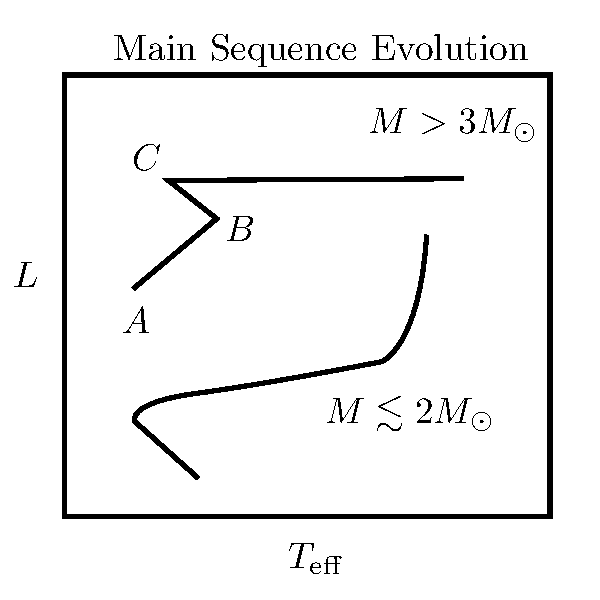
\includegraphics[width = 4in]{MSDiagram.pdf}
      \caption{Evolution of a massive star. From $A$ to $B$, the star
        is undergoing Main Sequence hydrogen burning. Temperature is
        increasing as $X$ is decreasing until finally all hydrogen is
        depleted in the core. From $B$ to $C$, the pure helium core
        undergoes Kelvin-Helmholtz contraction (this is called the
        ``Henyey Hook''). Beyond $C$, hydrogen is burning in a shell.}
      \label{fig:2}
    \end{figure}

    \n For stars less than $1.5\ M_\odot$, there is no abrupt transition
    (the Henyey Hook). Rather, it develops a growing (in mass) helium
    core. 

    \subsubsection{The Red Giant Branch (RGB)}
    \label{sec:red-giant-branch}

    For stars less than about $2\ M_\odot$, as the star leaves the
    main sequence, it travels horizontally on the HR diagram and
    eventually starts making its way back up the Hayashi track. This
    portion of the star's life is called the \textbf{Red Giant Branch}
    (RGB). After hydrogen is depleted in the core, hydrogen continues
    burning in a shell around the helium core. The radius of this core
    is much less than the radius of the star. When a one solar mass
    star ``leaves'' the main sequence, we typically have
    $M_{\mathrm{He}}=0.1 M_\odot$. However, the helium core, once
    degenerate, will \emph{decrease} in radius as the mass increases
    (where the mass gain is fueld by the hydrogen shell burning).\\
    
    \n Then the temperature in the shell is given by
    \begin{equation}
      \label{eq:240}
      kT_s\approx \frac{GM_c}{R_c}m_p
    \end{equation}
    for a shell where the pressure scale height is $R_c$. Now,
    assuming electron scattering sets the opacity, the luminoity is
    \begin{equation}
      \label{eq:241}
      L_{\mathrm{rad}}=4\pi R_c^2\left[\frac{1}{3}\frac{c}{\kappa\rho}\frac
{1}{R_c}aT_s^4\right]
    \end{equation}
    or more succinctly,
    \begin{equation}
      \label{eq:242}
      \boxed{L_{\mathrm{rad}}=\frac{4\pi}{3}\frac{R_c}{\kappa\rho_s}
acT_s^4}
    \end{equation}
    Now requiring that $L_{\mathrm{nuc}}=\varepsilon
    M_{\mathrm{shell}}=L_{\mathrm{rad}}$ actually tells us that at
    this stage, CNO burning dominates pp burning. Assuming again that
    the nitrogen proton scatter is the slow step, we get
    \begin{equation}
      \label{eq:243}
      \varepsilon_{\mathrm{CNO}}=6.6\times
      10^{24}\frac{\rho}{T_7^{2/3}}\exp\left(-70.7
        T_7^{-1/3}\right)=\varepsilon_0\rho T^\nu
    \end{equation}
    In this case, $\nu=24/T_7^{1/3}\sim 16$. Using this to find the
    density in the shell allows us to get the luminosity. The
    punchline is that 
    \begin{equation}
      \label{eq:244}
      \rho=\left[\frac{4}{3}\frac{\sigma T_5^{4-\nu}}
{\varepsilon_0R_c^2\kappa}\right]^{1/3}
    \end{equation}
    Then the luminosity scales as
    \begin{equation}
      \label{eq:245}
      L\propto R_c^{5/3}T_5^{(8+\nu)/3}
    \end{equation}
    But since $T_s\propto M_c/R_c$, we get
    \begin{equation}
      \label{eq:246}
      L\propto R_c^{-(1+\nu/3)}M_c^{(8+\nu)/3}
    \end{equation}
    Plugging in fiducial values for scaling relations gives us
    \begin{equation}
      \label{eq:247}
      L=5\times 10^{31}\ \mathrm{erg\ s^{-1}}\left(\frac{0.1R_\odot}{R}
\right)^{25/3}\left(\frac{M_c}{0.2M_\odot}\right)^{10}
    \end{equation}
    Since the helium core is degenerate, $R_c\propto M_c^{-1/3}$. This
    would make the mass dependence of $L$ even stronger. \\

%%%%%%%%%%%%%%%%%%%%%%%%%%%%%
% Monday, February 27, 2012 %
%%%%%%%%%%%%%%%%%%%%%%%%%%%%%
    \n \textit{Monday, February 27, 2012}

    \subsection{The Sch\"onberg-Chadrasekhar Limit}
    \label{sec:schonb-chadr-limit}

    Returning to stars with masses above around $6M_\odot$, where the
    hydrogen burning core ends, we have a substantial mass helium
    core. \figref{fig:3} shows how the hydrogen mass fraction evolves
    in the profile.\\

    \begin{figure}[h!]
      \centering
      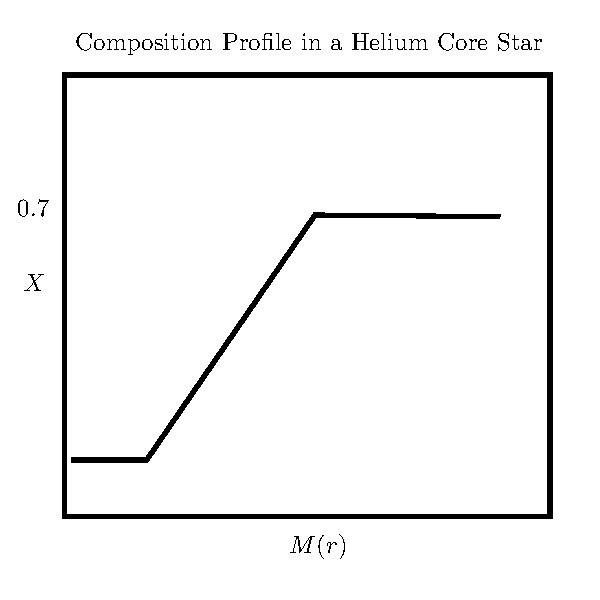
\includegraphics{compPlot.pdf}
      \caption{The composition profile of a star with a helium
        core. In the outer region, we still have $X\sim 0.7$ since
        that material is largely unburned.}
      \label{fig:3}
    \end{figure}
    \n This change in hydrogen mass fraction is the source of the
    ``Henyey Hook'' seen in large mass evolutionary trackds. After the
    hydrogen burning shell is extinguished undergoes Kelvin-Helmholtz
    contraction until the Helium ignites. This heilum core is nearly
    isothermal, so using hydrostatic equilibrium and the same old
    Virial theorem trick,
    \begin{equation}
      \label{eq:248}
      \frac{dP}{dr}=-\rho(r)\frac{Gm(r)}{r^2}
    \end{equation}
    Now multiplying both sides by $4\pi r^3$ and integrating, we get
    \begin{equation}
      \label{eq:234}
      \int_0^{R_c}4\pi r^3\frac{dP}{dr}dr=-G\int_0^{R_c}\frac{4\pi r^2m(r)
\rho(r)}{r}dr
    \end{equation}
    The term on the left is, integrating by parts,
    \begin{equation}
      \label{eq:249}
      \int_0^{R_c}4\pi r^3\frac{dP}{dr}dr=4\pi
      R_{\mathrm{core}}^3P_{\mathrm{core}}(R_{\mathrm{core}})-12\pi\int_0^
{R_c}r^2P(r)\,dr
    \end{equation}
    and the right side is roughly the gravitational potential, so
    \eqref{eq:234} becomes
    \begin{equation}
      \label{eq:250}
      4\pi
      R_{\mathrm{core}}^3P_{\mathrm{core}}(R_{\mathrm{core}})-12\pi\int_0^
{R_c}r^2P(r)\,dr=-\frac{GM_{\mathrm{core}}}{R_{\mathrm{core}}}
    \end{equation}
    Since we have
    $P(r)=\rho(r)kT_{\mathrm{core}}/(\mu_{\mathrm{core}}m_p)$. Then we
    can recast \eqref{eq:250} quite easily to
    \begin{equation}
      \label{eq:251}
      4\pi R_{\mathrm{core}}^3P_{\mathrm{core}}(R_{\mathrm{core}})-3\frac
{kT_{\mathrm{core}}}{mu_{\mathrm{core}}m_p}M_{\mathrm{core}}=-\frac{GM_
{\mathrm{core}}^2}{R_{\mathrm{core}}}
    \end{equation}
    Solving for the pressure, we have
    \begin{equation}
      \label{eq:252}
      P_{\mathrm{core}}(R_{\mathrm{core}})=\frac{3}{4\pi}\frac{kT_{\mathrm
{core}}}{\mu_{\mathrm{core}}m_p}\frac{M_{\mathrm{core}}}{R_{\mathrm{core}}
^3}-\frac{1}{4\pi}\frac{GM_{\mathrm{core}}^2}{R_{\mathrm{core}}}
    \end{equation}
    Note that this equation has a well-defined maximum at some
    critical core radius. The radius is
    \begin{equation}
      \label{eq:253}
      R_{\mathrm{core,
          max}}=\frac{GM_{\mathrm{core}}\mu_{\mathrm{core}}m_p}{k T_
{\mathrm{core}}}\frac{4}{9}
    \end{equation}
    and the maximum pressure is
    \begin{equation}
      \label{eq:254}
      P_{\mathrm{core,max}}=0.7\left(\frac{kT_{\mathrm{core}}}{\mu_{\mathrm
{core}}m_p}\right)^4\frac{1}{G^3 M_{\mathrm{core}}^2}
    \end{equation}
    The overlying envelope must exert a pressure
    \begin{equation}
      \label{eq:255}
      P_{\mathrm{base}}\sim\frac{GM^2}{R^4}
    \end{equation}
    At the interface between the pure helium core and the
    hydrogen/helium mix envelope, there must be a discontinuity in the
    density (like a water/air interface, sort of). The $R$ in
    \eqref{eq:255} is really just the scale height in the H/He
    envelope, so we will use
    \begin{equation}
      \label{eq:256}
      kT_{\mathrm{envelope}}\approx\frac{GM\mu_{\mathrm{envelope}}m_p}{R}
=kT_{\mathrm{core}}
    \end{equation}
    where we've mandated a contininous temperature profile at the
    interface. Then the pressure from the envelope is
    \begin{equation}
      \label{eq:257}
      P_{\mathrm{envelope}}=\frac{GM^2}{R^4}=\left(\frac{kT_{\mathrm
{core}}}{\mu_{\mathrm{envelope}}m_p}\right)^4\frac{1}{G^3m^2}
    \end{equation}
    assuming that $M\gg M_{\mathrm{core}}$. To have a valid solution,
    we require
    \begin{equation}
      \label{eq:258}
      0.68\frac{1}{\mu_{\mathrm{core}}^4}\frac{1}{M_{\mathrm{core}}}>\frac
{1}{\mu_{\mathrm{envelope}}}\frac{1}{M^2}
    \end{equation}
    So then the requirment on the core mass is
    \begin{equation}
      \label{eq:259}
      M_{\mathrm{core}}<M\left(\frac{\mu_{\mathrm{envelope}}}{\mu_{\mathrm
{core}}}\right)^2\alpha
    \end{equation}
    for some numerical constant $\alpha$. Noting that
    $\mu_{\mathrm{envelope}}=0.6$ and $\mu_{\mathrm{core}}=1.33$. The
    ``real'' result (not derived here) is
    \begin{equation}
      \label{eq:260}
      q_c=\frac{M_{\mathrm{core}}}{M}=0.37\left(\frac{\mu_{\mathrm
{envelope}}}{\mu_{\mathrm{core}}}\right)^2=0.08
    \end{equation}
    If $M_{\mathrm{core}}>0.08M$ \emph{and} the core is not
    degenerate, \emph{then} this core is not a solution to hydrostatic
    balance.\\

    \n Now what about electron degeneracy? In smaller stars, the core
    becomes degnerate before igniting helium. Then the equation of
    state becomes
    \begin{equation}
      \label{eq:261}
      P(r)=K_{\mathrm{NR}}\rho^{5/3}(r)
    \end{equation}
    And thus
    \begin{equation}
      \label{eq:262}
      P_{\mathrm{core}}(R_{\mathrm{core}})=\frac{K_{\mathrm{NR}}M^{5/3}}{R_
{\mathrm{core}}^5}-\frac{1}{4\pi}\frac{GM_{\mathrm{core}}^2}{R_{\mathrm
{core}}^4}
    \end{equation}
    Note that this pressure has \emph{no} maximum like the ideal gas
    situation. That is, the core mass can have any mass
    whatsoever. \figref{fig:4} shows how degeneracy affects different
    stars.\\

    \begin{figure}[h!]
      \centering
      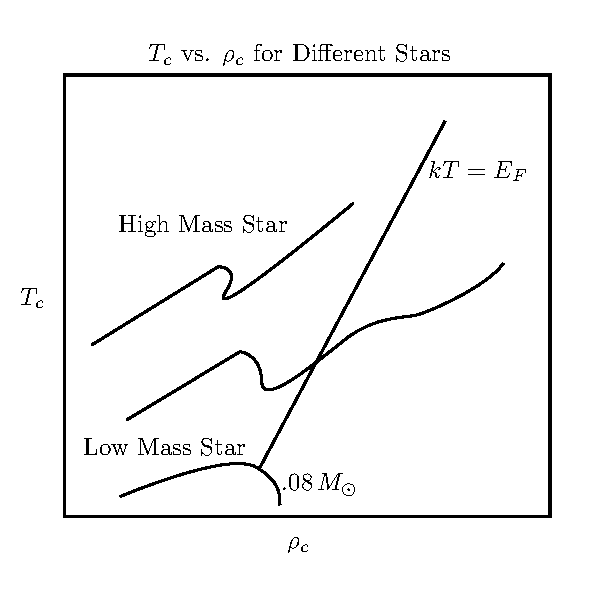
\includegraphics{TcRhoc.pdf}
      \caption{$T_c$ versus $\rho_c$ for various stars. High mass stars 
reach the helium ignition temperature before becoming degenerate, but lower 
mass stars do not, so they undergo a helium flash. A $0.08\,M_\odot$ star 
is shown, and barely (if ever) reaches hydrogen ignition.}
      \label{fig:4}
    \end{figure}
    
    \n Returning to the more massive stars, if
    $q_{\mathrm{core}}>0.08$ at the time of hydrogen core depletion,
    there is no isothermal solution and the star simply contracts on
    the Kelvin-Helmholtz timescale:
    \begin{equation}
      \label{eq:263}
      t\approx \frac{GM_{\mathrm{core}}^2/R_{\mathrm{core}}}{L}=10^6\ 
\mathrm{years}\left(\frac{6\,M_\odot}{M}\right)\left(\frac{5\,R_\odot}{R}
\right)
    \end{equation}
    So these stars contract very rapidly.\\
    
    \n Now consider stars in the range of $2\,M_\odot$ and
    $6\,M_\odot$. Initially, suppose $q<q_c$, but hydrogen shell
    burning occrs. Now $q$ will increase until $q>q_c$ and the core
    undergoes Kelvin-Helmholtz contraction. For stars with less than
    $2\,M_\odot$, the core will become degenerate before helium
    burning can star.\\

%%%%%%%%%%%%%%%%%%%%%%%%%%%%%%%%
% Wednesday, February 29, 2012 %
%%%%%%%%%%%%%%%%%%%%%%%%%%%%%%%%
    \n \textit{Monday, February 29, 2012}
    \subsection{Helium and Higher Burning}
    \label{sec:helium-burning}

    Helium burns in advanced stars via the triple-alpha process,
    according to
    \begin{align}
      \label{eq:264}
      \mathrm{{}^4He+{}^4He\to{}^8Be+\gamma}\\
    \end{align}
    However, $\mathrm{{}^8Be}$ is unstable with a decay time of around
    $\tau\sim 2\times 10^{-16}\ \mathrm{sec}$.  The Gamow energy for
    this interaction is $E_{\mathrm{G}}=31.4\ \mathrm{MeV}$, so the
    Gamow peak occurs at
    \begin{equation}
      \label{eq:265}
      E_0=\left(\frac{E_{\mathrm{G}}(kT)^2}{4}\right)=83\mathrm{keV}T_8^
{2/3}
    \end{equation}
    So once $T>8\times 10^7\ \mathrm{K}$ or so, the reaction to make
    $\mathrm{{}^8Be}$ proceeds rapidly and can achieve thermal and
    chemical equilibrium.\\

    \n Equating the chemical potentials, we have
    \begin{equation}
      \label{eq:266}
      \frac{n_8}{n_4^2}=2^{3/2}\left(\frac{h^2}{2\pi m_\alpha
          kT}\right)^{3/2}\exp\left(-\frac{m_8-2m_\alpha c^2}{kT}\right)
    \end{equation}
    Normalizing to $\rho=10^4\ \mathrm{g\,cm^{-3}}$ of pure helium (at
    the core, obviously), we get
    \begin{equation}
      \label{eq:267}
      \frac{n_8}{n_4}=3\times
      10^{-6}T_8^{-3/2}\left(\frac{\rho}{10^4\,\mathrm{g\,cm^{-3}}}\right)
\exp\left(-\frac{10.64}{T_8}\right) 
    \end{equation}
    At $T_8=2$, about 1 in $10^{-8}$ of the nuclei at any given time
    are ${}^8\mathrm{Be}$. Then another alpha particle can combine
    this a ${}^8\mathrm{Be}$ nucleus creating a ${}^{12}\mathrm{C}$
    nucleus. However, this is actually a carbon nucleus in an excited
    state of carbon that will eventually decay to the ground state
    through a strange prcess. First though, we note the Gamow energy
    and Gamow peak energy for the Carbon synthesis reaction:
    \begin{align}
      \label{eq:268}
      E_\mathrm{G}&=\left(\pi\alpha(2)(4)\right)^22m_rc^2=168\,\mathrm{MeV}
\\
      \label{eq:268a}
      E_0&=146\,\mathrm{keV}T_8^{2/3}
    \end{align}
    This is for the reaction
    \begin{equation}
      \label{eq:269}
      \mathrm{\alpha+{}^8Be\to{}^{12}C^*+\gamma}
    \end{equation}
    Now let us assume that the temperature is high enough so that the
    excited state of ${}^{12}\mathrm{C}$ becomes populated via a
    chemical equilibrium of \eqref{eq:269}. Now equating
    \textit{these} chemical potentials and noting that that of the Be
    isotope is just twice that of the alpha particles:
    \begin{equation}
      \label{eq:270}
      3\mu_4=\mu_{12^*}
    \end{equation}
    Messy algebra ensures, with the result that
    \begin{equation}
      \label{eq:271}
      \frac{n_{\mathrm{12^*}}}{n_4}=5\times
      10^{-10}\left(\frac{\rho}{10^5}\right)^2T_8^3\exp\left(-\frac{44}
{T_8}\right)
    \end{equation}
    Where we have implicitly used the binding energy of
    ${}^{12}\mathrm{C}^*$, which is $7.644\,\mathrm{MeV}$ (notably
    higher than that of the reactants, Be and the alpha particles, at
    $7.366\,\mathrm{MeV}$). Note that so far, this reaction has
    actually \emph{lost} energy. The only way this reaction provides
    energy is in the two decays it takes for ${}^{12}\mathrm{C}^*$ to
    get down to the ground state of Carbon. For these decays, we have
    \begin{equation}
      \label{eq:272}
      \Gamma_{\mathrm{rad}}=3.67\,\mathrm{MeV}
    \end{equation}
    and thus the decay rate is
    \begin{equation}
      \label{eq:273}
      r=\frac{\Gamma}{\hbar}=5.5 \times 10^{12}\,\mathrm{s^{-1}}
    \end{equation}
    Putting all of this together, we have that the nuclear energy
    generation rate is
    \begin{equation}
      \label{eq:274}
      \varepsilon = \frac{n_{12^*}E}{\tau}\frac{1}{\rho}=5.3\times 10^
{21}\mathrm{erg\,g^{-1}\,s^{-1}}\rho_5^2T_8^{-3}\exp\left(-\frac{44}
{T_8}\right)
    \end{equation}
    In order to determine this, we had to know the mass difference
    between ${}^{12}C^*$ and three alpha particle, as well as the
    photon decay rate of ${}^{12}C^*$ into plain old
    $^{12}\mathrm{C}$. Note that this reaction is even more
    temperature sensitive than either hydrogen burning source, and the
    energy per reaction per nucleon is about a tenth of what it is for
    hydrogen burning. Thus, we expect helium burning to end much
    faster than hydrogen burning since more reactions have to happen
    per unit time to match the luminosity, \emph{and} the luminosity
    is higher due to the change in composition that we found earlier.\\
    
    \subsubsection{Higher Burning}
    \label{sec:higher-burning-1}

    Once carbon is present in the core, it can burn to oxygen by the
    synthesis of an alpha particle and a carbon nucleus. Similarly,
    the Oxygen can be burned to Neon. The relevant values are shown in
    Table \ref{tab:1}
    \begin{table}[h!]
      \centering
      \begin{tabular}{l c c}
        Reaction & $E_0(T_8=2)$ &
        $\exp\left[-3\left(\frac{E_\mathrm{G}}{4kT}\right)^{1/2}\right]$\\
        \hline\hline
        $\alpha+{}^{12}\mathrm{C}$ & 315 keV & $1.3\times 10^{-24}$\\
        $\alpha+{}^{16}\mathrm{O}$ & 390 keV & $5.5\times 10^{-38}$\\
        $\alpha+{}^{20}\mathrm{Ne}$& 460 keV & $1.5\times 10^{-44}$
      \end{tabular}
      \caption{Parameters controlling the burning of carbon, oxygen, and 
neon.}
      \label{tab:1}
    \end{table}
    The first reaction in Table \ref{tab:1} does occur fast enough to
    compete with the triple alpha process, so advanced stars typically
    have a core consisting of both carbon and oxygen.

    \subsubsection{Helium Burning in a Massive Star}
    \label{sec:heli-burn-mass}
    In a convective core, helium burning starts at
    $T=10^8\,\mathrm{K}$ due to the high temperature sensitivity of
    the triple alpha process. Now recall that the luminosity of an
    evolved star is higher than it was as a ZAMS star, so the burn
    time is
    \begin{equation}
      \label{eq:276}
      t_{\mathrm{He\,burn}}=\frac{E_{\mathrm{nuc}}M_{\mathrm{burn}}}{L}
    \end{equation}
    which is shorter than the hydrogen-burning main sequence burn
    time. For stars above around $6\ M_\odot$, carbon burning will
    eventually occur, and as we move on up to higher and higher
    masses, more and more heavy elements will get their turn at
    burning, with the most massive stars stopping at Fe/Si burning
    (since the binding energy per nucelon peaks there).\\

    \n For stars greater than around $2 M_\odot$, the helium ignites
    when the electron gas in the core is nondegnenerate. Solar mass
    stars, however, are not so lucky.

    \subsubsection{Helium Core Flash}
    \label{sec:helium-core-flash}

    For stars with masses less than around $2\,M_\odot$, the helium
    cores have degenerate electrons. Meanwhile, the CN cycle burning
    increase the mass of the He core. Before we delve into the details
    of the dynamics of the degenerate core, here's a quick refresher
    of degeneracy.\\

    \n The DeBroglie wavelength of particles in a gas of temperature
    $T$ is

    \begin{equation}
      \label{eq:277}
      \lambda=\frac{h}{p}=\frac{h}{\sqrt{mkT}}
    \end{equation}
    The quantum mechanics impacts the equation of state when $\lambda
    \gtrsim n^{-1/3}$. Then the condition becomes
    \begin{equation}
      \label{eq:278}
      n^{1/3}>\frac{\sqrt{mkT}}{h}
    \end{equation}
    Note that this is the quantum concentration found in our previous
    discussion of the Saha equation. And so $n^{2/3}\propto T$. As
    $T\to 0$, then the DeBroglie wavelenth is going to $\lambda\propto
    n^{1/3}$ since they are degenerate and that is necessarily the
    separation distance. Now the pressure for a nonrelativistic gas is
    given by
    \begin{equation}
      \label{eq:279}
      P=\frac{2}{3}E
    \end{equation}
    where $E$ is the energy density. The energy is primarily in
    kinetic energy,
    \begin{equation}
      \label{eq:280}
      E_k=\frac{p^2}{2m_e}=\frac{(\hbar n_e^{1/3})^2}{2m_e}
    \end{equation}
    So the Fermi energy follows $E_F\propto \rho^{2/3}$, and so the
    presure is $P=\rho E_f\propto \rho^{5/3}$. For hydrostatics, we
    have
    \begin{equation}
      \label{eq:281}
      P=\frac{GM^2}{R^4}\propto
      \left(\frac{M}{R^3}\right)^{5/3}\quad\Rightarrow \quad R\propto M^
{-1/3}
    \end{equation} 
    Thus more massive degenerate objects have \emph{smaller}
    radii.\\   
%%%%%%%%%%%%%%%%%%%%%%%%%
% Friday, March 2, 2012 %
%%%%%%%%%%%%%%%%%%%%%%%%%
  
    \n \textit{Friday, March 2, 2012}\\

    \n Now returning to our intermediate mass star with a helium
    core, the temperature in the hydrogen burning shell located at
    about $R_c$ (the radius of the core) is
    \begin{equation}
      \label{eq:282}
      kT_s\approx\frac{G M_sm_p}{\mu_e R_c}\quad\Rightarrow \quad
      T_S\propto \frac{M_c}{R_c}\propto M_c^{4/3}
    \end{equation}
    So as the shell deposits more and more helium into the core, the
    temperature on the outer edge is rising in time. In the degenerate 
core,
    the dominant form of heat transport is electron conduction from
    electron scattering off of the ions. This mode is so efficient
    that the core is nearly isothermal (though it's actually a bit
    hotter out towards the hydrogen burning shell since neutrino
    cooling is lowering the temperature at the center).\\

    \n When the star is in hydrostatic balance and has an ideal gas
    equation of state, an injection of entropy would lead to a
    temperature (negative heat capacity). For a star, this means that
    the pressure drops when entropy is added. Here are some ways to
    cause trouble in such a star:
    \begin{itemize}
    \item Make the electrons degenerate so that the pressure is
      independent of temperature. 
    \item Thin Shell Instability
    \end{itemize}
    The \textbf{Thin Shell Instability} was discovered in 1965 and is
    a thermonuclear instability that occurs when temperature sensitive
    burning is in a geometrically thin shell. By ``geometrically
    thin'', we mean that at the location of the shell, $\Delta r\ll
    R$. To get a better handle on this mechanism, recall the condition
    for hydrostatic balance (again):
    \begin{equation}
      \label{eq:283}
      \frac{dP}{dr}=-\rho(r)\frac{GM(r)}{r^2}
    \end{equation}
    Integrating this over a thin shell gives us the plane-parallel
    atmosphere result:
    \begin{equation}
      \label{eq:284}
      \int_{P_{\mathrm{sh}}}^0dP=-\int_{R_{\mathrm{sh}}}^\infty
      \frac{GM(r) \rho(r)}{r^2}dr
    \end{equation}
    Or, switching to the mass coordinate,
    \begin{equation}
      \label{eq:285}
      P_{\mathrm{sh}}=\int_m^M\frac{Gm(r)}{4\pi r^4}dm=\frac{G
        M_{\mathrm{sh}}}{R_{\mathrm{sh}}^2}\frac{\Delta m}{4\pi R_{\mathrm
{sh}}^2}
    \end{equation}
    where $dm=4\pi r^2 \rho(r)\,dr$ and $\Delta m= M-m$, which is
    the mass in the shell (approximately, since we are ignoring the
    contribution of the envelope).\\

    \n When the pressure is constant, 
    \begin{equation}
      \label{eq:286}
      T\frac{ds}{dt}=c_P\frac{dT}{dt}=\varepsilon-\frac{1}{\rho}\bm{\nabla}
\cdot\mathbf{F}
    \end{equation}
    Then this becomes positive, hence the instability (heat capacity
    has become positive). The flux term, from radiative diffusion, is
    \begin{equation}
      \label{eq:287}
      \frac{1}{\rho}\bm{\nabla}\cdot\mathbf{F}=\frac{1}{dy}\frac{c}
{3\kappa}\frac{d}{dy}aT^4\propto
      \frac{ac T^4}{3\kappa y^2}
    \end{equation}
    where $y$ is the column depth introduced earlier, $y=\int
    \rho(r)\,dr$, of the shell. So then \eqref{eq:287} becomes
    \begin{equation}
      \label{eq:288}
      c_P\frac{dT}{dt}=\varepsilon-\frac{acT^4}{3\kappa y^2}
    \end{equation}
    For most nuclear energy generation rates, $\varepsilon\propto
    T^\nu$ with $\nu \gg 4$, so this becomes highly unstable. This
    occurs in stellar evolution as the helium shell flashed in
    asymptotic giant branch (AGB) stars. A limit cycle can be formed
    where a thin shell piles up until it burns unstably, starting the
    process over again. In an accretion context, white dwwarfs accrete
    hydrogen in a thin shell and burn unstably, which is a
    \textbf{Classical Nova}. They can also do this with helium, which
    causes a larger nova or \textbf{.Ia} explosion. Neutron stars
    accrete hydrogen and burn to make a \textbf{Type I X-Ray Burst}
    (hydrogen burns to helium, helium burns to carbon and
    oxygen). Additionally, this process can fuel superbursts, where
    carbon is burned to heavy elements.\\

    \n Returning to the degenerate electron source of instability,
    an extremely degenerate electron gas can be the cause of unstable
    burning. In this regime, the pressure is insensitive to the
    temperature, so the pressue is constant. The same equation that
    was releven to the thin shell instability applies:
    \begin{equation}
      \label{eq:289}
      c_P\frac{dT}{dt}=\varepsilon-\frac{dL(r)}{dm(r)}
    \end{equation}
    but the reason that $c_P$ is positive is now different (degeneracy
    versus plane-parallel). Due to the fact that the temperature in
    the core isn't monotonic, helium ignition starts off-center
    (remember, the neutrino cooling keeps the center of the core
    cooler than surrounding areas). In a 1-D model, a convective zone
    forms at the ignition point. The temperature continues to rise
    until such a time where the degeneracy is broken and the shell
    isn't geometrically thin. At this degeneracy breaking-point, we
    have $kT\sim E_F$. The Fermi energy follows the virial form,
    \begin{equation}
      \label{eq:290}
      E_F\sim \frac{G M_c}{R_c}m_{\mathrm{He}}\sim kT
    \end{equation}
    At this point, the scale height will now be of the order of the
    radius of the star, so it is \emph{not} geometrically thin. Then
    the heat capacity returns to being negative, ending the unstable
    burning. After this event has passed, degeneracy in the local area
    has been lifted. A succession of flashes follows, slowly removing
    the degeneracy and paving the way for stable ``main sequence''
    helium burning.

    \subsection{The Horizontal Branch and The Asymptotic Giant Branch}
    \label{sec:horizontal-branch}

    The core flash lifts degeneracy, leaving behind a nondegenerate
    helium-burning star. Recalling that $L\propto \mu^4$, the
    luminosity increases dramatically ($L_\odot\to 10L_\odot$). Once
    the core flash is over, we would expect stellar evolution to slow
    down or stop due to the stable nature of helium core
    burning. The envelope is expanded by a large factor, eseentially
    shutting off the hydrogen shell burning. The luminosity then
    decreasese quickly, creating a tip on an HR diagram (called the
    tip of the red giant branch, or TRGB). Kelvin-Helmholtz
    contraction occurs until stable helium core burning is occuring at
    a rate that balances radiative losses. Essentially the star has
    become a helium-burning main sequence star, often called a
    \textbf{Red Clump} star. If the star loses part or all of its
    hydrogen shell, the luminosity is unaffected, but the radius
    obviously does, so there is a range of colors of red clump stars,
    depending on how much hydrogen they have retained, forming the
    \textbf{Horizontal Branch} on the HR diagram.\\

    \n The helium core burning lifetime is somewhere around 65-100
    million years. This is shorter than the hydrogen burning main
    sequence since the triple alpha process is less efficient in
    energy generation \emph{and} the luminosity is greater. After the
    helium core is spent, there is a carbon/oxygen core and the star
    with masses between 2 and 6 $M_\odot$ ascend up the
    \textbf{Asymptotic Giant Branch} (AGB), where only hydrogen and helium
    shell burning can power them. A series of helium shell flashes
    occur, but they never get hot enough to ignite
    carbon, so will ened their lives as C/O white dwarfs.\\

    \n Stars traveling up the AGB will have a stable hydrogen burning
    shell dumping helium onto an unstable helium burning shell. That
    is, the rate of helium supplied by the hydrogen shell cannot be
    the rate at which helium stably burns in the helium shell. There
    is a net increase of mass entering the core,
    $\dot{M}_{\mathrm{in}}$. Additionally, the weakly bound envelope
    is losing mass due to a wind taking mass to infinity,
    $\dot{M}_{\mathrm{wind}}$. In the end, mass loss wins the game,
    and the degenerate core is left behind as a white dwarf, with most
    of the envelope mass lost into a nebula.\\

%%%%%%%%%%%%%%%%%%%%%%%%%
% Monday, March 5, 2012 %
%%%%%%%%%%%%%%%%%%%%%%%%%
    \n\textit{Monday, March 5, 2012}

    \section{White Dwarfs}
    \label{sec:endp-stell-evol}

    \subsection{The Physics of Degenerate Objects and the
      Chandrasekhar Mass}
    \label{sec:white-dwarf-cooling}

    At the late stages of stellar eolution, the electrons become more
    and more degenerate, eventually dominating the pressure. We now
    work out the resulting $M(R)$ relation in this limit. The equation
    of state is just
    \begin{equation}
      \label{eq:317}
      n_e=\frac{2}{h^3}\int_0^{p_F} 4\pi p^2\,dp=\frac{8\pi}{3h^3}p_F^3
    \end{equation}
    in the fully degenerate limit (that is, electrons are filling all
    of momentum space up to the Fermi momentum of the gas). Then the
    pressure is just (as derived earlier)
    \begin{equation}
      \label{eq:318}
      P_e=\frac{2}{5}n_e E_F
    \end{equation}
    when things are non-relativistic as we presume for now. Expanding
    out \eqref{eq:318}, we get
    \begin{equation}
      \label{eq:319}
      P=\frac{2}{5}n_e\frac{1}{2 m_e}p_F^2=\frac{n_e}{5
        m_e}\left(\frac{3h^3n_e}{8\pi}\right)^{2/3}=n_e^{5/3}\left(\frac
{3h^2}{8\pi}\right)^{2/3}\frac{1}{5 m_e}
    \end{equation}
    If we typically have $\rho=A m_pn_i$ and $n_e=Zn_i$, so that
    \begin{equation}
      \label{eq:320}
      n_e=Z\frac{\rho}{Am_p}\approx \frac{\rho}{2m_p}\qquad
      \textrm{(where $A=2Z$)}
    \end{equation}
    Then the pressure is
    \begin{equation}
      \label{eq:321}
      P=\left(\frac{\rho}{2m_p}\right)^{5/3}\left(\frac{3h^3}{8\pi}\right)^
{2/3}\frac{1}{5 m_e}
    \end{equation}
    Now, let's just ask what the rough properties are of an object
    supported by degenerate electrons. Yet agin, let's just write the
    pressure as
    \begin{equation}
      \label{eq:322}
      \frac{dP}{dr}=-\rho\frac{Gm(r)}{r^2}\quad\Rightarrow\quad P\sim G
\frac{M}{R^2}\frac{M}{R^2}=\frac{GM^2}{R^4}
    \end{equation}
    But now let's set $\rho R^3=M$, or equivalently,
    $R=(M/\rho)^{1/3}$ to eliminate the radius from the pressure. Then
    linking the pressures from hydrostatic balance and degeneracy
    pressure, we get
    \begin{equation}
      \label{eq:323}
      P_c\sim\frac{GM^2}{M^{4/3}}\rho^{4/3}=\frac{1}{5m_e}\left(\frac{\rho}
{2m_p}\right)^{5/3}\left(\frac{3h^3}{8\pi}\right)^{2/3}
    \end{equation}
    Solving this for the density gives
    \begin{equation}
      \label{eq:324}
      \rho\sim 4\times 10^5\,\mathrm{g\,cm^{-3}}\left(\frac{M}{0.1\,M_
\odot}\right)^2\left(\frac{m_x}{m_e}\right)^3
    \end{equation}
    where $m_x$ is presumably the mass of the degenerate particle (in
    our case, the electron mass).Now this is the crude scaling at low 
masses and it is important to
    ask what happens as the mass increases. according to our relation,
    the density increases. We can get the radius as well from the
    density, so
    \begin{equation}
      \label{eq:325}
      R\sim 8\times 10^8\,\mathrm{cm}\left(\frac{0.1\,M_\odot}{M}\right)^
{1/3}\left(\frac{m_e}{m_x}\right)
    \end{equation}
    So the star gets smaller as the mass increases. Note that the more
    proper formula is
    \begin{equation}
      \label{eq:326}
      R=2\times 10^9\,\mathrm{cm}\left(\frac{0.1\,M_\odot}{M}\right)^
{1/3}\left(\frac{m_e}{m_x}\right)
    \end{equation}
    So for for a neutron star ($m_x\approx m_p$) we find $R\approx
    10^6\,\mathrm{cm}=10\,\mathrm{km}$.\\

    \n Anyway, returning to white dwarfs, as the mass increases,
    eventually the electrons start to become relativistic. In
    particular, we can just ask when the Fermi momentum is just the
    mass times the speed of light, $p_F\approx m_ec$, which means
    \begin{equation}
      \label{eq:327}
      m_ec=p_F=\left(\frac{3h^3n_e}{8\pi}\right)^{1/3}=\left(\frac
{3h^3\rho}{2m_p8\pi}\right)^{1/3}
    \end{equation}
    Solving \eqref{eq:327} for the density gives us
    \begin{equation}
      \label{eq:328}
      \rho= (m_e c)^3\frac{2m_p 8\pi}{3 h^3}\approx \frac{16
        \pi}{3}m_p\left(\frac{m_e c}{h}\right)^3
    \end{equation}
    Where we have phrased this in a suggestive way, noting that the De
    Broglie wavelength in the relativistic limit is
    $\lambda_c=h/(m_ec)$. This implies that the density reaches a
    critical level that is independent of any parameter:
    \begin{equation}
      \label{eq:329}
      \boxed{\rho_{\mathrm{crit}}=2\times 10^6\,\mathrm{g\,cm^{-3}}}
    \end{equation}
    So at these densities, things get weird. The first important point
    is that the relativistic gas we know of will be unstable and thus
    it is impossible to build such an object. In the extreme
    relativistic limit, the electron gass pressure is
    \begin{equation}
      \label{eq:330}
      P=\frac{1}{4}n_e E_F=\frac{1}{4}n_e p_F c=\frac{1}{4} n_ec\left(\frac
{3h^3n_e}{8\pi}\right)^{1/3}=n_e^{4/3}\frac{c}{4}\left(\frac{3h^3}{8\pi}
\right)^{1/3}
    \end{equation}
    Relating this to our hydrostatic approximation for the central
    pressure, we find
    \begin{equation}
      \label{eq:331}
      M^{2/3}=\frac{1}{G}\frac{c}{4}\frac{1}{(2m_p)^{4/3}}\left(\frac{3h^3}
{8\pi}\right)^{1/3}
    \end{equation}
    Which predicts a characteristic mass of such objects of
    \begin{equation}
      \label{eq:332}
      M+\frac{1}{G^{3/2}}\left(\frac{c}{4}\right)^{3/2}\frac{1}{(2m_p)
^2}\left(\frac{3h^3}{8\pi}\right)^{1/2}
      \approx 0.3 M_\odot
    \end{equation}
    In reality, the properly detailed calculation using the polytropic
    relations puts in new factors giving the proper
    \textbf{Chandrasekhar Mass}:
    \begin{equation}
      \label{eq:333}
      \boxed{M_{\mathrm{Ch}}=1.456\left(\frac{2}{\mu_e}\right)^2\,M_\odot}
    \end{equation}
    Where $\mu_e$ is, as always, the number of baryons per electron.
    If the star gets heavier than this mass, it undergoes catastrophic
    collapse, the outcome of which most likely depends on the (GARBLED
    TEXT (possibly the contents of the atmosphere?))

    \subsection{White Dwarf Cooling}
    \label{sec:white-dwarf-cooling}
    The white dwarf is ``burn'' hot, with $T\approx 2\times
    10^8\,\mathrm{K}$ or so, with the interior being completely
    isothermal due to the efficient conductive heat transfer of the
    degenerate electrons. There is some transition point at $E_F=kT$
    which gives a bottom boundary condition of degeneracy. Looking at
    the Fermi Energy,
    \begin{equation}
      \label{eq:334}
      E_F=\frac{1}{2m_e}\left(\frac{3h^3\rho}{8\pi
          2m_p}\right)^{2/3}=16\,\mathrm{eV}\,\rho^{2/3} =k T\quad
      \Rightarrow \quad 8625 T_8=16\rho^{2/3}
    \end{equation}
    So the transition density is
    \begin{equation}
      \label{eq:335}
      \rho_{\mathrm{tr}}=1.2\times 10^4\,\mathrm{g\,cm^{-3}}T_8^{3/2}
    \end{equation}
    \n In the outer, non degenerate layer of the white dwarf, the
    material is geometrically thin and $M_{\mathrm{outer}}\ll
    M$. Thus, the plane-parallel atmosphere precription is valid. The
    surface gravity for a typical white dwarf is
    \begin{equation}
      \label{eq:291}
      g=\frac{GM}{R^2}=1.6\times 10^8\,\mathrm{cm\,s^{-2}}
    \end{equation}
    where we have assumed $R=7\times 10^8\,\mathrm{cm}$ and
    $M=0.6\,M_\odot$. Then the pressure is
    \begin{equation}
      \label{eq:292}
      P=g\frac{\Delta m}{4\pi R^2}=\frac{\rho kT}{\mu m_p}
    \end{equation}
    With this, we can calculate where the electrons become
    degenerate. We find
    \begin{equation}
      \label{eq:293}
      \Delta M=10^{-3}M_\odot T_8^{5/2}
    \end{equation}
    In the hydrogen and helium layer. Now assuming that the flux is
    constant, and that the opacity follows a Kramers' Law form,
    \begin{equation}
      \label{eq:294}
      F=\mathrm{const}=\frac{1}{3}\frac{c}{\kappa\rho}\frac{d}{dr}\left
(aT^4\right)
    \end{equation}
    or
    \begin{equation}
      \label{eq:295}
      \frac{3F\kappa}{c}=\frac{d}{dy}aT^4
    \end{equation}
    Reintroducing the pressure, we get
    \begin{equation}
      \label{eq:296}
      \left[\frac{3F}{4c}\kappa_0\frac{\mu m_p}{k g}\frac{1}{a}\right]P
\,dP=T^{7.5}\,dT
    \end{equation}
    Now integrating this from the point where electrons are degenerate
    out to the surface, we get
    \begin{equation}
      \label{eq:297}
      \frac{L}{4\pi R^2}\frac{R^2}{GM}=\frac{F}{g}=\frac{2
        T_8^{8.5}}{8.5 P^2}\frac{4c k a}{3 \kappa_0 \mu m_p}
    \end{equation}
    Solving for the luminosity and scaling, we find
    \begin{equation}
      \label{eq:298}
      \boxed{L=2.5\,L_\odot \left(\frac{M}{0.6\,M_\odot
          }\right)\left(\frac{T_c}{10^8 \,\mathrm{K}}\right)^{7/2}}
    \end{equation}
    This is known as \textbf{Mestel's Cooling Law}, though it isn't
    really accurate, since the opacity is changing as we get towards
    the degeneracy. Now all of the energy source is coming from the
    thermal content of the ions, which is approximately
    \begin{equation}
      \label{eq:299}
      E_{\mathrm{th}}=\frac{3}{2}N_i k T=1.25\times 10^{48}\,\mathrm{ergs}
\left(\frac{M}{0.6\,M_\odot}\right)T_8
    \end{equation}
    Since the ions form an ideal gas. The luminosity is then obviously
    \begin{equation}
      \label{eq:300}
      L=-\frac{d}{dt}E_{\mathrm{th}}
    \end{equation}
    Note that the mass dependence cancels here. This gives us a
    differential equation:
    \begin{equation}
      \label{eq:301}
      \frac{T_8^{7/2}}{\tau}=-\frac{dT_8}{dt}
    \end{equation}
    where $\tau=4\times 10^{6}\,\mathrm{yrs}$. If we ignore $t\gg
    \tau$, this gives
    \begin{equation}
      \label{eq:302}
      T_8=\left(\frac{2}{5}\frac{\tau}{t}\right)^{2/5}
    \end{equation}
    Or more explicitly,
    \begin{equation}
      \label{eq:303}
      T_8=\left(\frac{1.6\times 10^6\,\mathrm{yrs}}{t}\right)^{2/5}
    \end{equation}
    Note that this solution is not valid at early time since we have
    ignored the initial data, however after a million years or so, the
    initial conditions are effectively forgotten anyway. Since we can
    find the central temperature from the mass and luminosity, we need
    only the mass and luminosity to determine a white dwarf's age.\\

    \n We must get the mass through a measure of $\log g$ through the
    spectrum. At higher gravity, we have
    \begin{equation}
      P_{\mathrm{ph}}=\frac{g}{\kappa}=\frac{\rho kT}{\mu m_p}\label{eq:
304}
    \end{equation}
    So as the density goes up, the gravity goes up (and thus the mass
    goes up). And indeed, as the
    pressure increases, the line widths in a spectrum increase. This
    phenomenon is called \textbf{Pressure Broadening}. \\

    \n There are some caveats to this theory, though. Primarily, we
    have ignored that ions do interact via Coulomb physics. We
    typically have 
    \begin{equation}
      \label{eq:305}
      \frac{e^2}{\avg{r}}\gtrsim kT
    \end{equation}
    Then we have
    \begin{equation}
      \label{eq:306}
      \Gamma = \frac{Z^2 e^2}{a kT}
    \end{equation}
    where $a$ is the average ion spacing. When $\Gamma>1$, ions
    interact strongly via Coulomb interactions. \\

    \n When in a Coulomb solid, $E_{\mathrm{th}}=3kT$, since each
    positional degree of freedom now has an energy. This phase
    transition introduces a latent heat. The WD goes crystalline at
    $\Gamma\approx 173$. In a Coulomb liquid, we have short-range
    order at $\Gamma\sim1$ and $C_V$ increases relative to
    $\frac{3}{2}N_i kT$. Lindimann in the 1920's discovered the
    following rule: when the average displacement at a given site in a
    lattice is bigeer than $0.1a$, the solid melts.\\
%%%%%%%%%%%%%%%%%%%%%%%%%%%%
% Wednesday, March 7, 2012 %
%%%%%%%%%%%%%%%%%%%%%%%%%%%%

    \n \textit{Wednesday, March 7, 2012}
    \subsection{Evolution of Larger Stars}
    \label{sec:evolution-gt-6}
    In stars larger than about 6 $M_\odot$, helium is ignited while
    the core is non degenerate. There is complete helium burning into
    a carbon/oxygen core. After that, carbon begins burning to
    magnesium via
    \begin{align}
      \label{eq:336}
      \mathrm{{}^{12}C+{}^{12}C}&\to \mathrm{{}^{24}Mg}\\
      &\to \mathrm{\alpha+{}^{20}Ne}\\
      &\to \mathrm{p+{}^{23}Na}\\
      &\to \mathrm{n+{}^{23}Mg}
    \end{align}
    Note that for heilum burning to take place, we needed a
    temperature of about $T=2\times 10^8\,\mathrm{K}$. The Coulomb
    barrier for the double carbon ignition will require a higher
    temperature than helium burning did, but these stars do ge hot
    enough for this to occur. 

    \subsubsection{Onset of Neutrino Emission}
    \label{sec:onset-neutr-emiss}

    These stars, since they are massive enough, gain an additional
    means of cooling (rather than radiative diffusion): neutrino
    cooling. Remember our equation of stellar structure
    \begin{align}
      \label{eq:337}
      T\frac{ds}{dt}=\varepsilon_{\mathrm{nuc}}-\frac{dL(r)}{dm(r)}-
\varepsilon_\nu
    \end{align}
    where $\varepsilon_\nu$ is the power emitted by the parcel of
    fluid as neutrinos that leave the star. Since the material in the
    star is optically thin to neutrinos, their is no transport
    problem, and so the local rate enters into the entropy equation
    (i.e., surface conditions are irrelevant, unlinke the situation
    with radiative diffusion).\\

    \n Now if we have $\varepsilon_\nu\gg dL(r)/dm(r)$, then the time
    scale for stellar evolution gets set by $\varepsilon_\nu$ rather
    than the photon luminosity!\\

    \n The cross section for neutrinos is approximately
    \begin{align}
      \label{eq:338}
      \sigma_\nu\sim 10^{-44}\,\mathrm{cm^2}\left(\frac{E_\nu}{\mathrm
{MeV}}\right)^2
    \end{align}
    So we're interested in when
    \begin{equation}
      \label{eq:339}
      \frac{M}{m_pR^2}\sigma_\nu>1
    \end{equation}
    It turns out that this condition is equivalient to
    \begin{equation}
      \label{eq:341}
      R<30\,\mathrm{km}\left(\frac{E_\nu}{\mathrm{MeV}}\right)
    \end{equation}
    Interestingly, neutron stars follow this criterion \emph{and} they
    are optically thick to neutrinos, so you will often hear in the
    lecture about the ``neutrinosphere'' on neutron star. Stars are
    not this dense at this stage, though.\\

    \n How are neutrnos created, though? The primary source is through
    positron-electron annihilation:
    \begin{equation}
      \label{eq:342}
      e^++e^-\to\nu_e+\overline{\nu}_e
    \end{equation}
    The temperature and density do get high enough at late times that
    there is a population of positrons where
    \begin{equation}
      \label{eq:343}
      \frac{e^++d^-\to \nu_e+\overline{\nu}_e}{e^++e^-\to 2\gamma}\sim 10^
{-19}
    \end{equation}
    It is of interest, then, to calculate the equilibrium abundance of
    positrons from
    \begin{equation}
      \label{eq:344}
      e^++e^-\to 2\gamma
    \end{equation}
    by equating the chemical potentials:
    \begin{equation}
      \label{eq:345}
      \mu_{e^+}+\mu_{e-}=0
    \end{equation}
    The chemical potentials are given by the usual formula (see Section
    \ref{sec:state-stell-inter}) and we get
    \begin{equation}
      \label{eq:346}
      n_{e^+}=g_e^2n_{e,Q}^2\frac{1}{n_e}\exp\left(-\frac{2m_e c^2}{kT}
\right)
    \end{equation}
    Scaling this result, we get
    \begin{equation}
      \label{eq:347}
      n_{e+}=7.7\times 10^{30}\left(\frac{10^4}{\rho}\right)T_9^3\exp\left
(-\frac{11.84}{T_9}\right)
    \end{equation}
    \begin{table}[h]
      \centering
      \begin{tabular}{c c}
        $T_9$ & $n_{e+}/n_{e^-}$\\
        \hline \hline
        1 & 0.02\\
        2 & >1
      \end{tabular}
      \caption{Relative densities of positrons and electrons at various 
temperatures}
      \label{tab:positron}
    \end{table}
    In the second entry in Table \ref{tab:positron}, the density of
    the electrons are set positrons rather than the ions, so our
    previous considerations are invalid. When does this happen?
    I.e., when does $n_{e^+}=n_e=Zn_i$? Well, it's when this
    happens:
    \begin{equation}
      \label{eq:348}
      \rho_4^2=2566 T_9^3\exp\left(-\frac{11.84}{T_9}\right)
    \end{equation}
    Which is satisfied at $\rho_4=1$ and $T_9=1.35$. Going back to
    our ``Saha'' equation, 
    \begin{equation}
      \label{eq:349}
      n_{e^+}n_{e^-}=4\left(\frac{2\pi m_e kT}{h^3}\right)^3\exp\left(-
\frac{2m_ec^2}{kT}\right)
    \end{equation}
    And so the rate of energy from neutrinos is
    \begin{equation}
      \label{eq:350}
      \frac{dU_\nu}{dt}=n_{e^+}n_{e^-}\avg{\sigma v}W
    \end{equation}
    where $\avg{\sigma v}$ is the ``reaction rate'' and $W$ is the
    energy loss from a pair of neutrinos leaving. Writing out the
    cross section of the neutrinos again,
    \begin{equation}
      \label{eq:351}
      \sigma = 1.4\times 10^{-45}\frac{c}{v}\left[\left(\frac{W}
{m_ec^2}\right)^2-1\right]\,\mathrm{cm^2}
    \end{equation}
    Thus $\avg{\sigma v}$ is just a constant:
    \begin{equation}
      \label{eq:352}
      \avg{\sigma v}=4\times 10^{-45}c
    \end{equation}
    Then the cooling rate is, more explicitly
    \begin{equation}
      \label{eq:353}
      \frac{dU_\nu}{dt}=5\times 10^{18}T_9^3\exp\left(-\frac{11.84}
{T_9}\right)\mathrm{erg\,cm^{-3}\,s^{-1}}
    \end{equation}
    Since the thermal energy is just
    \begin{equation}
      \label{eq:354}
      E_{\mathrm{th}}=nkT=7\times 10^{19}\,\mathrm{erg\,cm^{-3}}\,T_9\rho^4
    \end{equation}
    and thus the cooling timescale is
    \begin{equation}
      \label{eq:355}
      t_{\mathrm{cool}}\sim\frac{E_{\mathrm{th}}}{dU_\nu/dt}=14\,\mathrm{s}
\,\frac{\rho_4}{T_9^2}\exp\left(\frac{11.84}{T_9}\right)
    \end{equation}
    \begin{table}[h]
      \centering
      \begin{tabular}{c c}
        $T_9$ & $t_{\mathrm{cool}}$\\
        \hline \hline
        0.6 & 160 years\\
        1 & 0.74 months\\
        2 & 0.4 hours
      \end{tabular}
      \caption{Neutrino cooling time scale for various temperature 
assuiming $\rho_4=1$.}
      \label{tab:cooling}
    \end{table}
    The neutrino cooling, once ``available'' quickly becomes the
    driver for energy losses and ``resets'' the evolution timescales
    to \emph{much} shorter values.

    \subsubsection{Plasmon Decay}
    \label{sec:plasmon-decay}

    one other important neutrino emission process is \textbf{plasmon
      decay}. In a plasma, the dispersion relation for photons becomes
    \begin{equation}
      \label{eq:356}
      \omega^2=(ck)^2+\omega_0^2
    \end{equation}
    where 
    \begin{equation}
      \label{eq:357}
      \omega_0^2=\frac{4\pi n_e e^2}{m_e}=\textrm{Plasma Frequency}
    \end{equation}
    Interestingly, \eqref{eq:356} looks a lot like the relativistic
    finite mass energy relation:
    \begin{equation}
      \label{eq:358}
      E^2=p^2c^2+m^2 c^4
    \end{equation}
    We can solve for energy and momentum conservation for this particle
    to decay to two particles. It turns out that the decay $\gamma\to
    \nu_e\overline{\nu}_e$ is an available decay. This then gives
    another source of neutrino losses. We haven't derived a specific
    rate or anything, so if you'd like to know more, see Clayton.

    \subsubsection{Back to Stellar Evolution}
    \label{sec:back-stell-evol}

    When neutrino cooling is dominant, we have
    \begin{equation}
      \label{eq:359}
      L_\nu=\int \varepsilon_\nu\,dM\gg L_\gamma
    \end{equation}
    Then we have
    \begin{equation}
      \label{eq:360}
      T\frac{ds}{dt}=\varepsilon_{\mathrm{nuc}}-\varepsilon_\nu
    \end{equation}
    This can become a local condition, so we need to rethink of what
    we think of as our ``main sequence'' for massive, carbon-burning
    stars. We'd like to find where, in the $T_c-\rho_c$ plane, that
    $\varepsilon_{\mathrm{nuc}}=\varepsilon_\nu$. See
    \figref{fig:cooling} for an idea of what's going on here.\\

    \begin{figure}[h]
      \centering
      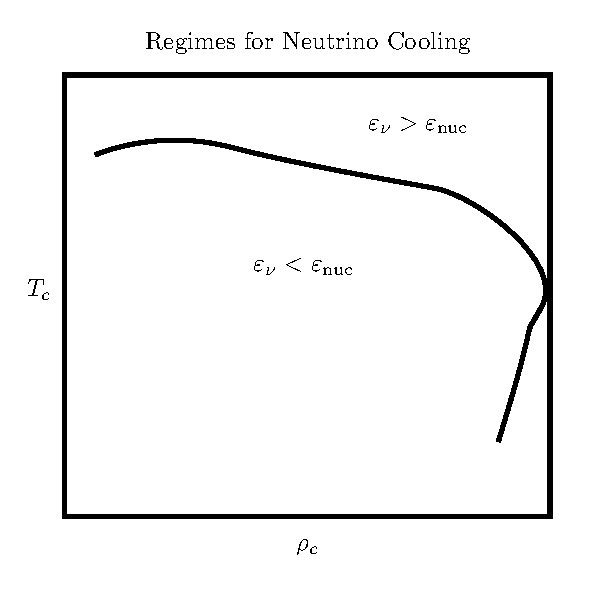
\includegraphics{neutrinoCool.pdf}
      \caption{Rough sketch of the limits where neutrino cooling becomes 
dominant.}
      \label{fig:cooling}
    \end{figure}
    \n If there is just carbon burning taking place, all of the carbon
    will eventually be burned, leaving oxygen unburned. Then oxygen,
    neon, and magnesium are the dominant elements. For stars between
    $6\,M_\odot$ and $8\,M_\odot$ where carbon is burned, electron
    degeneracy sets in, and they will die as white dwarfs.\\

    \n After carbon burning, we have ${}^{16}\mathrm{O}$,
    ${}^{20}\mathrm{Ne}$, and ${}^{23}\mathrm{Na}$ available. The
    ${}^{16}\mathrm{O}+{}^{16}\mathrm{O}$ reaction requires such a
    high temperature that prior to this, we have photodisintegration
    of neon:
    \begin{equation}
      \label{eq:361}
      \mathrm{\gamma+{}^{20}Ne\to \alpha+{}^{16}O}
    \end{equation}
    These alpha particle laying around get scooped up by neon (before
    Oxygen!):
    \begin{equation}
      \label{eq:362}
      \mathrm{\alpha+{}^{20}Ne\to\gamma+{}^{24}Mg}
    \end{equation}
    This leads to magnesium burning:
    \begin{equation}
      \label{eq:363}
      \mathrm{\alpha+{}^{24}Mg\to \gamma+{}^{28}Si}
    \end{equation}
    This process leaves us with oxygen, magnesium, and silicon.\\
    
%%%%%%%%%%%%%%%%%%%%%%%%%%
% Monday, March 12, 2012 %
%%%%%%%%%%%%%%%%%%%%%%%%%%
    \n \textit{Monday, March 12, 2012}\\
    
\section{Core Collapse and Stellar Death}
	\label{sec:core-collapse} 
	\subsection{The March to Collapse}
	\label{sec:march-to-collapse}
	Neutrino cooling ``resets'' the timescale for evolution, thereby 
accelerating the burning phases. Additionally, for nearly all these phases 
(carbon, neon, oxygen, etc.), the evolution times still remains longer than
	\begin{equation}
	\label{eq:364} t_{\mathrm{dyn}}\sim\frac{1}{\sqrt{G\rho}}=4\,\mathrm{s}
\,\left(\frac{10^{6}\,\mathrm{g\,cm^{-3}}}{\rho_{c}}\right)^{1/2}
	\end{equation}
	Meanwhile, the star is building up an onion skin shell struture of 
overlying layers of different elements. The burning up to ${}^{28}\mathrm
{Si}$ is still fusion driven. ${}^{28}\mathrm{Si}$ actually burns via 
\textbf{photodisintegration}:
	\begin{equation}
	\label{eq:365}{}^{28}\mathrm{Si}+{}^{28}\mathrm{Si}\to{}^{56}\mathrm
{Ni}
	\end{equation}
	This reaction has a prohibitive Coulomb barrier, so the following 
reaction is favored
	\begin{equation}
	\label{eq:366} \gamma+{}^{28}\mathrm{Si}\to\alpha+{}^{24}\mathrm{Mg}
	\end{equation}�
	Remember that at $T_{9}\sim 1$, we have $E_{\gamma}\sim 100\,\mathrm
{keV}$.\\
	
	\n The most stable element at fixed mass number $A$ are neutron rich 
($N>Z$). During silicon ``burning'', there is time for weak interactions, 
yielding more neutron-rich isotopes. Using beta captures, the pressure 
support is decreased.
	\subsection{Stellar Core Collapse}
	As the electrons in the core become relativistic, the mass of the core 
approaches the Chandrasekhar mass (appropriately corrected for temperature 
and the electrons per baryon, so lower than that for white dwarf). As the 
mass increases, the core compresses, making the electrons become more 
relativistic and also increasing the temperature. The electrons are 
captured by nuclei, and the photons photodisintegrate the nuclei, starting 
the undoing of all of the nucleosynthesis that has been going on in the 
star.\\

	\n Now we have to worry about energy \emph{sinks} in the star, since these reactions are endothermic. One such reaction is
	\begin{equation}
	\label{eq:367} \gamma+{}^{56}\mathrm{Fe}\to 13\alpha+4n
	\end{equation}
	Which requires an energy of 124 MeV. This energy comes from the ambient thermal energy, so the core is cooled, and thus contracts. The energy lost per unit mass is
	\begin{equation}
	\label{eq:368} \frac{124\,\mathrm{MeV}}{56m_{p}}=2\,\mathrm{MeV/baryon}
	\end{equation}
	The Contraction must get to
	\begin{equation}
	\frac{GM}{R}\approx 2\,\mathrm{MeV/baryon}
	\end{equation}
	Which gives for a star the mass of the sun being $R=1000\,\mathrm{km}$! Just considering the case where half of the ${}^{56}\mathrm{Fe}$ is destroyed, we get the data shown in Table \ref{tab:iron}.\\
	\begin{table}[h!]
	\centering
	\begin{tabular}{cc}
		$\rho_{9}$ & $T_{10}$\\
		\hline \hline
		0.1 & 0.78\\
		1 & 0.95\\
		10 & 1.2
	\end{tabular}
	\caption{Density and temperature of a degenerate core at half iron disintegration}
	\label{tab:iron}
	\end{table}
	
	\n Photodisintegration gets the radius down to less than 1000 km and the density up to $\rho_{10}\sim 1$. Since the electrons are relativistic, the Fermi energy is $E_{F}\sim m_{e}c^{2}$ (for the electrons). Now recall the Chandrasekhar mass,
	\begin{equation}
	\label{eq:369} M_{\mathrm{Ch}}=1.46\,M_{\odot}\left[\frac{Y_{e}}{1/2}\right]^{2}
	\end{equation}
	Where $Y_{e}$ is the number of electrons per baryon. For a pure C/O object, $Y_{e}=1/2$. For ${}^{56}\mathrm{Fe}$, though, $Y_{e}=0.46$, which introduces a correction for a \emph{cold} iron core, bringing the mass down to $1.26\,M_{\odot}$. As the Fermi energy increases, more electron captures occur, increasing the neutron-richness of the plasma.\\
	
	\n During the rest of the collapse, the nuclei are being broken up and more and more protons are converted to neutrons via electron capture, which also causes a flurry of neutrino emission. The collapse suddenly ``halts'' when a density is reached that implies the mean spacing is of order of the neutron radius, or 1 fm (fermi). Here we have the onset of an incompressible equation of state. That is, the pressure rises dramatically as the density approaches the nuclear density of about $\rho\approx \rho_{\mathrm{nuc}}\approx 10^{14}\,\mathrm{g\,cm^{-3}}$.\\
	
	\n At this point, the radius is about 15 km and the collapsed core ``halts'' at about 10 km. The gravitational potential energy is
	\begin{equation}
	E_{\mathrm{GR}}=\frac{GM^{2}}{R}=10^{53}\,\mathrm{ergs}
	\end{equation}
	So if a fraction of this energy is tapped, it would be enough to unbind the envelope (around $10^{51}\,\mathrm{ergs}$). As it turns out, the outgoing shock \emph{does} contain about $10^{52}\,\mathrm{ergs}$.
	
	\subsection{Neutron Star and Black Hole Formation}
	\label{sec:neutron-star} 
	The collapsed core is essentially a proto-neutron star with $E_{\mathrm{th}}=E_{\mathrm{GR}}=10^{53}\,\mathrm{ergs}$, which is strying to cool via thermal neutrino emission. The open question is how the outgoing shock succeeds in ``punching through'' the infalling matter.\\
	
	\n Cores in massive stars collapse when $M_{\mathrm{core}}>M_{\mathrm{crit}}$, where $M_{\mathrm{crit}}$ depends on the evolution of the star, details of the star's rotation, and the mass of the star. Collapses lead to a dense proto-neutron star with a radius of around 20 km and an outgoing shock.
	\end{document}

